\documentclass[palatino,nochap]{apuntes}

\usepackage{hyperref}

\usepackage{tikztools}
\usepackage{fastbuild}
\usepackage{tikz-3dplot}

\usepackage{tikz}
\usepackage{graphicx}
\usepackage{latexsym, amsfonts, amsmath, amssymb, amscd, epsfig,amsthm}
\usepackage{enumitem}
\usepackage{natbib}
\usepackage[nottoc]{tocbibind}
\usepackage{fancysprefs}

\setcounter{tocdepth}{3}

\lstset{
    language=R,
    basicstyle=\ttfamily
}


%%%%%%%%%%%%%%%  lstlisting style


\definecolor{codegreen}{rgb}{0,0.6,0}
\definecolor{codegray}{rgb}{0.5,0.5,0.5}
\definecolor{codepurple}{rgb}{0.58,0,0.82}
\definecolor{backcolour}{rgb}{0.95,0.95,0.92}

\lstdefinestyle{mystyle}{
    backgroundcolor=\color{backcolour},
    commentstyle=\color{codegreen},
    keywordstyle=\color{magenta},
    numberstyle=\tiny\color{codegray},
    stringstyle=\color{codepurple},
    basicstyle=\footnotesize,
    breakatwhitespace=false,
    breaklines=true,
    captionpos=b,
    keepspaces=true,
    numbers=left,
    numbersep=5pt,
    showspaces=false,
    showstringspaces=false,
    showtabs=false,
    tabsize=2
}



\usepackage{caption}



\bibliographystyle{plainnat}

\input xy
\xyoption{all} %%!!
\usetikzlibrary{calc, intersections}
\author{Víctor de Juan}
\date{2014/2015 2º cuatrimestre}

\renewcommand*{\arraystretch}{1.5}
\title{Estadística II}
% Lo comento porque creo que el incluir los PDFs abajo está reventando el precompile
%\precompileTikz

\begin{document}

\chapter{Distribución normal multivariante}

\section{Esperanza, varianza y covarianza de variables aleatorias}

Dada una variable aleatoria definimos:
\begin{itemize}
\item Esperanza: $\mu = \mathbb{E}(X) = \int_{-\infty}^{\infty}x\cdot f_P(x) dx$

Propiedades:
\begin{enumerate}
\item $\mathbb{E}(aX) = a\mathbb{E}(X)$
\item $\mathbb{E}(X+Y) = \mathbb{E}(X)+\mathbb{E}(Y)$
\item $\mathbb{E}(X+c) = \mathbb{E}(X)+c$ (La esperanza de una constante es la propia constante)
\end{enumerate}
\item Varianza: $Var(X) = \mathbb{E}((X-\mathbb{E}(X))^2) =\mathbb{E}((X-\mu)^2) = \mathbb{E}(X^2)-\mu^2$

Propiedades:
\begin{enumerate}
\item $Var(X+b)=Var(X)$
\item $Var(aX)=a^2Var(X)$
\item $Var(X)\geq 0$
\end{enumerate}
\item Covarianza (entre dos variables aleatorias $X_i$, $X_j$): $\sigma_{i,j} = Cov(X_i,X_j) = \mathbb{E}\left((X_i-\mathbb{E}(X_i))(X_j-\mathbb{E}(X_j))\right) = \mathbb{E}(X_i X_j)-\mathbb{E}(X_i)\mathbb{E}(X_j)$

Dos propiedades importantes de la covarianza son:

\begin{enumerate}
\item Cov(X,X)= Var(X)
\item $Cov(X,Y)=Cov(Y,X)$
\end{enumerate}

\end{itemize}

\section{Esperanza, varianza y covarianza de vectores aleatorios}

Un vector aleatorio es un vector de variables aleatorias.

Notación: como durante el curso vamos a trabajar con vectores aleatorios, vamos a generalizar los símbolos que iremos usando:
\begin{itemize}
\item $X = (X_1, X_2,...,X_p)'$ será un vector de p variables aleatorias. Las variables aleatorias serán $X_1, X_2,...,X_p$. La comilla simple $'$ indica que $X$ es un vector columna.
\item $\mu$ será la esperanza del vector aleatorio X: $\mathbb{E}(X)$. Las esperanzas de cada variable aleatoria serán $\mu_1, \mu_2,...,\mu_p$.
\item Si A es una matriz, A' es su traspuesta
\end{itemize}

Por tanto, dado un vector de p variables aleatorias (vector aleatorio p-dimensional), definimos:

\begin{itemize}
\item Esperanza. Será un vector columna con las esperanzas de cada variable aleatoria.
\[
\mathbb{E}(X) = \mu = (\mu_1, \mu_2,..., \mu_p)'
\]

Donde cada $\mu_i = \mathbb{E}(X_i)$.

Ejemplo p=3:
\[
\mathbb{E}(X)=
\mathbb{E}\left[
\left(
\begin{array}{c}
X_1\\
X_2\\
X_3
\end{array}
\right)
\right]=
\left(
\begin{array}{c}
\mathbb{E}(X_1)\\
\mathbb{E}(X_2)\\
\mathbb{E}(X_3)
\end{array}
\right)=
\left(
\begin{array}{c}
\mu_1\\
\mu_2\\
\mu_3
\end{array}
\right)=
\mu
\]

Propiedades:
\begin{enumerate}
\item $\mathbb{E}(X+c) = \mathbb{E}(X)+c$. Como en el caso de variables aleatorias.
\item $\mathbb{E}(AX) = A\mathbb{E}(X)$. Donde A es una matriz de dimensión $p$x$p$ siendo p la dimensión de X.

Lo vemos para p=3:

\[
\mathbb{E}(AX)=
\mathbb{E}\left[
\left(
\begin{array}{ccc}
a_{1,1}& a_{1,2}& a_{1,3}\\
a_{2,1}& a_{2,2}& a_{2,3}\\
a_{3,1}& a_{3,2}& a_{3,3}
\end{array}
\right)
\left(
\begin{array}{c}
X_1\\
X_2\\
X_3
\end{array}
\right) \right]=
\mathbb{E}\left[
\left(
\begin{array}{c}
a_{1,1}X_1 - a_{1,2}X_2 - a_{1,3}X_3\\
a_{2,1}X_1 - a_{2,2}X_2 - a_{2,3}X_3\\
a_{3,1}X_1 - a_{3,2}X_2 - a_{3,3}X_3
\end{array}
\right)
\right]=
\]

\[
=\left(
\begin{array}{c}
a_{1,1}\mathbb{E}(X_1) - a_{1,2}\mathbb{E}(X_2) - a_{1,3}\mathbb{E}(X_3)\\
a_{2,1}\mathbb{E}(X_1) - a_{2,2}\mathbb{E}(X_2) - a_{2,3}\mathbb{E}(X_3)\\
a_{3,1}\mathbb{E}(X_1) - a_{3,2}\mathbb{E}(X_2) - a_{3,3}\mathbb{E}(X_3)
\end{array}
\right)=
\left(
\begin{array}{ccc}
a_{1,1}& a_{1,2}& a_{1,3}\\
a_{2,1}& a_{2,2}& a_{2,3}\\
a_{3,1}& a_{3,2}& a_{3,3}
\end{array}
\right)
\left(
\begin{array}{c}
\mathbb{E}(X_1)\\
\mathbb{E}(X_2)\\
\mathbb{E}(X_3)
\end{array}
\right)=
\]
\[
=A\mathbb{E}(X)
\]

\end{enumerate}

\item Varianza. La varianza va a ser una matriz, donde cada elemento va a ser la covarianza entre dos de las p variables aleatorias que conforman el vector. Será por tanto una matriz simétrica (ya que $\sigma_{i,j}=Cov(X_i,X_j)=Cov(X_j,X_i)=\sigma_{j,i}$). La matriz resultante será la llamada matriz de covarianzas $\Sigma$.
\[
Var(X)=\mathbb{E}\left((X-\mu)(X-\mu)'\right) = \mathbb{E}(XX')-\mu \mu'=\Sigma
\]

\begin{proof}
\[
Var(X)=\mathbb{E}\left((X-\mu)(X-\mu)'\right) = \mathbb{E}(XX'- \mu X' - X \mu'+\mu \mu')=
\]
\[
\mathbb{E}(XX')-\mathbb{E}(\mu X')-\mathbb{E}(X\mu')+\mathbb{E}(\mu \mu')= \mathbb{E}(XX')-\mu \mathbb{E}(X')-\mu' \mathbb{E}(X)+\mu\mu'=
\]
\[
 \mathbb{E}(XX')-\mu \mu'-\mu' \mu+\mu \mu' = \mathbb{E}(XX')-\mu \mu'=\Sigma
\]
\end{proof}

Ejemplo p=3:

\[
Var(X)=
\mathbb{E}\left[
\left(
\begin{array}{c}
X_1-\mu_1\\
X_2-\mu_2\\
X_3-\mu_3
\end{array}
\right)
(X_1-\mu_1, X_2-\mu_2, X_3-\mu_3)\right]=
\left(
\begin{array}{ccc}
\sigma_{1,1}& \sigma_{1,2}& \sigma_{1,3} \\
\sigma_{2,1}& \sigma_{2,2}& \sigma_{2,3} \\
\sigma_{3,1}& \sigma_{3,2}& \sigma_{3,3}
\end{array}
\right)=
\]

\[
=\left(
\begin{array}{ccc}
Var(X_1)& \sigma_{1,2}& \sigma_{1,3} \\
\sigma_{2,1}& Var(X_2)& \sigma_{2,3} \\
\sigma_{3,1}& \sigma_{3,2}& Var(X_3)
\end{array}
\right) = \Sigma
\]

Donde se cumple que $\sigma_{1,2}=\sigma_{2,1}$, $\sigma_{1,3}=\sigma_{3,1}$ y $\sigma_{3,2}=\sigma_{2,3}$. Y por tanto $\Sigma$ es simétrica.
\end{itemize}




\textcolor{red}{Mirar si tiene importancia lo de $\Sigma$ semidefinida positiva y tal}

\section{Función característica}
La función característica de un vector aleatorio X es:
\[
\phi_X(t)=\mathbb{E}(e^{it'X})
\]

Siendo X y t p-dimensionales.

Se llama función característica porque es única para cada distribución de X. Es decir:
\begin{prop} Sean X e Y dos vectores aleatorios:
\[
\phi_X(t)=\phi_Y(t) \Leftrightarrow X \stackrel{d}{=} Y
\]
\end{prop}

\begin{prop} Mecanismo de Cramer-Wold: Dados dos vectores aleatorios X e Y:
\textcolor{red}{preguntar que es a'X (dos vectores columna multiplicados?)}
\[
a'X \stackrel{d}{=} a'Y \text{ } \forall a \in \mathbb{R}^p \Leftrightarrow X \stackrel{D}{=} Y
\] 
\begin{proof}
\begin{itemize}
\item $\Leftarrow)$ Trivial
\item $\Rightarrow)$ Aplicamos la función característica y tenemos que:
$$\phi_{a'X}(t) \phi_{a'Y}(t) \text{ } \forall t \in \mathbb{R}$$

Por tanto, también es cierto para t=1:
$$\phi_{a'X}(1) = \phi_{a'Y}(1) \Rightarrow \mathbb{E}(e^{ia'X})=\mathbb{E}(e^{ia'Y}) \Rightarrow \phi_{X}(a)=\phi_{Y}(a)$$
\end{itemize}
\end{proof}
\end{prop}

Esta función caracteriza la distribución de X:




\section{Matriz de covarianzas}
Como ya dijimos anteriormente la matriz de covarianzas $\Sigma$ define la varianza de un vector aleatorio y es simétrica. Por tanto podemos expresar $\Sigma$ de la siguiente forma:
\[
\Sigma = CDC^{-1}
\]

Siendo D una matriz diagonal.

$C^{-1}=C'$ ya que las columnas de C son vectores ortonormales.
Por tanto:
\[
\Sigma = CDC'  \text{ y } \Sigma^{-1} = CD^{-1}C'
\]

Ejemplo p=2:
\[
\mu=\left(
\begin{array}{c}
0\\
0
\end{array}
\right)
\text{ , }
\Sigma=\left(
\begin{array}{cc}
\lambda_1& 0 \\
0 & \lambda_2
\end{array}
\right)
\]
Tenemos:
\[
(X_1, X_2)
\left(
\begin{array}{cc}
\lambda_1& 0 \\
0 & \lambda_2
\end{array}
\right)
\left(
\begin{array}{c}
X_1\\
X_2
\end{array}
\right) = cte
\Rightarrow
\frac{X_1^2}{\lambda_1}+\frac{X_2^2}{\lambda_2}=cte
\]
Luego:
\[
(X-\mu)'\Sigma(X-\mu) = cte \Rightarrow (X-\mu)'CD^{-1}C'(X-\mu) = cte \Rightarrow (\tilde{X}-\tilde{\mu})'CD^{-1}C'(\tilde{X}-\tilde{\mu}) = cte
\]

\begin{defn}[Correlación]
La correlación entre dos vectores aleatorios $X_1$ y $X_2$ se define como:
\[
cor(X_1,X_2)=\frac{cov(X_1,X_2)}{\sqrt{Var(X_1)Var(X_2)}}
\]

Es por tanto una matriz, en su diagonal principal esta formada por 1's. \textcolor{red}{Explicar algo más del significado geométrico de la correlación}


\end{defn}

\section{Estandarización multivariante}
\begin{defn}
Sea X una variable aleatoria. X es normal si tiene densidad dada por:
\[
f(x) = \frac{1}{\sigma\sqrt{2 \pi}}e^{-\frac{(x-\mu)^2}{2\sigma^2}}
\]

Además, si cogemos $Y=\frac{X-\mu}{\sigma}$ entonces $Y\equiv N(0,1)$
\end{defn}

\begin{defn}
Sea un vector aleatorio X, es normal p-dimensional con vector de medias $\mu$ y matriz de covarianzas $\Sigma$ (notación: $X\equiv N_p(\mu, \Sigma)$) si tiene densidad dada por:

\[
f(x)=\abs{\Sigma}^{-1/2}(2\pi)^{-p/2} e^{\left( -\frac{1}{2}(x-\mu)'\Sigma^{-1}(x-\mu) \right)}
\]
\end{defn}

\begin{prop} Si $X \equiv N_p(\mu, \Sigma)$ y definimos $Y = \Sigma^{-1/2}(X-\mu)$, entonces $Y_1,...,Y_p$ son i.i.d. N(0,1).\end{prop}

\begin{proof}
Sabemos por definición que:
\[
f_X(x)=\abs{\Sigma}^{-1/2}(2\pi)^{-p/2} \exp \left\{ -\frac{1}{2}(x-\mu)'\Sigma^{-1}(x-\mu) \right\}
\]

Vamos a aplicar un cambio de variable en la fórmula de la densidad:

Despejando de $Y = h(X)= \Sigma^{-1/2}(X-\mu)$, obtenemos que $\Sigma^{1/2}Y+\mu=h^{-1}(Y)=X$.

Y ahora cogemos el Jacobiano de $h^{-1}(Y)=X$ que será $\Sigma^{1/2}$ ($\mu$ es una constante e Y es la variable).

\textcolor{red}{Esto de coger el jacobiano a qué se debe? A que luego la función de densidad se integra?}


Por tanto nos quedaría:
\[
f(x) = \abs{\Sigma}^{-1/2}(2\pi)^{-p/2} \exp \left\{ -\frac{1}{2}(x-\mu)'\Sigma^{-1}(x-\mu) \right\} = f(h^{-1}(y))\cdot\abs{Jh(x)} =
\]
\[ 
\abs{\Sigma}^{-1/2}(2 \pi)^{-p/2} \exp\left\{-\frac{1}{2}(\Sigma^{1/2}y+\mu-\mu)'\Sigma^{-1}(\Sigma^{1/2}y+\mu-\mu)  \right\} \abs{\Sigma^{1/2}}  =
\]
\[
= \abs{\Sigma}^{-1/2}(2 \pi)^{-p/2} \exp\left\{-\frac{1}{2}y'\Sigma'^{1/2}\Sigma^{-1}\Sigma^{1/2}y)  \right\} \abs{\Sigma}^{1/2} =
\]

Por ser $\Sigma$ simétrica tenemos que: $\Sigma = \Sigma'$
\[
= \abs{\Sigma}^{-1/2}(2 \pi)^{-p/2} \exp\left\{-\frac{1}{2}y'\Sigma^{1/2}\Sigma^{-1}\Sigma^{1/2}y)  \right\} \abs{\Sigma}^{1/2} =
\]
\[
= (2 \pi)^{-p/2} \exp\left\{-\frac{1}{2}(y'y) \right\} = \prod_{i=1}^{p} \frac{1}{\sqrt{2\pi}} e^{-\frac{(y_i)^2}{2}} =  \prod_{i=1}^{p} \frac{1}{\sqrt{2\pi}} e^{-\frac{(x_i-\mu)^2}{2\sigma^2}} =\prod_{i=1}^{p} f_{X_{i}}(x)
\]

\textcolor{red}{Multiplicamos un vector columna por un vector fila, sería al reves no?}

Hemos usado un teorema que dice que n variables aleatorias $X_1,...,X_n$ son independientes si y solo si el $f(x_1,...,x_n)=\prod_{i=1}^{n}f(x_i)$ siendo f la función de densidad.

\end{proof}

\textcolor{blue}{Comprobar esto:}
\begin{obs}
Si $X \equiv N_p(\mu, \Sigma)$ y definimos $Y = \Sigma^{-1/2}(X-\mu)$, entonces $Y\equiv N_p(0_p, I_p)$. Siendo $0_p$ un vector de 0's de dimensión p, e I la matriz identidad de rango p:
\end{obs}
\[
\mathbb{E}(Y)=\mathbb{E}\left( \Sigma^{-1/2}(X-\mu) \right) = \Sigma^{-1/2} \mathbb{E}\left( (X-\mu) \right) = \Sigma^{-1/2}(\mu -\mu)=0
\]

\[
Var(Y)=Var\left(\Sigma^{-1/2}(X-\mu) \right)=
\]
\[
=\mathbb{E}\left( \left( \Sigma^{-1/2}X-\Sigma^{-1/2}\mu-\Sigma^{-1/2}\mu+\Sigma^{-1/2}\mu \right) \left( \Sigma^{-1/2}X-\Sigma^{-1/2}\mu-\Sigma^{-1/2}\mu+\Sigma^{-1/2}\mu \right)' \right)=
\]
Usamos que $\Sigma$ es simétrica:
\[
=\mathbb{E}\left( \left( \Sigma^{-1/2}(X-\mu) \right) \left( \Sigma^{-1/2}(X-\mu) \right)' \right) = \mathbb{E}\left( \Sigma^{-1/2}(X-\mu)(X-\mu)'\Sigma^{-1/2}  \right) = \Sigma^{-1/2}\Sigma\Sigma^{-1/2} = I
\]


\textbf{Estandarización paso por paso: }Vamos a ver qué es lo que hacemos con la estandarización paso por paso. Sea X el vector aleatorio:
\begin{enumerate}
\item $Y=(X-\mu)$. Aquí lo que hacemos es simplemente una traslación del vector X. 
\item $Y=C'(X-\mu)$. Aquí giramos los datos. C' es una matriz de giro ya que su determinante es 1 (de hecho es ortonormal). Esta rotación elimina la correlación \textcolor{red}{¿Por qué?}. Calculamos la varianza:
\[
Var\left( C'(X-\mu) \right) = \mathbb{E}\left( \left( C'X-C'\mu-C'\mu+C'\mu \right) \left( C'X-C'\mu-C'\mu+C'\mu \right)' \right)
\]
\[
\mathbb{E}\left( \left( C'(X-\mu) \right) \left( C'(X-\mu) \right)' \right) = \mathbb{E}\left( C'(X-\mu)(X-\mu)'C  \right) = C'\Sigma C=C'CDCC'=D
\]
\item $Y=D^{-1/2}C'(X-\mu)$. Con esto hacemos un cambio de escala para que las varianzas sean 1. Calculamos la varianza. Usamos que $Var(AX)=AVar(X)A'$ y que $D=D'$:
\[
Var\left( D^{-1/2}C'(X-\mu) \right) = D^{-1/2}DD^{-1/2} = I
\]
\item $Y=CD^{-1/2}C'(X-\mu)$. Deshacemos el giro de antes. Calculamos la varianza:
\[
Var\left( CD^{-1/2}C'(X-\mu) \right)=CIC' = I
\]
\end{enumerate}
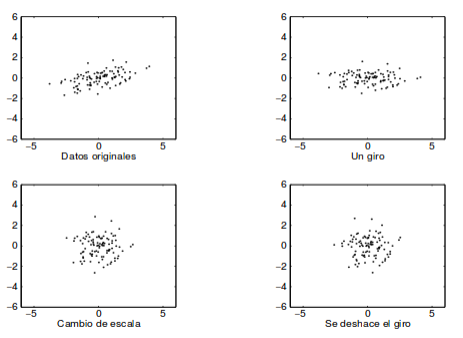
\includegraphics[scale=0.75]{img/estandarizacionMultivariante.png}

\textbf{Consecuencias de la estandarización:}
\begin{enumerate}
\item Si $X\equiv N_p(\mu, \Sigma)$, entonces $\mathbb{E}(X)=\mu$ y $Var(X)=\Sigma$.

Esto es cierto ya que tal y como hemos visto antes $X=\Sigma{1/2}Y+\mu$ y entonces  (Usando que $C'=C$)$\mathbb{E}(X)=0+\mu$ y $Var(X)=Var(\Sigma{1/2}Y+\mu)=Var(\Sigma{1/2}Y)=\Sigma^{1/2}Var(Y)\Sigma'^{1/2}=CD^{1/2}C'IC'D^{1/2}C=\Sigma$

\item Si $X\equiv N_p(\mu, \Sigma)$, entonces $\phi_X(t)=exp\left\{ it'\mu-\frac{1}{2}t'\Sigma t \right\}$:
%\[
%\phi_X(t)=\mathbb{E}\left( exp\left\{ it'(\Sigma^{1/2}Y+\mu) \right\} \right) = exp \left\{ it'\mu  \right\} \mathbb{E}\left( exp\left\{ it'\Sigma^{1/2}Y \right\} \right)
%\]
\item La distribución de $(X-\mu)'\Sigma(X-\mu)$ es $\chi^2_p$:

Siendo $X\equiv N_p(\mu,\Sigma)$ con $X=\Sigma^{-1/2}Y+\mu$. Entonces (sabiendo que $\Sigma$ es simétrica):
\[
(X-\mu)'\Sigma^{-1}(X-\mu)=Y'\Sigma^{1/2}\Sigma^{-1}\Sigma^{1/2}Y=Y'Y=\sum_{i=1}^{p} Y_i^2
\]
\textcolor{red}{Otra vez líos con vector columna o fila}
Usando que $Y_i\equiv N(0,1)$, entonces:
\[
\sum_{i=1}^{p} Y_i^2 = \chi^2_p \text{ chi-cuadrado con p grados de libertad}
\]

\end{enumerate}

\section{Transformaciones afines de vectores normales}
\begin{prop}
Si $X \equiv N_p(\mu, \Sigma)$, A es matriz qxp y $b\in \mathbb{R}^q$, entonces $AX+b \equiv N_q(A\mu +b, A\Sigma A')$
\end{prop}
\begin{proof}
\[
\phi_[AX+b](t)=\mathbb{E}\left( exp\left\{ it'(AX+b) \right\} \right) = e^{it'b}\mathbb{E}\left( e^{it'AX} \right) = e^{it'b} exp\left\{ it'A\mu-\frac{1}{2}t'A\Sigma A't \right\}
\]
\textcolor{blue}{sin terminar...}
\end{proof}

Una consecuencia de esta proposición es lo siguiente: Si X sigue una distribución normal p-dimensional, y se expresa como $X=(X_1|X_2)$, con $X_1\in \mathbb{R}^q$ y $X_2\in \mathbb{R}^{p-q}$, y consideramos las particiones correspondientes de $\mu$ y $\Sigma$:
\[
\mu=(\mu_1 | \mu_2) \text{ , } \Sigma=
\left(
\begin{array}{c|c}
\Sigma_{11}& \Sigma_{12} \\
\hline
\Sigma_{21}& \Sigma_{22} 
\end{array}
\right)
\]
entonces $X_1\equiv N_q(\mu_1, \Sigma_{11})$

\begin{example}
Sea un vector de variables aleatorias $Y=(Y_1, Y_2,Y_3, Y_4, Y_5)$ tal que $Y\equiv N_5(\mu, \Sigma)$ (Y es normal 5-dimensional) con vector de medias $\mu=(\mu_1, \mu_2, \mu_3, \mu_4, \mu_5)$ y sea $X_1=(Y_1,Y_2,Y_3)$ y $X_2=(Y_4,Y_5)$. 

\[
\mu=
\left(
\begin{array}{c}
\mu_{X_1}\\
\hline
\mu_{X_2}
\end{array}
\right)=
\left(
\begin{array}{c}
\mu_{Y_1}\\
\mu_{Y_2}\\
\mu_{Y_3}\\
\hline
\mu_{Y_4}\\
\mu_{Y_5}
\end{array}
\right)
\]
\[
\Sigma_Y=
\left(
\begin{array}{ccc|cc}
\Sigma_{11}& \Sigma_{12} & \Sigma_{13} & \Sigma_{14} & \Sigma_{15}\\
\Sigma_{21}& \Sigma_{22} & \Sigma_{23} & \Sigma_{24} & \Sigma_{25}\\
\Sigma_{31}& \Sigma_{32} & \Sigma_{33} & \Sigma_{34} & \Sigma_{35}\\
\hline
\Sigma_{41}& \Sigma_{42} & \Sigma_{43} & \Sigma_{44} & \Sigma_{45}\\
\Sigma_{51}& \Sigma_{52} & \Sigma_{53} & \Sigma_{54} & \Sigma_{55}
\end{array}
\right) \text{ , }
\Sigma_X=
\left(
\begin{array}{c|c}
\Sigma_{11}& \Sigma_{12} \\
\hline
\Sigma_{21}& \Sigma_{22} 
\end{array}
\right)
\]

Entonces $X_1\equiv N_3(\mu_{X_1}, \Sigma_{11})$ para la matriz $\Sigma_X$.
\end{example}

\begin{prop}
\textcolor{red}{Si $X=(X_1,X_2)$ es normal n-dimensional siendo n la suma de la dimension de $X_1+X_2$, entonces :}Dado $X_1$ y $X_2$ vectores aleatorios, son independientes si y solo si $\Sigma_{12}=\Sigma_{21}=0$
\end{prop}

\begin{obs}
\begin{itemize}
\item Si dos variables aleatorias tienen distribución normal y además $Cov(X,Y)=0$, esto no implica que X e Y sean independientes. Esto sería cierto si el vector (X,Y) fuera normal bidimensional.
\item Si dos variables aleatorias X e Y tienen distribución normal y $a,b \in \mathbb{R}$, la combinación linear de $aX+bY$ no tiene necesariamente distribución normal. Esto sería cierto si el vector (X,Y) fuera normal bidimensional.
\item Aunque todas las marginales de un vector aleatorio p-dimensional X tengan distribución normal, esto no implica que X tenga distribución normal p-dimensional. Esto sería cierto si todas ellas fueran independientes entre si.
\end{itemize}
\end{obs}

\section{Ejercicio 1}
Definimos el siguiente vector aleatorio: $X = (X_1,X_2,X_3)' \equiv N_3(\mu, \Sigma)$ con:

\[
\mu=
\left(
\begin{array}{c}
0\\
0\\
0
\end{array}
\right) \text{,       }
\Sigma=
\left(
\begin{array}{ccc}
7/2& 1/2& -1 \\
1/2& 1/2& 0 \\
-1& 0& 1/2
\end{array}
\right)
\]

\ppart Calcula las distribuciones marginales $X_i \equiv N(\mathbb{E}(X_i), Var(X_i))$:

$X_1\equiv N(0, 7/2)$

$X_2\equiv N(0, 1/2)$

$X_3\equiv N(0, 1/2)$

Para calcular estos valores solo hace falta mirar los datos que nos da el problema, el vector de medias $\mu$ y la matriz de covarianzas $\Sigma$:

\[
\Sigma=\left(
\begin{array}{ccc}
Var(X_1)& \sigma_{1,2}& \sigma_{1,3} \\
\sigma_{2,1}& Var(X_2)& \sigma_{2,3} \\
\sigma_{3,1}& \sigma_{3,2}& Var(X_3)
\end{array}
\right)
\]

\[
\mu=
\left(
\begin{array}{c}
\mathbb{E}(X_1)\\
\mathbb{E}(X_2)\\
\mathbb{E}(X_3)
\end{array}
\right)=
\left(
\begin{array}{c}
\mu_1\\
\mu_2\\
\mu_3
\end{array}
\right)
\]

\ppart Calcula la distribución del vector $(X_1,X_2)'$:

Este vector sigue una distribución normal que puede obtener de las matriz $\Sigma$ y el vector de medias $\mu$:
\[
\left(
\begin{array}{c}
X_1\\
X_2
\end{array}
\right)
\equiv N_2\left[
\left(
\begin{array}{c}
0\\
0
\end{array}
\right)
\text{, }
\left(
\begin{array}{cc}
7/2& 1/2 \\
1/2 & 1/2
\end{array}
\right)
\right]
\]

\ppart ¿Son $X_2$ y $X_3$ independientes?

Sí son independientes ya que la covarianza entre ambas variables es 0. La covarianza entre $X_2$ y $X_3$ es el elemento de la fila 3 y la columna 2 de la matriz de covarianzas $\Sigma$, (que al ser $\Sigma$ simétrica coincide con el elemento de la fila 2 y la columna 3).

\ppart ¿Es $X_3$ independiente del vector $(X_1, X_2)'$?
No, no lo es, tenemos que ver que ciertos elementos de la matriz de covarianzas son 0:
\[
\Sigma=
\left(
\begin{array}{cc|c}
7/2& 1/2& -1 \\
1/2& 1/2& 0 \\
\hline
-1& 0& 1/2
\end{array}
\right)
\]

Y vemos que hay un '-1' y un '0', si fueran los dos elementos 0, si serían independientes, pero al haber un elemento distinto de 0, no lo son.


\ppart Calcula la  distribución de la variable aleatoria $(2X_1-X_2+3X_3)$. Utilizando la proposición anterior:

Si $X \equiv N_p(\mu, \Sigma)$, A es matriz qxp y $b\in \mathbb{R}^q$, entonces $AX+b \equiv N_q(A\mu +b, A\Sigma A')$ 

Procedemos de la siguiente manera: $X\equiv N_3(\mu, \Sigma)$, $A=(2,-1,3)$ tiene dimensión 1x3 y b=0. Por tanto:
\[
\mu=AX+b = (2,-1,3)\cdot
\left(
\begin{array}{c}
0 \\
0 \\
0
\end{array}
\right) = 0 
\]

\[
\Sigma = A\Sigma A'=(2,-1,3)
\left(
\begin{array}{ccc}
7/2& 1/2& -1 \\
1/2& 1/2& 0 \\
-1& 0& 1/2
\end{array}
\right) \left(
\begin{array}{c}
2 \\
-1 \\
3
\end{array}
\right)=5
\]

Por tanto, $(2X_1-X_2+3X_3)\equiv N(0,5)$



\section{Distribuciones condicionadas}

\begin{prop}

Sea $X=(X_1|X_2)$ con $X_1∈ℝ^p$ y $X_2∈ℝ^{p-q}$. Consideramos las particiones correspondientes de $µ$ y de $\Sigma$ y suponemos que $\Sigma_{11}^{-1}$ existe. Entonces:
\[
X_2|X_1 \equiv N_{p-q}(\mu_{2.1},\Sigma_{2.1})
\]
donde:
\[
\mu_{2.1}=\mu_2 +\Sigma_{21}\Sigma_{11}^{-1}(X_1-\mu_1)
\]
\[
\Sigma_{2.1}=\Sigma{22}-\Sigma_{21}\Sigma_{11}^{-1}\Sigma_{12}
\]

\begin{itemize}
\item $\mu_{2.1}=\mathbb{E}(X_2|X_1)$ es una función lineal (afín) de $X_1$
\item $\Sigma_{2.1}$ no depende de $X_1$ (homocedasticidad)
\end{itemize}

\end{prop}

\begin{example}

Sea \[\left(
\begin{array}{c}
X \\
Y
\end{array}
\right) \equiv N_2 \left( \left(
\begin{array}{c}
0 \\
0
\end{array}
\right), \begin{pmatrix}10&3\\3&1\end{pmatrix} \right)\]

A)Distribución $Y|X$:
Y hace de $X_2$ en la fórmula vista anteriormente (es el segundo elemento del vector), y X de $X_1$.

\[
\mu_{2.1}=E(Y|X)=\mu_2+\Sigma_{21}\Sigma_{11}^{-1}(X-\mu_1)=0+3\cdot \frac{1}{10}\cdot X = \frac{3}{10}X
\]
\[
\Sigma_{2.1}=V(Y|X) = \Sigma_{22}-\Sigma_{21}\Sigma_{11}^{-1}\Sigma_{12} = 1-3\cdot\frac{1}{10}\cdot3 = \frac{1}{10}
\]

B)Distribución $X|Y$:
Al hacer la distribución de $X_1|X_2$ cambiamos el orden de los índices en las fórmulas:

\[
\mu_{1.2}=E(X|Y)=\mu_1+\Sigma_{12}\Sigma_{22}^{-1}(Y-\mu_2)=0+3\cdot \frac{1}{1}\cdot Y = 3Y
\]
\[
\Sigma_{1.2}=V(X|Y) = \Sigma_{11}-\Sigma_{12}\Sigma_{22}^{-1}\Sigma_{21} = 10-3\cdot\frac{1}{1}\cdot3 = 1
\]

\end{example}


\begin{example}

Sea \[\left(
\begin{array}{c}
X \\
Y
\end{array}
\right) \equiv N_2 \left( \left(
\begin{array}{c}
1 \\
1
\end{array}
\right), \begin{pmatrix}3&1\\1&2\end{pmatrix} \right)\]

Sea $Z_1 = X+Y$ y $Z_2 = X-Y$. Calcula la  distribución condicionada de $Z_1$ a $Z_2=1$

Primero vamos a calcular el vector aleatorio $(Z_1,Z_2)$, por la proposición vista anteriormente tenemos que: $Z_1 \equiv N(A\mu+b,A\Sigma A')$ con:
\[
A=
\left(
\begin{array}{cc}
1 & 1 \\
1 & -1
\end{array}
\right)
\]

Nos queda:
\[
A\mu =
\left(
\begin{array}{cc}
1 & 1 \\
1 & -1
\end{array}
\right)
\left(
\begin{array}{c}
1 \\
1
\end{array}
\right)
=
\left(
\begin{array}{c}
2 \\
0
\end{array}
\right)
\]

Y por otro lado:
\[
A\Sigma A' =
\left(
\begin{array}{cc}
1 & 1 \\
1 & -1
\end{array}
\right)
\left(
\begin{array}{cc}
3& 1 \\
1& 2 
\end{array}
\right)
\left(
\begin{array}{cc}
1 & 1 \\
1 & -1
\end{array}
\right) =
\left(
\begin{array}{cc}
7 & 1 \\
1 & 3
\end{array}
\right)
\]

Por tanto nos queda:
\[\left(
\begin{array}{c}
Z_1 \\
Z_2
\end{array}
\right) \equiv N_2 \left( \left(
\begin{array}{c}
2 \\
0
\end{array}
\right), \begin{pmatrix}7&1\\1&3\end{pmatrix} \right)\]

Ahora vamos a calcular la distribución de $Z_1|Z_2$, otra vez tenemos los subíndices cambiados con respecto a la fórmula general, por tanto:
\[
\mu_{1.2}=E(Z_1|Z_2)=2+\frac{1}{3}Z_2 \stackrel{Z_2=1}{\Rightarrow} \frac{7}{3}
\]
\[
\Sigma_{1.2}=V(Z_1|Z_2) = 7-\frac{1}{3} = \frac{20}{3}
\]
Por tanto:
\[
\left(
Z_1|Z_2 \\
\right) \equiv N_2 \left( 
\frac{7}{3}
,  \frac{20}{3} \right)\]

\end{example}

\chapter{Contrastes no paramétricos}
Hipótesis no paramétrica: hipótesis que no se formula en términos de un número finito de parámetros.

\begin{enumerate}
\item \textbf{Bondad de ajuste}: A partir de una muestra $X_1,...,X_n \stackrel{iid}{\sim} F$ de observaciones ({\textcolor{red}{Parra: son muestras o variables aleatorias o es simple notación?}}{\textcolor{blue}{Jorge: son muestras que provienen de v.a. $X_i$ con distribución F}}) ($\stackrel{iid}{\sim}$ significa que son muestras aleatorias independientes idénticamente distribuidas que siguen una distribución F en este caso), contrastar:
\begin{itemize}
\item $H_0: F=F_0$ donde $F_0$ es una distribución prefijada.
\item $H_0: F \in \{F_{\theta} : \theta\in H\}$ H es el espacio paramétrico.
\end{itemize}
\item \textbf{ Homogeneidad}: Dados $X_1,...,X_n \stackrel{iid}{\sim} F$ y $Y_1,...,Y_n \stackrel{iid}{\sim} G$ de observaciones. Contrastar $H_0: F=G$.

(Por ejemplo para ver si el salario de los hombres $F$ tiene la misma distribución que el de las mujeres $G$).

\item \textbf{Hipótesis de independencia}: Dada $(X_1,Y_1),...,(X_n,Y_n) \stackrel{iid}{\sim} F$ de observaciones. Contrastar $H_0: X$ e $Y$ son independientes.

(Por ejemplo para $X$ salario e $Y$ sexo, querríamos ver si el salario es independiente del sexo).
\end{enumerate}

Antes de explicar los contrastes en detalle, vamos a definir y tratar de entender bien algunos conceptos. (quien ya lo entienda que pase de este apartado, que el profesor no lo ha explicado):

\begin{defn}{\textbf{$H_0$ = Hipótesis nula. }}
Más que una definición, es una interpretación: La hipótesis nula es lo que queremos rechazar cuando hacemos el contraste de hipótesis.

\begin{expla}
Es decir, nosotros lo que hacemos es obtener una muestra empírica de unos datos, y lo que vamos a hacer es mirar si podemos decir que NO siguen una distribución en concreto, o por el contrario, no podemos decir nada. Por tanto, el objetivo del contraste es ver si podemos rechazar que los datos siguen esa distribución definida por la hipótesis nula. Pero cuidado, el que no la rechacemos no significa que los datos sigan la distribución, sino que no tenemos suficiente evidencia estadística para afirmar que NO la siguen....
\end{expla}
\end{defn}


\begin{defn}{\textbf{$\alpha$ = nivel de significación. }}
Es la probabilidad máxima que queremos tener de equivocarnos si rechazamos la hipótesis nula. No depende de nada, lo asignamos nosotros en cada problema que queramos resolver.

\begin{expla}
Es decir, si hacemos un contraste de hipótesis con un nivel de significación $\alpha =0.05$, quiere decir, que si finalmente rechazamos la hipótesis nula, asumimos que lo estamos haciendo con un máximo de un $5\%$ de probabilidades de equivocarnos.
\end{expla}
\end{defn}

\begin{defn}{\textbf{p-valor. }}
valor de $\alpha$ mínimo con el que se empieza a rechazar la hipótesis nula. Depende de los datos de partida y de la hiṕotesis nula.
\begin{expla}
Interpretación del p-valor: El p-valor es un número entre 0 y 1, y representa la probabilidad que tenemos de equivocarnos si rechazamos la hipótesis nula. Dicho de otra forma,  el p-valor nos muestra la probabilidad de haber obtenido el resultado que hemos obtenido si suponemos que la hipótesis nula es cierta.

Razonémoslo con un ejemplo:
Supongamos que el p-valor sale 0.40. Esto quiere decir que si rechazamos la hipótesis nula, tenemos un $40\%$ de posibilidades de equivocarnos, por tanto, lo mejor es no rechazarla. Esto cuadra con la teoría, ya que si el p-valor es 0.40 (bastante alto), su valor estadístico asociado (T), es muy pequeño, y por tanto la región de rechazo ($R=\{T>c\}$) es bastante pequeña.

Según la otra interpretación tenemos que el resultado que hemos obtenido tendría un $40\%$ de posibilidades de obtenerse si consideramos que las variables aleatorias siguen la distribución que indica la hipótesis nula (en lugar de la que nos sale empíricamente). Esto también es razonable, ya que un $40\%$ es una probabilidad bastante alta como para rechazarla, por tanto, lo que hacemos es no rechazar la hipótesis nula.

Sin embargo, si nos sale un p-valor igual a 0.01, quiere decir que si rechazamos la hipótesis nula tenemos un $1\%$ de posibilidades de equivocarnos, que es bastante poco, por tanto, tenderemos a rechazarla.
\end{expla}
\end{defn}

Ahora vamos a ver la relación entre el p-valor y el nivel de significación:
\begin{expla}
Supongamos que queremos hacer el contraste de hipótesis con $\alpha=0.05$ y con una hipótesis nula $H_0$ cualquiera. Estudiamos los datos, y obtenemos un p-valor de 0.40. Por tanto, esto significa que si rechazamos la hipótesis nula tendríamos un $40\%$ de posibilidades de equivocarnos. Como nuestro $\alpha=0.05$ significa que solo estamos dispuestos a rechazar la hipótesis nula si tuviéramos un $5\%$ de probabilidades de equivocarnos, pero hemos visto que tenemos un $40\%$, por tanto, no rechazamos.

Supongamos ahora que queremos hacer el contraste de hipótesis con $\alpha=0.05$ pero obtenemos un p-valor de $0.02$. Por tanto, esto significa que si rechazamos la hipótesis nula tendríamos un $2\%$ de equivocarnos. Como hemos decidido que estamos dispuestos a rechazar la hipótesis nula con hasta un $5\%$ de probabilidades de equivocarnos, rechazamos. Si por el contrario imponemos $\alpha=0.01$, no rechazaríamos ya que sólo estaríamos dispuestos a equivocarnos como máximo un $1\%$ de las veces, y el p-valor solo nos asegura un $2\%$.
\end{expla}

\begin{defn}[T = valor Estadístico]
El estadístico es un valor que depende, al igual que el p-valor, de los datos de partida y de $H_0$. P-valor y estadístico están totalmente relacionados, si cambia uno, cambia el otro. Lo utilizamos para construir la región de rechazo.
\end{defn}

\section{Contraste $\chi^2$ de bondad de ajuste}
Consideramos una distribución totalmente especificada bajo $F_0$. Y consideramos una muestra empírica $X_1,...,X_n \stackrel{iid}{\sim} F$.

$H_0: F=F_0$ es la hipótesis nula y queremos ver que F, que es la distribución obtenida con los datos verdaderos (las muestras $X_i$ obtenidas empíricamente) es igual a $F_0$ que es la distribución teórica.

\textbf{Notación: }$P_A(B)$ es la probabilidad de B condicionada a A.

Vamos a definir los pasos que tenemos que seguir para comprobar si $H_0$ es cierta:
\begin{enumerate}
\item Se definen k clases $A_1,...,A_k$. 

\item Se cuentan cuántos datos caen en cada clase (frecuencias observadas). Cada clase la llamaremos $O_i=\#\{j:X_j\in A_i\}$.

\item Se calculan las frecuencias esperadas para cada clase si $H_0$ fuese cierta. A este dato lo llamaremos $\mathbb{E}_i$ o $\mathbb{E}_{H_0}(O_i)$: 
\[
\mathbb{E}_{H_0}(O_i) = np_i
\]

\obs Las $O_i$ son variables aleatorias que se distribuyen como una binomial $B(n, p_i=P_{H_0}(A_i))$. Siendo $n$ el número de intentos y $p_i$ la probabilidad de que una muestra pertenezca a la clase $A_i$ bajo la hipótesis nula. 

La notación puede resultar liosa, a grades rasgos:
\begin{itemize}
\item $O_i$ tendrá un valor que será la frecuencia observada de una clase i. Es decir, el número de observaciones que caen en una la clase i.
\item $\mathbb{E}_{H_0}(O_i)$ será el valor esperado de $O_i$ considerando la hipótesis nula como cierta. La esperanza de una $B(n,p)$ es igual a $np$.
\end{itemize}

\item Se comparan las frecuencias observadas y esperadas mediante el:

\begin{defn}[estadístico de Pearson]
\[T = \sum_{i=1}^n \frac{(O_i-E_i)^2}{E_i}\]
\end{defn}

Se divide entre $E_i$ para darle más importancia a la diferencia si el valor es pequeño, Por ejemplo, si E=100 y O=101, no es lo mismo que si E=1 y O=2. Sin embargo, si no dividiéramos por $E_i$ nos daría el mismo resultado.

\item Se rechaza $H_0$ en la región crítica $R=\{T > c\}$ donde c es tal que $\alpha=P_{H_0}(T>c)$. Es decir, $\alpha$ (también llamado 'nivel de significación') es la probabilidad de rechazar la hipótesis nula siendo esta cierta. O dicho de otra forma, la probabilidad de entrar en la región de rechazo $'T>c'$ considerando que $H_0$ es cierta.
\end{enumerate}


Ahora vamos a ver qué podemos decir del estadístico de Pearson 'T':
\[
O_i=B(n,p_i) \simeq N(np_i, np_i(1-p_i))
\]

Imaginémonos por un momento que podríamos despreciar el término $np_i^2$ de la varianza de la normal. Nos quedaría:
\[
\simeq N(np_i, np_i(1-p_i)) \simeq N(np_i, np_i) \simeq N(E_i, E_i)
\]

Que por el Teorema Central del Límite (\url{https://es.wikipedia.org/wiki/Teorema_del_l%C3%ADmite_central}) nos queda:
\[
\frac{O_i-E_i}{\sqrt{E_i}} \simeq N(0,1)
\]

Y como deberíamos saber, una distribución $\chi^2_k$  no es más que una distribución de probabilidad continua con un parámetro k que representa los grados de libertad de la variable aleatoria $X = Z_1^2 + \cdots + Z_k^2$, donde $Z_i$ son variables aleatorias normales independientes de media cero y varianza uno. Por tanto:

\[
\frac{(O_i-E_i)^2}{E_i} \simeq \chi^2_1
\]

Por tanto, como tenemos k clases, podríamos tener $T\simeq \chi^2_k$. pero por otro lado sabemos que $O_1+O_2+…+O_k=n$, esta restricción hace que no haya una independencia entre todos los sumandos $O_i$, por tanto nos queda: $T\simeq \chi^2_{k-1}$.

Finalmente nos queda que la región de rechazo, dado un nivel de significación $\alpha$, se alcanza cuando el estadístico de Pearson T, obtenido a partir de los datos muestrales, vale más que $\chi^2_{k-1,α}$. $\chi^2_{k-1,α}$ es, dada la función de densidad de una $\chi^2_{k-1}$, el valor del eje de abscisas que hace que se quede un $\alpha*100\%$ del área encerrada bajo la curva a la derecha de ese valor:

%DIBUJOOOO

\obs
\begin{enumerate}
\item  Tal y como lo hemos definido tenemos que $\sum_{i=1}^k O_i = n$ y que $\sum_{i=1}^k E_i = \sum_{i=1}^k np_i= n(p_1+p_2+...+p_k) = n$, por tanto tenemos:
\[
T=\sum_{i=1}^k \frac{(O_i-E_i)^2}{E_i} = \sum_{i=1}^k \frac{O_i^2}{E_i}-n
\]

\item Por deefinición de $\chi^2_{k-1}$, su esperanza es:
\[
\mathbb{E}_{H_0}(T) \simeq k-1
\]

\item Por definición de $\chi^2_{k-1}$, su varianza es:
\[
\mathrm{Var}_{H_0}(T) \simeq 2(k-1)
\]




\end{enumerate}

\begin{example}
Tiramos un dado 100 veces y obtenemos:

\begin{tabular}{|c|c|c|c|c|c|c|}
\hline
Resultados & 1 & 2 & 3 & 4 & 5 & 6 \\
\hline
Frecuencia & 10 & 20 & 20 & 10 & 15 & 25\\
\hline
\end{tabular}

Y consideramos $H_0: p_i=1/6 \text{ } \forall i=1,...,6$. Es decir que el dado no está trucado y cada cara tiene la misma probabilidad ($p_i$) de salir.

Por otro lado consideramos $H_1: \exists i$ tal que $p_i\neq 1/6$. Es decir, que el dado está trucado y hay caras que salen mas que otras.

Seguimos los pasos:
\begin{enumerate}
\item En este caso cada clase será la cara del dado que sale, habrá por tanto 6 clases: k=6.
\item Se cuentan cuantos datos caen en cada clase: $O_1=10$, $O_2=20$, $O_3=20$, $O_4=10$, $O_5=15$, $O_6=25$
\item Se calculan las frecuencias esperadas si $H_0$ fuese cierta. En este caso $n=10+20+20+10+15+25=100$ y $p_i=1/6 \text{ } \forall i=1,...,6$. Nos queda: $\mathbb{E}_i=np_i = 100 \frac{1}{6}=100/6$.
\item Se obtiene el estadístico de Pearson:
\[
T=\sum_{i=1}^n \frac{O_i^2}{E_i}-n = \frac{6}{100}(10^2+20^2+20^2+10^2+15^2+25^2)-100=11
\]
\item Rechazamos $H_0$ si $T>c$. En este caso, consideramos un nivel de significación $\alpha = 0.05$. Sabemos que $\alpha = P_{H_0}(T>c)$ Como tenemos 6 clases, el estadístico de Pearson tendrá una distribución $\chi^2_5$. Buscamos en la tabla (mirar apéndice) y obtenemos que $\chi^2_5, 0.05 = 11.07$. Este será nuestro valor de c.

Puesto que nuestra región de rechazo es $R=(T>c)$, y tenemos que $11>11.07$, no podemos rechazar la hipótesis nula, y por tanto, no podemos concluir que el dado esta trucado. El p-valor en este caso será mayor que $0.05$.

Si consideramos un valor de significación $\alpha = 0.06$ si hubiéramos rechazado la hipótesis nula (aunque con un 6\% de opciones de equivocarnos) y hubiéramos concluido que el dado esta trucado. 

Lo vemos en el siguiente dibujo, que representa la gráfica de una $\chi^2_5$:

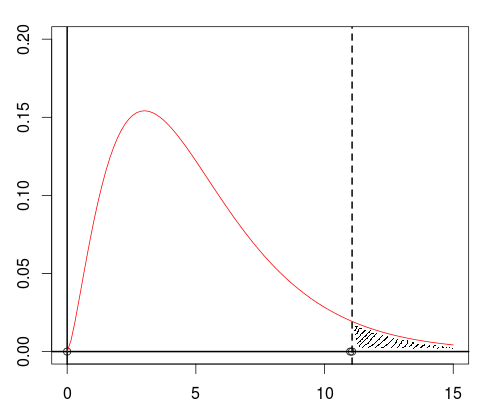
\includegraphics[scale=0.75]{img/ejemploEstadistica.png}

La raya vertical se sitúa en $x=11.07$, que es el valor que sale si se mira la tabla de la distribución $\chi^2$ con 5 grados de libertad (ver apéndice) y nivel de significación, por tanto, la zona sombreada es la región de rechazo de la hipótesis nula. Como ha salido T=11, no entramos dentro de esa región de rechazo (por poco) y no podemos rechazar la hipótesis nula.

\end{enumerate}
\end{example}

\begin{theorem}
Bajo $H_0$:
\[
\sum_{i=1}^k \frac{(O_i-E_i)^2}{E_i} \stackrel{d}{\rightarrow} \chi^2_{k-1} \text{ , si } n \rightarrow \infty
\]
\end{theorem}
\begin{proof}
\textcolor{blue}{Esta demostración es un poco liosa, si no la entendéis, a otra cosa (great pareado).}

Definimos los vectores aleatorios $\xi_1,...,\xi_n$ de la siguiente forma: $\xi_i=(0,...,\overbrace{1}^{(j)},...,0)' \in \mathbb{R}^k \Leftrightarrow x_i \in A_j$. Es decir cada $\xi_i$ va a ser un vector de 0's, salvo porque van a tener un 1 en una posición j. Esta posición j les identificará con la clase $A_j$. Tenemos que:
\[
\xi_1+...+\xi_n=(O_1,...,O_k)'
\]
Es decir, que su suma nos da un vector con las frecuencias de aparición de cada clase (Recordemos que 'k' es el número de clases). Por ejemplo, en el ejemplo del dado tendríamos que $\xi_1+...+\xi_6=(10,20,20,10,15,25)=(O_1,...,O_6)$

\textbf{Notación: } $p\equiv (p_1,...,p_k)'$. $np=(E_1,...,E_k)'$, entonces:
\[
(O_1-E_1,...,O_k-E_k)'=\left\{\sum_{i=1}^n(\xi_i)\right\}-np=n(\overline{\xi}-p)
\]

Definimos la matriz $\mathbb{P}$, que tiene rango k, se define con las probabilidades $p_i$ en la diagonal y 0 el resto de elementos:
\[
\mathbb{P}=\left(
\begin{array}{cccc}
p_1    & 0      & \cdots & 0 \\
0      & p_2    & \cdots & 0 \\
\vdots & \vdots & \ddots & \vdots \\
0      & 0      & \cdots & p_k \\
\end{array}
\right)
\]

Y cogiendo la raíz del estadístico de Pearson y sabiendo que $\sqrt{E_i}=\sqrt{np_i}$ nos queda:
\[
\left(\frac{O_1-E_1}{\sqrt{(E_1)}},...,\frac{O_k-E_k}{\sqrt{(E_k)}}  \right) = \mathbb{P}^{-1/2}\sqrt{n} (\overline{\xi}-\mathbb{P})
\]

Por otro lado: 
\[
v=(v_1,...,v_k) \rightarrow v'(\frac{v_1}{\lambda_1},...,\frac{v_k}{\lambda_k})
\]

Así, tomamos $\xi_1,...,\xi_n$ independientes y distribuidas como un vector $\xi$ tal que:
\[
\mathbb{E}(\xi)=p
\]
\[
V(\xi)=\mathbb{E}(\xi \xi') -pp' = \mathbb{P}-pp' \equiv \Sigma 
\]

$\mathbb{E}(\xi\xi')=\mathbb{P}$ ya que tenemos:
\[	ξ_r ξ_l =
	\begin{cases}
		0, & r≠l \\
		ξ_r^2 = ξ_r, & r=l \text{ ,pues } ξ_r \text{ es una Bernoulli}
	\end{cases}
\]

Por otra parte: 
\[
T=\sum_{i=1}^k \frac{(O_i-E_i)^2}{E_i} = \norm{p^{-1/2}\sqrt{n}(\xi-p)}^2
\]

Por el TCL:
\[
\sqrt{n}(\overline{\xi}-p) \stackrel{d}{\rightarrow} N_k(0, \Sigma) \implies \mathbb{P}^{-1/2}\sqrt{n}(\overline{\xi}-p) \stackrel{d}{\rightarrow} N_k(0, \mathbb{P}^{-1/2} \Sigma  \mathbb{P}^{-1/2}) 
\]
\[
\Rightarrow \norm{P^{-1/2} \sqrt{n} (\xi-p)}^2 \stackrel{d}{\rightarrow} \norm{Y}^2 \text{ con } Y \equiv N_k(0,\mathbb{P}^{-1/2} \Sigma  \mathbb{P}^{-1/2})
\]

Queda claro que $\mathbb{P}^{-1/2} Σ  \mathbb{P}^{-1/2}$ es simétrica, veamos que es idempotente:
\[\mathbb{P}^{-\frac{1}{2}} (\mathbb{P} - pp') \mathbb{P}^{-\frac{1}{2}} = I-\sqrt{p}\sqrt{p}'\]
donde $\sqrt{p}=(\sqrt{p_1}, …, \sqrt{p_2})'$.

\[
(I-\sqrt{p}\sqrt{p}')(I-\sqrt{p}\sqrt{p}') = I-2\sqrt{p}\sqrt{p}'+\sqrt{p}\underbrace{\sqrt{p}'\sqrt{p}}_{\sum p_i=1}\sqrt{p}'=I-\sqrt{p}\sqrt{p}'
\]

De el ejercicio 9 de la hoja 1 sabemos que una normal multivariante de media 0 y cuya matriz de covarianzas es simétrica e idempotente, cumple que su norma al cuadrado se distribuye como:
\[
\norm{Y}^2 \equiv \chi^2_{k-1}
\]
Los grados de libertad vienen de la traza de $\Sigma$, y de que $traza(I)=k$ y $traza(\sqrt{p}\sqrt{p'})=1$: 
\[
traza(\Sigma)=traza(I-\sqrt{p}\sqrt{p}') = traza(I) - traza(\sqrt{p}\sqrt{p}')=k-1
\]
\end{proof}

\section{Contraste de bondad de ajuste $\chi^2$ para hipótesis nula compuesta}

Problema: $X_1,...,X_n \stackrel{iid}{\sim} F$. Suponemos como hipótesis nula:
\[
H_0 : F \in \{F_{\theta}: \theta \in H \subset \mathbb{R}^r\}
\]

\textcolor{red}{La diferencia es que ahora la hipótesis nula que consideramos es que los datos van a seguir una distribución teórica $F_0$ que no está totalmente especificada, ya que va a depender de un parámetro. Por ello, decimos con palabras que:}

\textcolor{red}{La hipótesis nula es que los datos muestrales van a tener una función de distribución $F$, que va a ser igual a $F_{\theta}$, siendo $\theta$ el parámetro del que dependerá, el cual pertenece a un espacio paramétrico $H$}

Pasos:
\begin{enumerate}
\item Se definen k clases $A_1,...,A_k$. 

\item Se cuentan cuántos datos caen en cada clase (frecuencias observadas). Cada clase la llamaremos $O_i=\#\{j:X_j\in A_i\}$. Hasta aquí todo igual que antes.

\item Para estimar/calcular las frecuencias esperadas se sigue un método ligeramente diferente:

Se estima $\theta$ por el método de máximo verosimilutd. Sea $\hat{\theta}$ el EMV.

\textcolor{red}{explicar bien esto}

\item Se calculan las frecuencias esperadas estimadas bajo $H_0$: $\hat{E}_i=n\hat{p}_i$ con $i=1,...,k$ donde $\hat{p}_i = p_{\hat{\theta}}(A_i)$.

\item Calculamos el estadístico $\chi^2$ de Pearson:
\[
T=\sum_{i=1}^k \frac{(O_i-\hat{E}_i)^2}{\hat{E}_i}
\]

Ahora puedo elegir de todas las posibles distribuciones, aquella que más se parece. De modo que cabe esperar que T tienda a tomar valores menores que en el caso simple.

Además, al estimar r (\textcolor{red}{¿De dónde sale r? Es la dimensión del parámetro estimado??}) parámetros se introducen r nuevas restricciones sobre el vector $O_1,O_2,...,O_r$.

Se puede probar bajo condiciones de regularidad:
\[
\sum_{i=1}^k \frac{(O_i-\hat{E}_i)^2}{\hat{E}_i} \stackrel{d}{\rightarrow} \chi^2_{k-1-r} \text{ bajo } H_0 \text{ si } n \rightarrow \infty
\]

\item Se rechaza $H_0$ en la región crítica: $R=\{T>\chi^2_{k-1-r;\alpha}  \}$

Tal y como se ha hecho en el caso anterior.

\end{enumerate}

\begin{example}
Los bombardeos de Londres. El problema trata de estudiar los bombardeos que sufrío Londres entre 1944 y 1945. Se quería saber si los impactos sobre la ciudad de Londres eran en lugares aleatorios o estaban dirigidos a lugares concretos.

La fórmula de Poisson se ajusta bastante a un modelo de distribución aleatoria de impactos. Por tanto, tendríamos que estimar el parámetro $\lambda$ de la distribución de Poisson, que tiene por función de densidad:

$$ f(k,\lambda)=\frac{e^{-\lambda}\lambda^k}{k!} $$

Donde:
\begin{itemize}
\item k es el número de ocurrencias del evento o fenómeno (la función nos da la probabilidad de que el evento suceda precisamente k veces).

\item λ es un parámetro positivo que representa el número de veces que se espera que ocurra el fenómeno durante un intervalo dado. Por ejemplo, si el suceso estudiado tiene lugar en promedio 4 veces por minuto y estamos interesados en la probabilidad de que ocurra k veces dentro de un intervalo de 10 minutos, usaremos un modelo de distribución de Poisson con λ = 10×4 = 40.
\end{itemize} 
Dicho esto, vamos a seguir los pasos anteriormente detallados:



\begin{enumerate}
\item Se definen k clases $A_1,...,A_k$. En nuestro caso, las clases van a ser el número de impactos que ha habido en un cuadrado. Por tanto los cuadrados que pertenezcan a $A_1$ serán aquellos que han sufrido un único impacto.

\item Se cuentan cuántos datos caen en cada clase (frecuencias observadas). Cada clase la llamaremos $O_i=\#\{j:X_j\in A_i\}$. En nuestro caso tenemos: $O_0=229$, $O_1=211$, $O_2=93$, $O_3=35$, $O_4=8$ ($O_4$ es 4 o más impactos).


\item Para estimar/calcular las frecuencias esperadas se estima $\theta$ por el método de máximo verosimilutd. Sea $\hat{\theta}$ el EMV. En este caso, nuestro $\theta$ sera $\lambda$ y nuestro $\hat{\theta}$ será $\hat{\lambda}$, que será el parámetro de la distribución de Poisson:

$$ \hat{\lambda} = \frac{0\cdot229 + 1\cdot211+2\cdot93+3\cdot35+4\cdot7+5\cdot1}{576}=0.9323$$

\textcolor{red}{explicar por qué esto es el EMV, ya que en estadistica 1 hacíamos u lio increible pa sacarlo}

\item Se calculan las frecuencias esperadas $\hat{E}_i=n\hat{p}_i$ con $i=1,...,k$ donde $\hat{p}_i = p_{\hat{\theta}}(A_i)$. En nuestro caso:

$$\hat{E}_k = n\hat{p}_k = 576\cdot e^{-\hat{\lambda}\frac{\hat{\lambda}^k}{k!}}$$

Sustituimos $\lambda = 0.9323$ y $k=0,...,5$ y nos queda: $\hat{E}_0 = 226.74 $, $\hat{E}_1 = 211.34 $, $\hat{E}_2 = 98.54$, $\hat{E}_3 = 30.62$, $\hat{E}_4 = 8.71$.

\item Calculamos el estadístico $\chi^2$ de Pearson:
\[
T=\sum_{i=1}^k \frac{(O_i-\hat{E}_i)^2}{\hat{E}_i} = 1.0176
\]

Bajo $H_0$ tenemos que $T \equiv \chi^2_3$. El 3 sale de k=5 clases menos 1 parámetro estimado menos 1 como hacíamos antes.

\item Se rechaza $H_0$ en la región crítica: $R=\{T>\chi^2_{k-1-r;\alpha}  \}$

En nuestro caso, tomando $\alpha = 0.05$, tenemos: $$R=\{T>\chi^2_{3;\alpha} \} \rightarrow \{1.0176>7.815 \} \rightarrow \text{No se puede rechazar } H_0$$

Podemos calcular el p-valor mirando:
$$P\{\chi^2_3 > 1.0176\} = 0.797$$

Efectivamente, si miramos la tabla de la $\chi^2_3$, con $\alpha =0.797$, T valdría aproximadamente 1.
\end{enumerate}

\end{example}

\begin{example}
Ejemplo con R de los bombardeos:

Tenemos el siguiente comando para contrastes de bondad de ajuste de $\chi^2$:
\begin{verbatim}
chisq.test(datos,p=...)
\end{verbatim}

\begin{itemize}
\item datos: La muestra de la que disponemos.
\item p: Es el vector de probabilidades esperadas.
\item Por defecto, se contraste la hipótesis de que los datos siguen una distribución uniforme.
\item Se supone que bajo $H_0$ la distribución está completamente especificada (k-1 grados de libertad)
\end{itemize}
\textcolor{red}{Tengo anotado que R sólo funciona con hipótesis simples, y no compuestas, donde tenemos en cuenta eso?}

Exponemos el código a ejecutar y explicamos a continuación lo que hace:

\begin{verbatim}
res = c(seq(0,4),7)
obs = c(229,211,93,35,7,1)
n = sum(obs)
lambda = sum(res*obs)/n
prob = dpois(res,lambda)
esp = n*prob
\end{verbatim}

\begin{enumerate}
\item Guarda en \verb|res| un vector con las clases. Es decir, el número de impactos que ha habido en un cuadrado. Se obtiene:

\verb|res = 0 1 2 3 4 7|

\item Guarda en \verb|obs| un vector con el número de cuadrados de cada clase. Se obtiene:

\verb|obs = 229 211  93  35   7   1|

\item Guarda en \verb|n| el tamaño de la muestra, que es la suma de los elementos del vector \verb|obs|. Se obtiene \verb|n = 576|
\item Guarda en lambda el parámetro de la distribución de Poisson. Se obtiene \verb|lambda = 0.9322917|. Y sale de esta fórmula:
$$ \hat{\lambda} = \frac{0\cdot229 + 1\cdot211+2\cdot93+3\cdot35+4\cdot7+5\cdot1}{576}=0.9323$$
\item Guarda en \verb|prob| un vector con las probabilidades de aparición de cada clase, como la Poisson es una función de distribución discreta, que depende de dos parámetros, lo único que hacemos es sustituir en esta fórmula con $\lambda$ = \verb|lambda| y los valores de k = \verb|res|:
$$e^{-\hat{\lambda}\frac{\hat{\lambda}^k}{k!}}$$

Se obtiene:

\verb|prob = 3.9365e-01 3.6699e-01 1.7107e-01 5.3163e-02 1.2391e-02 4.7812e-05|

\item Guarda en \verb|esp| un vector con las esperanzas de cada clase. Se obtiene:

\verb|esp = 226.74272 211.39035  98.53873  30.62227   7.13722   0.02754|
\end{enumerate}

Continuamos agrupando las clases 4 y 5 es una sola clase, es decir, obteniendo una sola clase que serán los cuadrados con 4 o más impactos:

\begin{verbatim}
obs = c(obs[1:4], sum(obs[5:6]))
prob = c(prob[1:4], 1-sum(prob[1:4]))
esp = c(esp[1:4], n-sum(esp[1:4]))
\end{verbatim}

\begin{enumerate}
\item Obtenemos: \verb|obs = 229 211  93  35   8|
\item Obtenemos: \verb|prob = 0.393650 0.366997 0.171074 0.053163 0.015114|
\item Obtenemos: \verb|esp = 226.7427 211.3903  98.5387  30.6222   8.7059|
\end{enumerate}

Ahora vamos a dibujar el gráfico de barras:

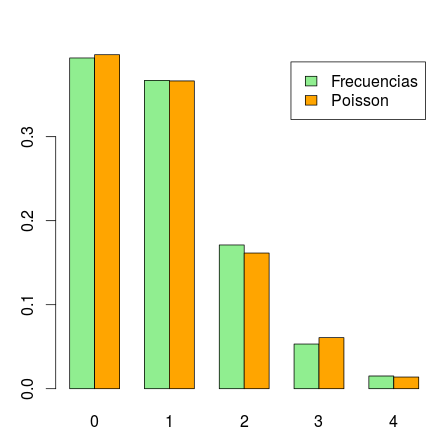
\includegraphics[scale=0.5]{img/contrasteba.png}

\begin{verbatim}
matriz = rbind(prob, obs/n)
rownames(matriz) = c('Frecuencias', 'Poisson')
barplot(matriz, beside=TRUE, names.arg=c(0:4),
 legend.text=TRUE, col=c('lightgreen','orange'))
\end{verbatim}

\begin{enumerate}
\item Guardamos en \verb|matriz| una matriz de dos filas, la primera son las probabilidades teóricas esperadas, la segunda las muestrales:
\begin{verbatim}
          [,1]      [,2]      [,3]       [,4]       [,5]
prob 0.3936506 0.3669971 0.1710742 0.05316368 0.01511444
     0.3975694 0.3663194 0.1614583 0.06076389 0.01388889
\end{verbatim}
\item Asignamos a la primera fila el nombre de 'Frecuencias' y a la segunda 'Poisson'.
\item Pintamos las barras con \verb|barplot|, con leyenda, y como nombre de cada par de barras ponemos 0,1,2,3 y 4, identificando las clases.
\end{enumerate}

Por último calculamos los valores importantes en un contraste, que son el p-valor, que es el mínimo valor de $\alpha$ a partir del cual podemos rechazar la hipótesis nula.

\begin{verbatim}
t = chisq.test(obs,p=prob)$statistic
pvalor = 1-pchisq(t,3)
\end{verbatim}

Obtenemos \verb|t =  1.017589  | y \verb|pvalor = 0.7969959|. El pvalor es muy alto, por tanto no podemos rechazar la hipótesis nula, es decir, no podemos rechazar que los datos proceden de una distribución de Poisson.  El nivel habitual de rechazo sería con $\alpha = 0.05$ que implica que si lo rechazamos tenemos un $5\%$ de posibilidades de equivocarnos. Si quisiéramos rechazar con un $\alpha = 0.79$, tendríamos una probabilidades del $79\%$ de equivocarnos.



\end{example}



\section{Contraste de bondad de ajuste de Kolmogorov-Smirnov}
Sea $X_1,...,X_n \stackrel{iid}{\sim} F$. Definimos la función de distribución empírica, correspondiente a $X_1,...,X_n$ como:

$$ F_n(x)=\frac{1}{n}\#\{i: X_i \leq x\} $$

Es una función de distribución constante a trozos, y con saltos de magnitud $\frac{1}{n}$ en cada valor muestral de $X_i$. Aunque ponga $F_n$, solo hay una para la muestra entera (ya que las variables aleatorias están idénticamente distribuidas), sólo se pone $F_n$ porque depende directamente del número de elementos de la muestra.

Consideramos como hipótesis nula $H_0: F=F_0$. Siendo $F_0$ una distribución previamente especificada

Así, $F_n$ es un estimador de la verdadera distribución F. Que como toda distribución se define como $F(X)=P(X\leq x)$.

\begin{example}
Consideramos una muestra con 3 elementos: $X_1=1, X_2=4, X_3=6$. Ahora, para que sea más fácil construir la función de distribución ordenamos la muestra y nos queda:
$$ X_{(1)}=1 \text{, }X_{(2)}=4 \text{, }X_{(3)}=6 \rightarrow \text{Estos son los estadísticos de orden}$$

Por tanto, la función de distribución queda:

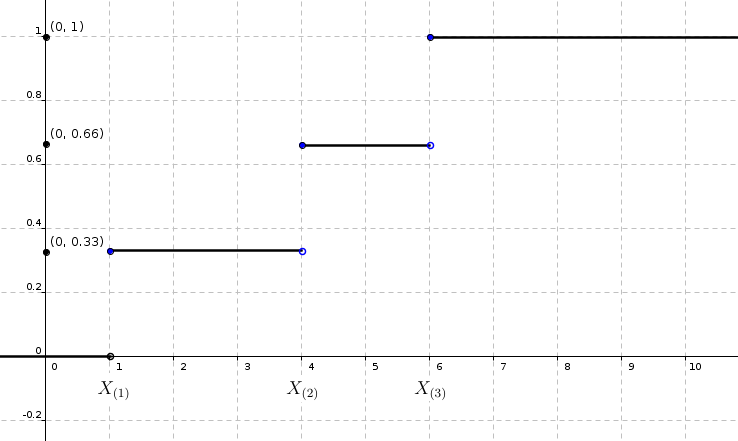
\includegraphics[scale=0.5]{img/contrasteks.png}

Y es bastante razonable. Por ejemplo $P(X=1) = F(1^+)-F(1^-)=\frac{1}{3}-0=\frac{1}{3}$. Algo similar ocurre con $P(X=4) = P(X=6) = \frac{1}{3}$. Lo cual es razonable si nos limitamos únicamente a observar la muestra. Además, para el resto de valores de X, la probabilidad es 0: $P(X=2)=F(2^+)-F(2^-) = \frac{1}{3}-\frac{1}{3}=0$
\end{example}

\begin{obs}
\begin{enumerate}
\item Esta observación sale de sustituir en las fórmulas con las definiciones que hemos dado. Sabiendo que la esperanza de una binomial es $\mathbb{E}\Big(B(n,p)\Big)=np$ $$nF_n(x) = \#\{i:X_i\leq x \} \equiv B(n, F(x))  \Rightarrow \mathbb{E}\Big[F_n(X)\Big] = \frac{1}{n} n F(x) = F(x)$$
\item Con el mismo razonamiento, pero sabiendo que si $X \sim B(n,p)$, entonces $Var(X)=np(1-p)$:
$$ Var(F_n(X))=\frac{1}{n^2}nF(x)(1-F(x)) \stackrel{n \rightarrow \infty}{\rightarrow} 0$$
\item Como consecuencia:
$$ F_n(X) \stackrel{P}{\rightarrow} F(X)$$

Convergencia en probabilidad o en medida: Si $\forall \epsilon >0$, $\lim_{n \rightarrow \infty}P(\abs{X-X_n}\geq \epsilon)=0$.
\end{enumerate}
\end{obs}
De hecho, se cumple que (lema de Glivenko-Cantelli):
$$\norm{F_n-F}_{\infty} = \sup\abs{(F_n(X)-F(x)} \stackrel{c.s.}{\rightarrow} 0$$

Si $H_0: F=F_0$ fuese cierta, se espera que $D_n = \norm{F_n-F_0}_{\textcolor{red}{\infty}}$ sea pequeño ($D_n$ es el estadístico de Kolmogorov-Smirnov). La idea es rechazar en la región $R=\{D_n > C\}$, para un valor c tal que $P_{H_0}(D_n > c)=\alpha$, donde $\alpha$ es el nivel de significación.

\textcolor{red}{\textbf{Importante:}la distribución bajo $H_0$ de $D_n$ es la misma para cualquier distribución continua $F_0$. El valor de c en la región crítica es el mismo para cualquier distribución continua $F_0$ y esta tabulado. $F_0$ es la distribución teórica a la que queremos ver si pertenecen los datos. Mientras que $F=F_n$ que es la empírica.}

\begin{prop}
Si una v.a. X tiene distribución continua (\textcolor{red}{Continua por la derecha en todo caso}) $F_0$, entonces la v.a. $F_0(X) \sim U(0,1)$ (Uniforme en (0,1)).
\end{prop}
\begin{proof}
Queremos ver que $P(F_0(X)\leq u)=u$ $\forall u \in [0,1]$ (que es lo que ocurriría si $F_0$ siguiera una distribución uniforme entre 0 y 1).

Así, sea $F_0$ continua, entonces existe un x tal que $F_0(x)=u$. Y tendríamos que:
$$ P(F_0(X)\leq u) = P(F_0(X)\leq F_0(x)) $$

Ahora sabiendo que la función de distribución es monótona creciente (m.c.), del primer miembro nos quitamos $F_0(X)\leq F_0(X)$ y del segundo, el menor o igual, ya que si $X>x$ solo puede ser que $F_0(X)= F_0(X)$:
$$\{ F_0(X)\leq F_0(x) \} = \{ F_0(X)\leq F_0(x), X \leq x\} \cup \{ F_0(X)\leq F_0(x), X > x\} = $$
$$ =  \{ X \leq x\} \cup \{ F_0(X) \underbrace{=}_{m.c.} F_0(x), X > x\}$$

Y, basándonos en que $F_0(X)=P(X \leq x)=u$ y en que la probabilidad es 0 en un trozo donde la función de distribución es constante, nos qued: 
$$P(F_0(X)\leq F_0(x)) = P(X \leq x) + P(F_0(X) = F_0(x), X \geq x) = F_0(X) + 0 = u$$
\end{proof}

\begin{obs}
Existe un recíproco de la proposición: Si $U \sim U(0,1) \Rightarrow F^{-1}(U) \sim F$. \textcolor{red}{Explicar mejor este recíproco}
\end{obs}

La $D_n$ de la que estábamos hablando antes de meternos en la proposición se conoce como:

\begin{defn}[Estadístico Kolmogorov-Smirnov]
	\[D_n = \max \left\{ 0, \max_{i=1,…,n} \left( \frac{i}{n} - F_0(x_{(i)}) \right), \max_{i=1,…,n} \left(F_0(x_{(i)}) - \frac{i-1}{n})\right) \right\}\]
\end{defn}

Y a continuación vamos a demostrar por qué tiene la expresión que aparece en la definición.
\begin{proof}

$$ D_n = \max \left\{ \sup_{x\in\mathbb{R}} \Big( F_n(x)-F_0(x)\Big), \sup_{x\in\mathbb{R}} \left( F_0(x)-F_n(x)\right) \right\} $$

Si representamos los estadísticos de orden de la muestra en una recta, y llamamos a $X_{(0)}=-\infty$ y $X_{(n+1)}=\infty$:

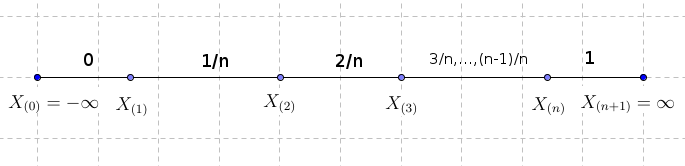
\includegraphics[scale=0.5]{img/contrasteks2.png}

Nos queda que si x está entre $X_{(i)}$ y $X_{(i+1)}$, entonces $F_n(x)=\frac{i}{n}$.

Desarrollando el primer término de $D_n$ nos queda:
$$ \sup_{x\in\mathbb{R}} \Big( F_n(x)-F_0(x)\Big) = \max_{i=0,...,n} \Bigg(\sup_{x\in(X_{(i)},X_{(i+1)})} \Big( F_n(x)-F_0(x)\Big) \Bigg) = $$

$$ = \max_{i=0,...,n} \Big( \frac{i}{n} - F_0(X_{(i)}) \Big) = \max\Big\{ 0, \max_{i=1,...,n} \Big( \frac{i}{n} - F_0(X_{(i)}) \Big) \Big\}$$

\textcolor{red}{Explicar por qué es $\frac{i}{n}$} % Jorge: Es por definición de la función de distrib. empírica.

Desarrollando el segundo término nos queda:
\[\sup_{x∈ℝ}\left( F_0(x) - F_n(x) \right) = \max_{j=0,…,n} \left( \sup_{x∈(x_{(j)},x_{(j+1)})} \left( F_0(x) - F_n(x) \right) \right) =\]

\[= \max_{j=0,…,n} \left( F_0(x_{(j+1)}) - \frac{j}{n} \right) \underbrace{=}_{i=j+1} \max_{i=1,…,n+1} \left( F_0(x_{(i)}) - \frac{i-1}{n} \right) =  \]
$$ = \left\{ 0, \max_{i=1,...,n} \left( F_0(X_{(i)}) - \frac{i-1}{n} \right) \right\} $$

\textcolor{red}{Explicar por qué es $\frac{i-1}{n}$}

Por tanto, finalmente nos queda:
$$ D_n =  \norm{F_n-F_0}_{\infty} = \max\Big\{ 0, \max_{i=1,...,n} \Big( \frac{i}{n} - F_0(X_{(i)}) \Big) , \max_{i=1,...,n} \Big( F_0(X_{(i)}) - \frac{i-1}{n} \Big)$$

Por tanto concluimos que $D_n$ depende de $F_0$ a través de los valores de $F_0(X_{(1)}), F_0(X_{(2)}),...,F_0(X_{(n)})$. Si tengo una muestra de $X_1,...,X_n \stackrel{iid}{\sim}F_0$, entonces $F_0(X_1),...,F_0(X_1) \stackrel{iid}{\sim} U(0,1)$. Ordenándolos los elementos: $X_{(1)}\leq...\leq X_{(n)}$, entonces $F_0(X_{(1)})\leq...\leq F_0(X_\textbf{{(n)}}) \stackrel{iid}{\sim} U(0,1)$. Que son los estadísticos de orden de una muestra de tamaño n, de variables aleatorias iid, que siempre van a seguir una distribución de una $U(0,1)$ para toda $F_0$ continua.

\textbf{Notación}
$$D_n^+=\max_{i=0,...,n} \Big( \frac{i}{n} - F_0(X_{(i)}) \Big)$$
$$D_n^-= \max_{i=0,...,n} \Big( F_0(X_{(i)}) - \frac{i-1}{n} \Big)$$

\end{proof}

\begin{example}
Ejemplo con R:

Tenemos el siguiente comando para contrastes de bondad de ajuste de Kolmogorov-Smirnov:
\begin{verbatim}
ks.test(datos,distribucion,parametros)
\end{verbatim}

\begin{itemize}
\item \verb|datos|: La muestra de la que disponemos.
\item \verb|distribucion|: Distribución bajo $H_0$. Es la distribución que creemos teórica de los datos, la que hemos llamado $F$. (Por ejemplo, $pnorm$).
\item \verb|parametros|: Parámetros de la distribución $F$. 
\end{itemize}
Vamos a probar a usar los datos 'Kevlar'. Corresponden al tiempo hasta el fallo (en horas) de 101 barras de un material utilizado en los transbordadores espaciales.

Obtenemos los datos de \url{http://www.uam.es/personal_pdi/ciencias/acuevas/docencia/estI/Datos-kevlar.txt}. Los metemos en un archivo de texto $kevlar.txt$.

Ejecutamos:

\begin{verbatim}
kev = scan('kevlar.txt')

boxplot(kev)

hist(kev)

plot(ecdf(kev), verticals=TRUE, do.points=FALSE)
curve(pexp(x), add=TRUE, col='red')
\end{verbatim}
 
Y obtenemos estas tres figuras:

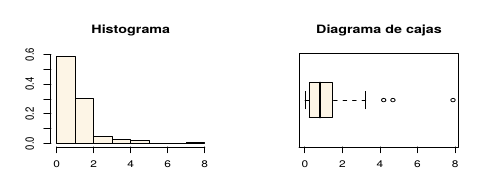
\includegraphics[scale=0.8]{img/contrasteks3.png}
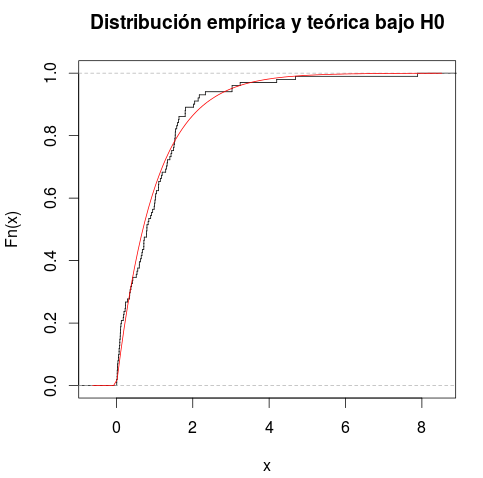
\includegraphics[scale=0.5]{img/contrasteks4.png}

En esta última observamos perfectamente la función $F_n$ constante a trozos con valores $\frac{1}{n}$. Hemos contrastado la muestra con la hipótesis nula de que los datos siguen una distribución exponencial de parámetro $\lambda = 1$. (esta es la recta roja que sale con $pexp(x)$).

Por último ejecutamos:
\begin{verbatim}
ks.test(kev,pexp)
\end{verbatim}

Y obtenemos:
\begin{verbatim}
data:  kev
D = 0.087038, p-value = 0.4286
alternative hypothesis: two-sided
\end{verbatim}

Si ejecutamos \verb|ks.test(kev, pnorm)$statistic|, obtenemos solo el valor del estadístico: \verb|0.08703787| 

\end{example}

\begin{example}
Contrastar a nivel $\alpha=0.01$ si la muestra $X_1=16, X_2=8, X_3=10, X_4=12, X_5=6$ procede de una distribución exponencial de media $11.5$.

Sea X una v.a con distribución exponencial, tiene función de distribución:
$$F_0(X) = 1-e^{-\lambda x} \text{ si x } \geq 0$$

Y sabemos que $\mathbb{E}(X)=\frac{1}{\lambda}$. De esto, sacamos que en nuestro caso $\lambda = \frac{1}{11.5}$ 

\begin{tabular}{|c|c|c|c|c|}
\hline
 $X_{(i)}$ & i/n & $F_0(X_{(i)})$ & $D_n^+$ & $D_n^-$ \\
\hline
6 & 0.2 & 0.41 & -0.21 & 0.41 \\
\hline
8 & 0.4 & 0.5 & -0.1 & 0.3 \\
\hline
10 & 0.6 & 0.58 & 0.02 & 0.18 \\
\hline
12 & 0.8 & 0.65 & 0.15 & 0.05 \\
\hline
16 & 1 & 0.75 & 0.25 & -0.05 \\
\hline
\end{tabular}

Así, nos queda que $D_n = 0.41$.

Y mirando en la tabla de la exponencial con nivel de significación $\alpha = 0.01$, tenemos que c= \textcolor{red}{terminar ejercicio}

\end{example}

\section{Gráficos de probabilidad}
Sean $X_1,...,X_n \stackrel{iid}{\sim} F \Rightarrow F(X_1),...,F(X_n) \stackrel{iid}{\sim} U(0,1)$. Si ordenamos las F nos quedan los estadísticos de orden de una $U(0,1)$: $F(X_{(1)}),...,F(X_{(n)})$.

Por tanto, si tengo una muestra de tamaño 2, entonces la media sería que F del dato más pequeño $F(X_{(1)})$ sea $\frac{1}{3}$ y que el dato más grande $F(X_{(2)})$ sea $\frac{2}{3}$. Ya que hemos estimado que F sigue una distribución uniforme en $[0,1]$.

De la misma forma, si hay n datos, la media sería que el dato mínimo se encuentre en $\frac{1}{n+1}$ y el dato máximo en $\frac{n}{n+1}$.

En definitiva, tenemos que la media del valor de F del dato i-ésimo es:
$$\mathbb{E}(F(X_{(i)}) \approx \frac{i}{n+1}$$

Es decir, tendríamos que $F(X_{(i)}) \approx \frac{i}{n+1}$ y por tanto, debería ocurrir que $X_{(i)} \approx F^{-1}(\frac{i}{n+1})$. Si esto ocurre, tendríamos una gráfica que representaría la recta y=x, en el eje de ordenadas tendríamos $F^{-1}(\frac{i}{n+1})$ y en el eje de abscisas tendríamos $X_{(i)}$. La idea es que si esto ocurre los datos vienen de una normal, es decir: $X_1,...,X_n \stackrel{iid}{\sim} F=N(\mu, \sigma)$.

Además, sea $\Phi \sim N(0,1)$. Sea $F(X) = \Phi(\frac{x-\mu}{\sigma})$ entonces:
$$ X_{(i)} = F^{-1}\Big(\frac{i}{n+1}\Big) = \sigma \Phi^{-1}\Big(\frac{i}{n+1}\Big)+ \mu $$

Se representa la gráfica:
$$ \bigg( X_{(i)}, \Phi^{-1}\Big(\frac{i}{n+1}\Big) \bigg)$$

Si la gráfica es una recta, no necesariamente de pendiente 1, quiere decir que los datos son normales.

Aquí tenemos 12 ejemplos:

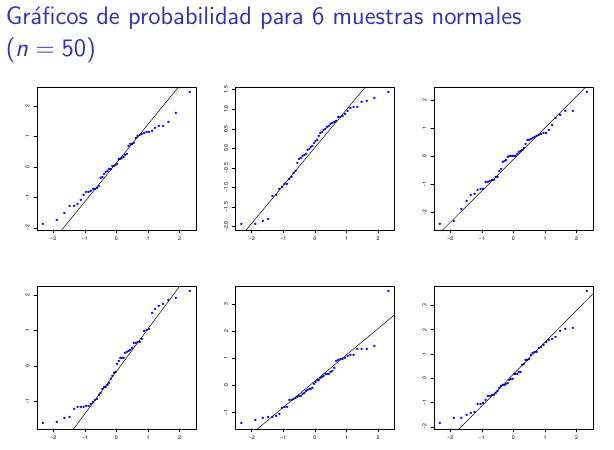
\includegraphics[scale=0.6]{img/graficos1.png}

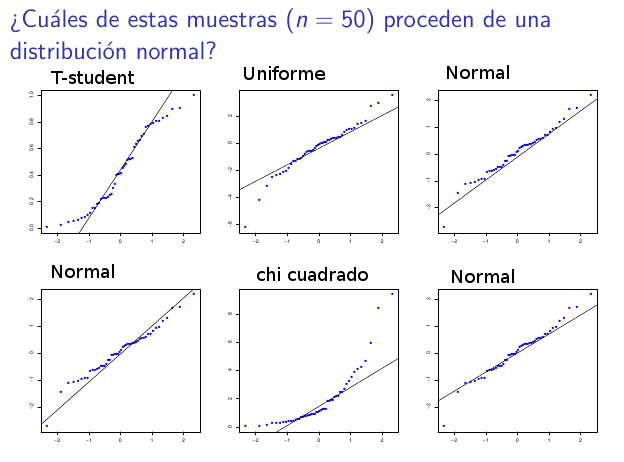
\includegraphics[scale=0.6]{img/graficos2.png}

\section{Contraste $\chi^2$ de homogeneidad}
Sean un conjunto de muestras tomados de diferentes lugares o contextos $M_1,...,M_p$. Cada conjunto de muestras seguirá una distribución $F_1,..,F_p$.

\begin{align*}
M_1 \equiv & X_{11} .... X_{1\cap 1} \stackrel{iid}{\sim} F_1 \\
& \vdots \\
M_p \equiv & X_{p1} .... X_{p\cap p} \stackrel{iid}{\sim} F_p
\end{align*}

\textcolor{red}{lo de la intersección en $X_{p\cap p}$ que es??}
\textcolor{blue}{No es un símbolo de intersección sino la letra $n$, refiriendose a que el tamaño muestral de cada muestra puede ser diferente: $X_{1n_1},X_{1n_2},...,X_{1n_p}$}

Consideraremos como hipótesis nula: $H_0: F_1=...=F_p$. Es decir, queremos ver si las muestras tomadas de diferentes lugares siguen la misma distribución.

Dividimos los datos de cada conjunto de muestras en clases $A_1,...,A_k$, todos los conjuntos $M_1,...,M_p$ tendrán los mismos tipos de clases. Y consideramos las frecuencias observadas: $O_{ij}=$ nº de datos de $M_j$ en $A_i$.

Llamamos tabla de contingencia a la siguiente tabla:

\begin{tabular}{cccc}
& $M_1$ & ... & $M_p$ \\
$A_1$ & $O_{11}$ &  & $O_{1p}$ \\
\vdots &  & $O_{ij}$ &  \\
$A_k$ & $O_{k1}$ &  & $O_{kp}$ \\
\end{tabular}

Cada elemento $O_{ij}$ de la tabla es el número de muestras de una clase para cada conjunto de muestras. Queremos estimar este valor mediante una binomial (\textcolor{red}{por que?} \textcolor{blue}{ Porque una binomial Bin(n,p) modela el número de éxitos en n experimentos independientes donde la probabilidad de éxito es p. En este caso, $O_{ij}$ es el número de observaciones de la muestra j que caen en la clase i, que es lo mismo que el numero de éxitos entre nj observaciones (las que hay en la muestra j) que caen en la clase i }). Así:
$$ O_{ij,H_0} \equiv B(n_j, p_i)  \text{ con } p_i=P_{H_0}(A_i)$$

Pero desconocemos este valor $P_{H_0}(A_i)$, por lo que lo tenemos que estimar.

Llamamos $E_ij =n_j p_i$ frecuencia esperada bajo $H_0$.

Realizamos la siguiente operación \textcolor{red}{El por qué es aún un misterio}:
$$ \sum_j \underbrace{\sum_i \frac{(O_{ij}-E_ij)^2}{E_{ij}}}_{\chi^2_{k-1}} \stackrel{d}{\rightarrow} \underbrace{\chi^2_{p(k-1)}}_{p\chi^2_{k-1}} $$

Queremos estimar $p_1,...,p_k$:
$$\hat{p}_i=\frac{\sum_{j=1}^p O_{ij}}{n}$$

Con $n=n_1+...+n_p$, como tenemos homogeneidad, es como si tuviéramos $n_1+n_2+...+n_p$ datos en total. 

Ahora podemos calcular la esperanza estimada:
$$\hat{E}_{ij} = n_j \hat{p}_i=n_j \cdot \frac{\sum_j O_{ij}}{n}$$

\textbf{Notación:} 
\begin{itemize}
\item $\sum_j O_{ij} = O_{i\cdot}$
\item $\sum_j O_{ij} = n_j =  O_{\cdot j}$
\end{itemize}
Por tanto:
$$\hat{E}_{ij} = \frac{O_{i\cdot} O_{\cdot j}}{n}$$

Y ahora hacemos una tabla parecida a la anterior pero con las esperanzas estimadas:

\begin{tabular}{cccc}
& $M_1$ & ... & $M_p$ \\
$A_1$ & $\hat{E}_{11}$ &  & $\hat{E}_{1p}$ \\
\vdots &  & $\hat{E}_{ij}$ &  \\
$A_k$ & $\hat{E}_{k1}$ &  & $\hat{E}_{kp}$ \\
\end{tabular}

Ahora con los estimadores obtenidos:
$$ \sum_i \sum_j \frac{(O_{ij}-\hat{E}_{ij})^{\textcolor{red}{2}}}{\hat{E}_{ij}} \stackrel{d}{\rightarrow} \chi^2_{(p-1)(k-1)} $$

Como podemos observar, la $\chi^2$ no es de $p(k-1)$ como antes sino que es de $p(k-1)-(k-1)$, los últimos $k-1$ son el nº de parámetros estimados. Ya que estimamos $\hat{p}_1,...,\hat{p}_k$, pero con la condición $\hat{p}_1+...+\hat{p}_k  1$.

La región de rechazo quedaría:
$$ R=\{T > \chi^2_{(k-1)(p-1),\alpha}\}$$

\begin{obs}
Se puede comprobar que:
$$ T = \sum_{i=1}^k \sum_{j=1}^p \frac{O_{ij}}{E_{ij}}-n$$

\textcolor{red}{Y antes dónde habíamos definido T??}
\end{obs}

\begin{example}
Tenemos 3 muestras, una de España, otra de Italia y otra de Francia, todas de tamaño $n=100$.Las clases son 'no fumadores' (NF), 'fumadores ocasionales' (FO) y 'fumadores habituales' (FH).

Tenemos la siguiente tabla de contingencia:

\begin{tabular}{ccccc}
& $M_1=$España & $M_2=$Italia & $M_3=$Francia & \\
$A_1=$NF & $O_{11}=30$ & $O_{12}=15$ & $O_{13}=20$ & $O_{1\cdot}=65$ \\
$A_2=$FO & $O_{21}=50$ & $O_{22}=40$ & $O_{23}=50$ & $O_{2\cdot}=140$ \\
$A_3=$FH & $O_{31}=20$ & $O_{32}=45$ & $O_{33}=30$ & $O_{3\cdot}=95$ \\
& $O_{\cdot1}=n_1=100$ & $O_{\cdot2}=n_2=100$ & $O_{\cdot3}=n_3=100$ & 300 \\
\end{tabular}

Recordamos la fórmula de la esperanza estimada:
$$\hat{E}_{ij} = n_j \cdot \frac{\sum_j O_{ij}}{n} = \frac{O_{i\cdot} O_{\cdot j}}{n}$$

Vamos a calcular la esperanza estimada $\hat{E}_{12}$ es decir, la de Italia y no fumadores:

$$\hat{E}_{12} = n_2 \hat{p}_1 = n_2 \cdot \frac{\sum_{j=1}^3 O_{1j}}{n} = 100 \cdot \frac{30+15+20}{300} = 21,\stackrel{\frown}{6}$$

Así, la tabla de esperanzas quedaría:

\begin{tabular}{ccccc}
& España & Italia & Francia & \\
NF & $\hat{E}_{11}=21,\stackrel{\frown}{6}$ & $\hat{E}_{12}=21,\stackrel{\frown}{6}$ & $\hat{E}_{13}=21,\stackrel{\frown}{6}$ & 65 \\
FO & $\hat{E}_{21}=46,\stackrel{\frown}{6}$ & $\hat{E}_{22}=46,\stackrel{\frown}{6}$ & $\hat{E}_{23}=46,\stackrel{\frown}{6}$ & 140 \\
FH & $\hat{E}_{31}=31,\stackrel{\frown}{6}$ & $\hat{E}_{32}=31,\stackrel{\frown}{6}$ & $3\hat{E}_{33}=31,\stackrel{\frown}{6}$ & 95 \\
& 100 & 100 & 100 & 300 \\
\end{tabular}

Ahora calculamos el estadístico T:
$$ T = \sum_{i=1}^k \sum_{j=1}^p \frac{O_{ij}}{E_{ij}}-n = $$
$$\frac{30}{21,\stackrel{\frown}{6}} + \frac{15}{21,\stackrel{\frown}{6}} + \frac{20}{21,\stackrel{\frown}{6}} + \frac{50}{46,\stackrel{\frown}{6}} + \frac{40}{46,\stackrel{\frown}{6}} +
\frac{50}{46,\stackrel{\frown}{6}} +
\frac{20}{31,\stackrel{\frown}{6}} +
\frac{45}{31,\stackrel{\frown}{6}} +
\frac{30}{31,\stackrel{\frown}{6}} = 9$$

\textcolor{red}{No sale lo esperado, revisar y terminar}

La región de rechazo es:
$$ R=\{T > \chi^2_{(k-1)(p-1),\alpha}\}$$

En nuestro caso, suponiendo un nivel de significación $\alpha=0.05$:
$$ R=\{T > \chi^2_{(3-1)(3-1),0.05}\} \Rightarrow R=\{T > \chi^2_{4,0.05}\} \Rightarrow  R=\{T > 9.488\}$$
\end{example}

\section{Contraste Kolmogorov-Smirnov de homogeneidad}
Este contraste sólo es válido para dos muestras, y para distribuciones continuas. Al igual que antes queremos ver que las dos muestras tienen la misma distribución.

Así, tenemos $X_1,...,X_n \stackrel{iid}{\sim} F$ y $Y_1,...,Y_n \stackrel{iid}{\sim} G$, con F y G continuas. La hipótesis nula será $H_0: F=G$, es decir, los datos de la primera muestra están distribuidos con la misma función de distribución que los datos de la segunda muestra.

Para ello calculamos el estadístico K-S para dos muestras:

$$D_{n,m} = \norm{F_n -G_m}_{\infty} = \sup_{x \in \mathbb{R}} \abs{F_n(x)-G_m(x)}  $$

Bajo $H_0$ la distribución $D_{n,m}$ no depende de F=G y está tabulada.
$$ R=\left\{D_{n,m} > C_{\alpha}\right\} $$

\section{Contraste $\chi^2$ de independencia}
Sea $(X_1, Y_1),...,(X_n, Y_n) \stackrel{iid}{\sim} F$. Y sea la hipótesis nula $H_0 :$ X e Y son independientes.

\textcolor{red}{terminar esto en otro momento que no lo veo muy claro}


\chapter{Regresión}
El objetivo de la regresión es predecir una/s variable/s en función de la/s otra/s.


\section{Regresión lineal}

Observamos dos variables, X e Y , el objetivo es analizar la relación existente entre ambas, de forma que podamos predecir o aproximar el valor de la variable Y a partir del valor de la variable X.

\begin{itemize}
\item La variable Y se llama variable respuesta.
\item La variable X se llama variable regresora o explicativa.
\end{itemize}

Por ejemplo:
\begin{center}
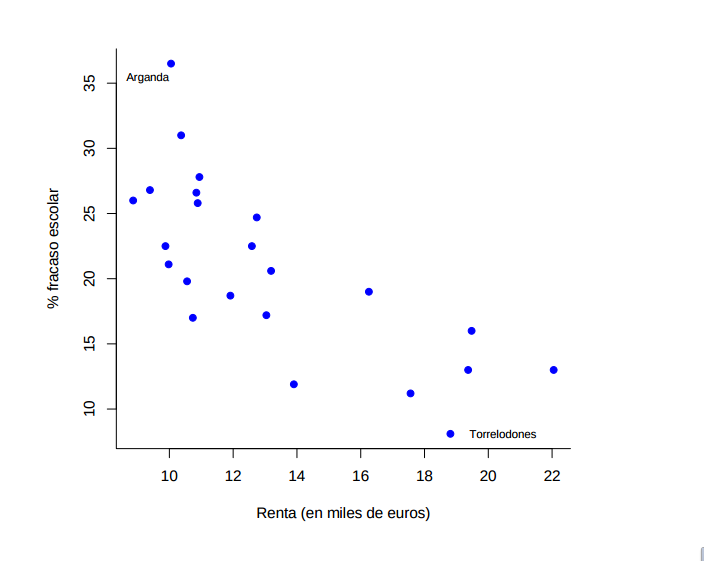
\includegraphics[scale=0.5]{img/RentaVsFracaso.png}
\end{center}

Queremos predecir el fracaso escolar en función de la renta. La variable respuesta es el fracaso escolar, mientras que la variable regresora es la renta.

\subsection{Regresión lineal simple}

Frecuentemente existe una relación lineal entre las variables. En el caso del fracaso escolar,queremos construir una recta $Y_i = β_0 X_i + β_1\; i=1,...,n$ que minimice el error.

El problema es estimar los parámetros $β_0,β_1$. Una manera de hacer esto es:

\subsubsection{Recta de mínimos cuadrados}

\begin{defn}[Recta de mínimos cuadrados]
Estimando $β_i$ por $\hat{β_i}$ obtenemos: \[\hat{Y_i} = \hat{β}_0 + \hat{β}_1 x_i\]

La reca viene dada por los valores $\hat{β_0}, \hat{β_1}$ para los que se minimiza el error cuadrático, es decir:
\[\sum_{i=1}^n \left(Y_i - \hat{Y_i}\right)^2 =  \sum_{i=1}^n \left[ Y_i - (\hat{β_0} + \hat{β_1}x_i) \right]^2\]
\end{defn}

\begin{example}
\begin{center}
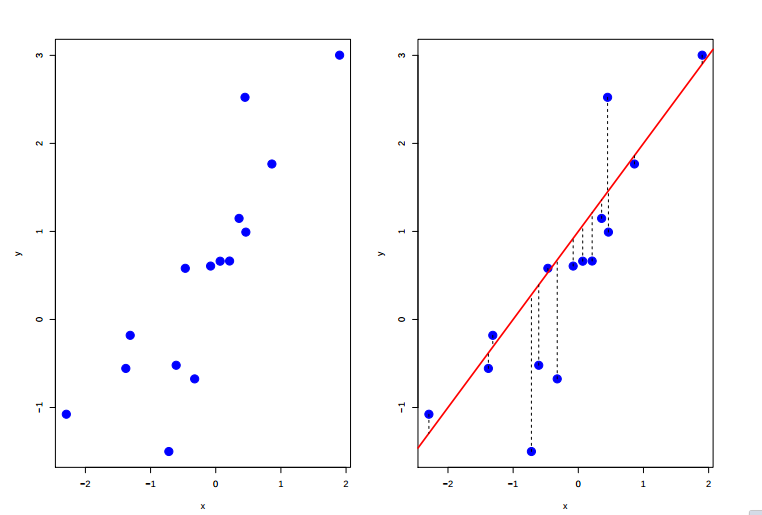
\includegraphics[scale=0.6]{img/ejemploRectaRegresionLineal.png}
\end{center}
\end{example}

\paragraph{Cómo calcular la pendiente} de la recta de mínimos cuadrados.


Vamos a ver unas pocas maneras de calcular la recta de mínimos cuadrados.

\begin{itemize}

	\item El sistema habitual:

	\[ \hat{β_1} = \frac{\sum_{i=1}^n(x_i - \bar{x})(Y_i - \bar{Y})}{\sum_{i=1}^n (x_i - \bar{x})^2} = \frac{S_{xy}}{S_{xx}} \]
	Donde
		\[S_{xy} = \sum_{i=1}^n(x_i - \bar{x})(Y_i - \bar{Y}) \]
		\label{Ssubxx}
		\[S_{xx} = \sum_{i=1}^n (x_i - \bar{x})^2\]
	\subitem \[β_0 = \bar{Y} - β_1\bar{x}\]

	\textbf{Entonces:}
	\[\text{recta} \equiv y - \bar{y} = \frac{S_{xy}}{S_{xx}}(x - \bar{x} ) \]

	\item Mínimos cuadrados como promedio de pendientes:
	\label{rmc::promediopendientes}
	\[
	\hat{β_1} = \frac{S_{xy}}{S_{xx}} = \sum_{i=1}^n \frac{(x_i - \bar{x})^2}{S_{xx}} \left( \frac{(Y_i - \bar{Y})}{x_i - \bar{x}} \right) = \sum_{i=1}^n ω_i \left( \frac{(Y_i - \bar{Y})}{x_i - \bar{x}} \right)
	\]

	Vemos que hemos ponderado la pendiente de cada recta que une cada punto con la media. Este peso es mayor cuanto mayor es la distancia \textbf{horizontal}.

	\item Mínimos cuadrados como promedio de respuestas:

	\[
	\hat{β_1} = \frac{\sum_{i=1}^n  (x_i - \bar{x}) (Y_i - \bar{Y})}{S_{xx}} = \sum α_i Y_i
	\]
	Es interesante ver unas propiedades de estos $α_i$
	\begin{prop}


		\begin{itemize}
			\item[] $\sum α_i = 0$
			\item[] $\sum α_ix_i = 1$
			\item[] $\sum α_i^2 = \frac{1}{S_{xx}}$
		\end{itemize}

	\end{prop}
	\begin{proof}
	\textcolor{red}{Por hacer}
	\end{proof}

\end{itemize}


\begin{defn}[Residuo]
En una recta de mínimos cuadrados: Sea $y_i = β_1x_i - β_0$ y sea $\hat{y}_i = \hat{β}_1x_i - \hat{β}_0$, llamamos residuo a $$e_i = y_i - \hat{y}_i$$

Los residuos cumplen:

\[
\sum_{i=1}^n e_i = 0
\]

Esto es intuitivo, ya que los errores se compensan y además es una buena propiedad.
\end{defn}



\begin{prop}
Sean $\{e_i\}$ una variable aleatoria que cumple \footnote{Se ha utilizado la $e$ porque es útil en cuanto a los residuos de la recta de mínimos cuadrados}:
\[\sum e_i = 0\]

Entonces:
\[\sum e_i x_i = 0 \implies \cov(e,x) = 0\]
\end{prop}

\begin{proof}
\[\sum (e_i - \vec{µ}) x_i = \sum (e_i - \vec{µ}) (x_i - \vx) \]
Por otro lado:

\[
\sum e_ix_i = \sum e_ix_i - \vx \sum e_i = \sum e_i(x_i - \vx)
\]
\end{proof}


\begin{example}
\[
\sum (x_i - \vx)(y_i -\vy) = \sum (x_i - \vx)y_i - \sum \vy\sum(x_i - \vx) \overset{(1)}{=} \sum(x_i - \vx y_i)
\]
\[
(1) \to \sum(x_i - \vx) = 0
\]
\end{example}

Esto tiene la siguiente explicación ``intuitiva'': La recta de mínimos cuadrados contiene toda la información lineal que $X$ puede dar sobre $Y$ (debido a que la covarianza entre los residuos y $X$ es 0).


\subsubsection{Fallos de la recta de mínimos cuadrados}

Vamos a ver un par de ejemplos ilustrativos:

\begin{example}[Sobre los datos atípicos]

Esta es una recta de mínimos cuadrados calculada para una nube de puntos a la que se ha añadido un punto atípico. Se ve una cierta tendencia de que la pendiente debería ser positiva, pero el dato atípico provoca un cambio brusco.
\begin{center}
%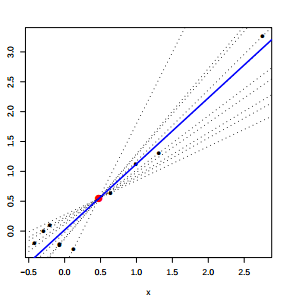
\includegraphics[scale=0.9]{img/rmc_atipico1.png}
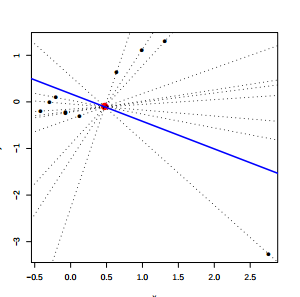
\includegraphics[scale=0.9]{img/rmc_atipico2.png}
\end{center}

\end{example}

\begin{example}[Sobre la distancia horizontal]

¿Y da igual lo atípico que sea un dato? La respuesta es que no. Si el dato es muy atípico en la variable respuesta ($Y$), pero es muy \textit{típico} en la variable regresora, la recta no se devía tanto. Vamos a verlo y después explicamos la razón.

Esta es la recta, en la que hemos ignorado los 3 datos que parecen ``atípicos''.
\begin{center}
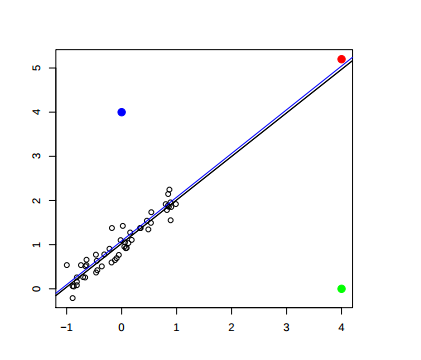
\includegraphics[scale=0.9]{img/sobredistanciahorizontal1.png}
\end{center}

Ahora calculamos las rectas teniendo en cuenta sólo uno de los puntos.

\begin{center}
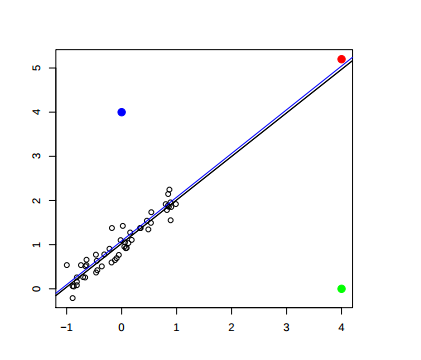
\includegraphics[scale=0.4]{img/sobredistanciahorizontal1.png}
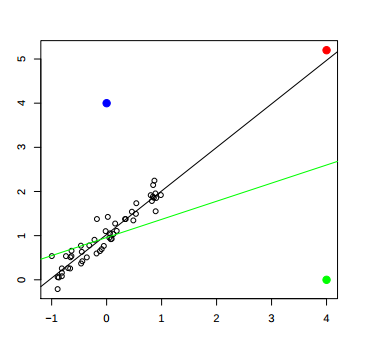
\includegraphics[scale=0.4]{img/sobredistanciahorizontal2.png}
\end{center}

Vemos que la recta azul no se desvía apenas de la original, mientras que la recta verde si se desvía un montón. ¿Esto a qué se debe? A que importa más la distancia horizontal de la media que la distancia vertical. Si vamos a la expresión de la recta de mínimos cuadrados como promedio de las pendientes \label{rmc::promediopendientes} vemos que hay un término $\frac{(x_i - \gor{x})}{S_{xx}}$ que hemos tomado como pesos para ponderar y en este caso, la distancia horizontal $(x_i - \gor{x})$ está multiplicando en el numerador.



\end{example}





\subsubsection{Introduciendo ``aleatoreidad'' para poder hacer IC}

Sea $\{ε_i\}$ siendo $ε_i \sim N(0,σ^2)$. Lo habitual es no saber cómo han sido generados los datos y es probable que no vayamos a conocer con exactitud absoluta la recta de mínimos cuadrados. Es por ello que suponemos el siguiente modelo para la variable respuesta:

\[
Y_i = β_1 x_i + β_0 + ε_i
\]


Tenemos que $\bar{y}_i \sim N$, ya que es una combinación lineal de variables normales \textbf{independientes} (como vimos en el Tema 1).


\begin{example}
Sea $σ=1, β_0 = 0 y β_1 = 1$.

Entonces el modelo es:

\[
Y_i = x_i + ε_i
\]

Fijamos $n=10$ y generamos las respuestas para $x_i = i$. Además, repetimos el experimento 6 veces y calculamos las rectas de mínimos cuadrados, obteniendo:

\begin{center}
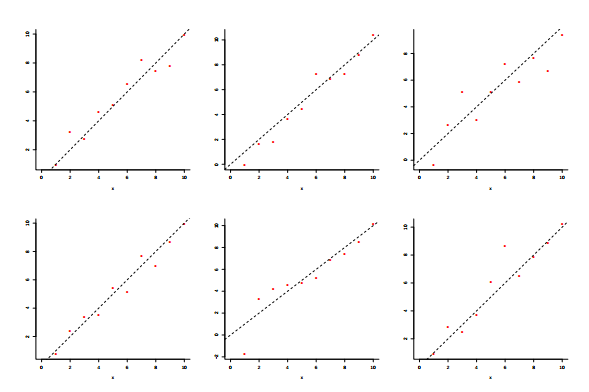
\includegraphics[scale=0.6]{img/6ejemplosRegresion.png}
\end{center}

Vemos que obviamente las rectas no son las mismas. Esto se debe al $ε_i$ introducido. ¿Cuáles son los valores que toman $β_1$ y $β_0$? Habiendo repetido el experimento 1000 veces, obtenemos los siguientes histogramas:

\begin{center}
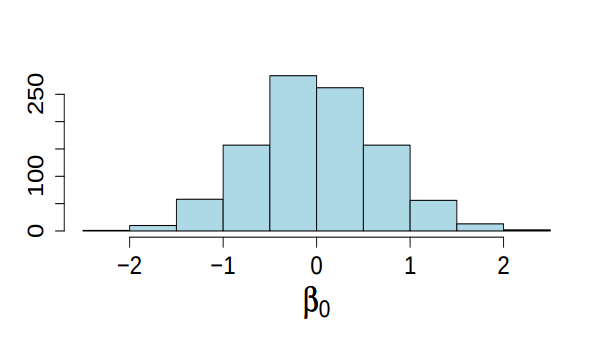
\includegraphics[scale=0.3]{img/1000vecesb0.png}
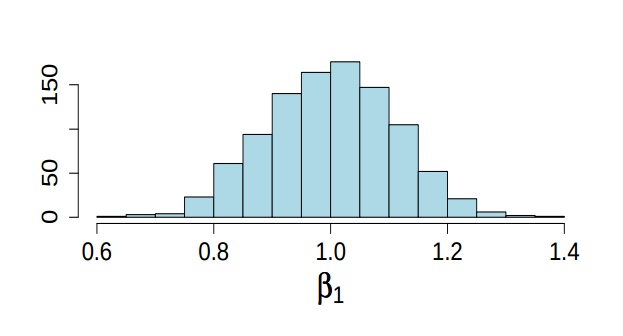
\includegraphics[scale=0.3]{img/1000vecesb1.png}
\end{center}

Vemos que no siempre es el mismo valor. Sabemos (por cómo hemos construido los datos) que $β_0 = 0$ y $β_1 = 1$, pero nuestra manera de calcularos (debido a $ε_i$) no siempre nos da el valor concreto.


\end{example}

El ejemplo anterior nos muestra que en realidad, estamos estimando $β_i$, aunque no nos guste y ahora tenemos que planternos ¿cómo de buenos son nuestros estimadores? Tal vez son una mierda, o tal vez son insesgados.

Para ello, vemos que al haber añadido un error $\epsilon_i \sim N(0,σ^2)$, tenemos:

\[
Y_i = β_0 + β_1x + ε_i \implies Y_i \equiv N(β_0 + β_1X_i, σ^2)
\]


\subsubsection{Estimando $β_1$}

\begin{prop}
Nuestro estimador ``pendiente de la recta de mínimos cuadrados:'' $\hat{β_1}$  cumple

\[
\hat{β_1} \equiv N\left(β_1,\frac{σ^2}{S_{xx}} \right)
\]

\end{prop}

\begin{proof}
Él en clase lo ha hecho al revés. Muchos cálculos para llegar a la conclusión, pero aquí molamos más. En algún momento \textcolor{red}{revisará} alguien los apuntes y completará.

\begin{itemize}
	\item $\esp{\hat{β_1}} = β_1$
	\item $\var{\hat{β_1}} = ... = \displaystyle\frac{σ^2}{S_{xx}}$
\end{itemize}
\end{proof}

\subsubsection{Estimando $β_0$}

\begin{prop}
Nuestro estimador ``término independiente de la recta de mínimos cuadrados:'' $\hat{β_0}$  cumple

\[
\hat{β_0} = N\left(β_0 , σ^2 \left( \frac{1}{n} + \frac{\gor{x}^2}{S_{xx}}\right)  \right)
\]
\end{prop}

\begin{proof}
\begin{itemize}
	\item $\esp{\hat{β_0}} = β_0$
	\item
	$\var{\hat{β_0}} = \var{\gor{Y}} + \var{\hat{β_1}\gor{X}} - 2 \cov{(\gor{Y},\hat{β_1}\gor{X}}$

 	\subitem Calculamos: $\cov{(\gor{Y},\hat{β_1}\gor{X}}$ utilizando cosas del tema 1

 	\[
		\cov{(\gor{Y},\hat{β_1}\gor{X}} = \cov{(\frac{1'_n \gor{Y}}{n},α\gor{Y}} = \frac{1}{n}1'_nσ^2
 	\]
 	debido a que $α = 0$.

 	Ademas de ser incorrelados, son \textbf{independientes}. ¿Porqué? Porque conjutamente son normales, es decir \[
 		\begin{pmatrix} \gor{Y} \\ \hat{β_1} \end{pmatrix} \equiv A\gor{Y} \equiv N_2
 	\]
\end{itemize}

\end{proof}


\textbf{Conclusiones:}
\begin{align*}
\gor{Y} &\text{ es indepediente de } \hat{β_1}\\
\hat{β_1} &\equiv \left(β_1,\frac{σ^2}{S_{xx}}\right)\\
\hat{β_0} &\equiv \left(β_0,σ^2 \left( \frac{1}{n} + \frac{\vec{x}^2}{S_{xx}}\right)\right)
\end{align*}

¿Son estas las variables $\hat{β_1} $ y $\hat{β_2}$ normales una normal conjunta? No, \textbf{no son una normal conjunta} ya que no son independientes. Intuitivamente es fácil de ver. En una recta, si aumentamos la pendiente (y estamos en el primer cuadrante) entonces el término independiente disminuye. Esta dependencia tiene que aparecer. Vamos a estudiar la covarianza entre los estimadores:

\[
\cov{(β_1,β_2} = \cov{(\gor{Y} - \hat{β_1}\gor{x}, \hat{β_0}} = ... = -\gor{x}\frac{σ^2}{S_{xx}}
\]



\subsubsection{IC y Contrastes para $β_1$}

Recordamos que \[ \hat{β}_1 \equiv N\left(β_1,\frac{σ^2}{S_{xx}}\right)\]

Podemos normalizar y buscar una catidad pivotal (como hacíamos en estadística I)

\[
\frac{\hat{β_1} - β_1}{\frac{σ}{S_{xx}}} \equiv N\left(0,1\right)
\]

Pero aquí nos encontramos con que necesitamos $σ$, la varianza de los errores. Esta varianza a menudo no es conocida (porque no sabemos con exactitud cuál es la recta verdadera) y tenemos que estimarla.

Para estimarla, parece razonable usar \[ \hat{σ} = S_R =\frac{\sum_{i=1}^n e_i^2}{n-2}\]

\begin{expla}
Recordamos que para que estimar la varinza, utilizamos (por el lema de fisher) $n-1$ de denominador para que el estimador sea insesgado. Esto sale de que en la demostración, hay una matriz de rango $n-1$ ya que existe una restricción.

Siguiendo este razonamiento, en este caso tenemos 2 restricciones\footnote{$\sum e_i = 0$ y $\sum e_ix_i = 0$}, por lo que si lo demostráramos rigurosamente, aparecería una matriz de rango $n-2$ y por eso es el denomiador. De esta manera, conseguimos un estimador insesgado.

\end{expla}

Además, $S_R$ se denomina \concept{varianza residual}

\begin{prop}
Una pequeña generalización del lema de Fisher:
\[
\frac{(n-2)S_{R}^2}{σ^2} \equiv \chi_{n-2}^2
\]

Además, es independiente de $\hat{β_1}$

\end{prop}



\begin{proof}
Esta proposición es un caso particular de un teorema que veremos más adelante.
\end{proof}


Ahora que ya tenemos estimada la varianza, podemos calcular:


\[
\frac{\hat{β_1}-β_1}{\frac{S_R}{\sqrt{S_{xx}}}} = \frac{\hat{β_1}-β_1}{\displaystyle\frac{\frac{σ}{\sqrt{S_{xx}}}}{\frac{S_R}{σ}}}
\]

En el numerador tenemos una $N(0,1)$ y en denominador una $\chi^2$ dividida por sus grados de libertad. Esto es por definición de $\mathcal{T}$ \footnote{T de Student} es una $\mathcal{T}$ (T-Student) con $n-2$ grados de libertad.

\begin{prop}
Ahora que conocemos la distribución, podemos calcular el intervalo de confianza  para la pendiente de la recta.

\textcolor{red}{No entiendo nada de esto.}
\[
IC_{1-α}(β_1) \equiv \left[ \hat{β_1} \pm \mathcal{T}_{n-2,\frac{α}{2}}\frac{S_R}{\sqrt{S_{xx}}}\right] \equiv \left[ \gor{Y} \pm \mathcal{T}_{n-1,\frac{α}{2}}\frac{S_R}{\sqrt{n}} \right]
\]
\end{prop}

\subsubsection{Contraste en R}


\begin{lstlisting}
> # Ajusta el modelo
> regresion = lm(Fracaso~Renta)
> summary(regresion)

> lm(formula = Fracaso ~ Renta)
Residuals:	Min	1Q	Median	3Q	Max
		-7.8717 -3.7421	0.5878	3.0368	11.5423
---
Coefficients:	Estimate Std.	Error 	t-value	Pr(>|t|)
(Intercept)	38.4944		3.6445	10.562	7.37e-10 ***
Renta 		-1.3467		0.2659	-5.065	5.14e-05 ***
---
Signif. codes: [...]
Residual standard error: 4.757 on 21 degrees of freedom
Multiple R-Squared: 0.5499,
Adjusted R-squared: 0.528
\end{lstlisting}


Aquí, la fila de intercept es el término independiente y renta es la pendiente. Además, los p-valores son para el contraste $\hat{β_i} = 0$, dentro de la hipótesis $β_i \geq 0$. \footnote{Si queremos contrastar si es positivo, nos vamos al caso límite que lo separa y contrastamos eso}.

En este caso, el p-valor para $\hat{β_1} = 7.37e-10$, con lo que no podemos rechazar la hipótesis.


\subsubsection{Predicciones}

Sea $(x_1,y_1),...,(x_n,y_n) \to y_i = β_0 + β_1x_i + ε_i$.

Dado una nueva observación $x_0$, tenemos 2 problemas para predecir:

\begin{itemize}
	\item \textbf{Inferencia sobre $m_0 \equiv \esp{y_0 | x_0} = β_0 + β_1x_0$}

	En este caso, $$\hat{m_0} = \hat{β_0} + \hat{β_1}x_0$$

	¿Cómo es este estimador?

	\[\esp{\hat{m_0}} = β_0 + β_1x_0 = m_0\]
	\[\var{\hat{m_0}} = ... = σ^2\left[\frac{1}{n} + \frac{(x_0-\bar{x})^2}{S_{xx}} \right] \]

	\subitem Intuitivamente, lo que significa el segundo sumando de la varianza es que ``cuanto más cerca esté $x_0$ de la media, mejor será la estimación''.

	\textbf{Conclusión:}

	\[
		\hat{m_0} \sim N\left( m_0, σ^2\left[\frac{1}{n} + \frac{(x_0-\bar{x})^2}{S_{xx}} \right]\right)
	\]



	\subitem \textbf{Intervalo de confianza} para $m_0$ utilizando la fórmula de intervalos de confianza:

	\[
IC_{1-α}(m_0) \equiv \left[ \hat{m_0} \pm \mathcal{T}_{n-2,\frac{α}{2}}S_R\sqrt{\frac{1}{n} + \frac{(x - \gor{x})^2}{S_{xx}}}\right]
\]

	\item \textbf{Predecir $Y_0$} usamos de nuevo:

	\[
\hat{Y_0} = \hat{β_0} + \hat{β_1}x \to Y_0 - Y \equiv N\left( 0, σ^2\left( 1 + \frac{1}{n}+  \frac{(x-\gor{x})^2}{S_{xx}}\right) \right)
	\]

	Donde la varianza ha sido calculada:

	\[
	\var{Y_0 - \hat{Y_0}} = \underbrace{\var{Y_0}}_{σ^2} - \var{\hat{Y_0}} + \underbrace{2 \cov{Y_0,\hat{Y_0}}}_{ = 0 \text{ (indep.) }} = σ^2 + σ^2\left( \frac{1}{n}+  \frac{(x-\gor{x})^2}{S_{xx}} \right)
	\]


	Este es un problema más complicado, ya que tenemos que tener en cuenta el término de error $ε_i$ y es por esto que aparece el 1 en la varianza. Tenemos que tener en cuenta la incertidumbre.

	Estandarizando y cambiando $σ$ por $S$, tenemos:

	\[
	\frac{Y_0 - \hat{Y_0}}{S_r \sqrt{1 + \frac{1}{n} + \frac{(x-\gor{x})^2}{S_{xx}}}} \equiv \mathcal{T}_{n-2}
	\]

	Ya que tenemos una normal estandarizada dividida por su .... que por definición, es una $\mathcal{T}$ de student.

	Ahora, vamos a construir el \concept{intervalo de predicción} (cambia ligeramente la interpretación)

	\[
1 - α = P\left\{ -\mathcal{T}_{n-2;\frac{α}{2}} < \frac{Y_0 - \hat{Y_0}}{...} < \mathcal{T}_{n-2;\frac{α}{2}}    \right\} = P \left\{ Y_0 \in \left[ \hat{Y_0} \pm \mathcal{T}_{n-2;\frac{α}{2}} S_R \sqrt{1+\frac{1}{n}+...} \right]  \right\}
	\]
\end{itemize}

Ahora vamos a hacer unos ejemplos numéricos.

\begin{example}Seguimos con el ejemplo de la renta.

\begin{center}
\begin{tabular}{c|c|c}
&media&desviación típica\\\hline
\% fracaso & 20.73 & 6.927\\
renta &13.19 $·10^{3}$ & 3.814
\end{tabular}
\end{center}

\setcounter{part}{0}
\ppart IC para $β_1$ de nivel $95\%$.
\ppart IC para \% de fracaso medio si la renta es de $14.000$ euros.

\spart

\[
-1.3467 \pm \mathcal{T}_{21;0.025} · (0.2659)
\]

Donde el $-1.3467$ es el estimador $\gor{m_0}$ que obtenemos de la salida de $R$. Lo mismo el $0.2659$, que es el error típico.

\spart
\[ \gor{Y_0} = 38.49 - (0.3467) · \underbrace{14}_{x_0} = 19.64\%\]

Siendo este el estimador, vamos a construir el intervalo de confianza. \footnote{Podría ser que nos pidieran el intervalo de predicción, pero en ese caso estarían pidiendo el intervalo de ...... para predecir.}

\[
IC = 19.64 \pm (2.06)(4.757)\sqrt{\frac{1}{23}+\frac{(14-13.19)^2}{S_{xx}}}
\]
Donde $S_{xx} = 320.06$ y podemos calcularlo despejando de cualquiera de las fórmulas:

\[
E.T.(\gor{β_1}) = \frac{S_R^2}{S_{xx}}
\]
\[
6. = \frac{S_{xx}}{n-1}
\]

\end{example}


\obs Todos estos cálculos y todas estas fórmulas se basan en muchas hipótesis (como que la distribución del error sigue una distribución normal). Pero podría ser que esto no ocurriera y estuviéramos suponiendo un modelo falso. Para ello, en estadística existe el \concept{Diagnóstico del modelo}. Este diagnóstico, consiste en comprobar si las hipótesis del modelo son \textbf{aceptables} para los datos disponibles. ¡Ojo! Aceptable... Puede haber muchos modelos aceptables para un mismo conjunto de datos.

Este diagnóstico se suele basar en el análisis de los residuos del modelo.

\begin{example}
	Vamos a ver a ojo unos cuantos ejemplos. Vamos a utilizar que $cor{e,\gor{y}} = 0$ bajo el modelo (como calculamos anteriormente)

\begin{center}
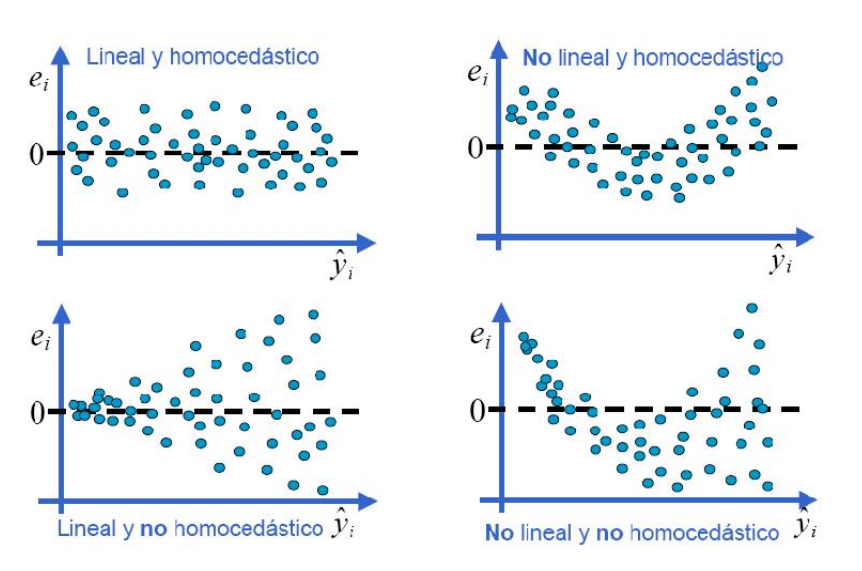
\includegraphics[scale=0.6]{img/diagmodelo.png}
\end{center}

De estos 4 gráficos, el bueno es el primero, ya que los demás no complen alguno.
\end{example}

\begin{example}
Vamos a ver otro ejemplo, donde arriba están los datos y abajo los residuos. Mirando sólo la fila de arriba podríamos saber si nuestro modelo para la regresión se cumple o sino.


\begin{center}
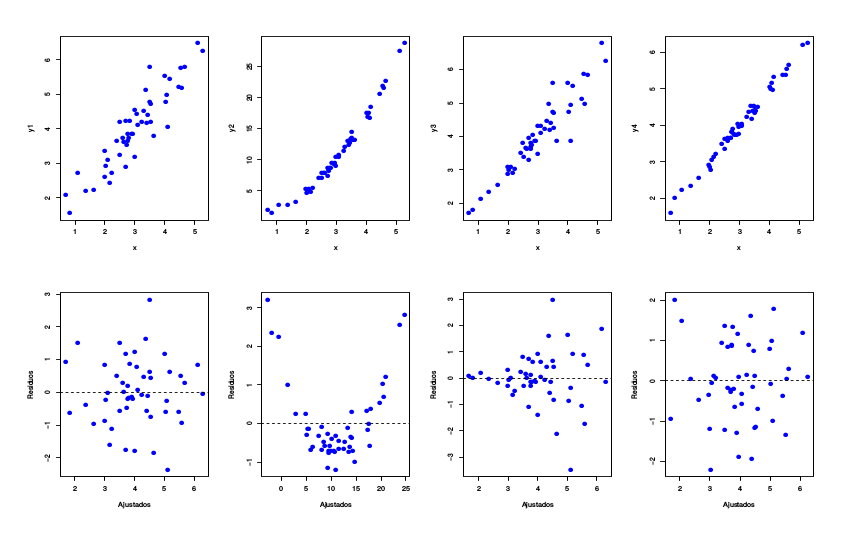
\includegraphics[scale=0.6]{img/diagmodelo_2.png}
\end{center}

Vemos que el primero y el último si tienen este modelo como aceptable, ya que en los residuos no hay ningún patrón (y se cumple que la correlación es 0).

En el segundo, podríammos suponer que es bueno, pero al diagnosticar el modelo mirando los residuos, vemos que no. El diagnóstico del model \textbf{magnifica los errores}.

En el cuarto, vemos más claro que es heterocedástico y que no se cumple el modelo supuesto.
\end{example}

En regresión múltiple veremos que no podemos ver los datos, ya que son demasiadas variables, pero sí podemos estudiar los residuos como acabamos de hacer en los ejemplos anteriores.

\subsection{Regresión lineal múltiple}

El ejemplo que vamos a estudiar en regresión múltiple es el consumo de gasolina en EEUU intentando predecirlo a partir de unas cuantas variables. Las variables regresoras son:

\begin{center}
\begin{tabular}{cccccccc}
State&Drivers&FuelC&Income&Miles&MPC&Pop&Tax\\\hline
AL&3559897&2382507&23471&94440&12737.00&3451586&18.0\\
AK&472211&235400&30064&13628&7639.16&457728&8.0\\
AZ&3550367&2428430&25578&55245&9411.55&3907526&18.0
\end{tabular}
\end{center}

\subsubsection{Notación}


\begin{itemize}
	\item $n$ es el número de observaciones, en este caso, el número de estados.
	\item $k$ es el número de atributos.
	\item $ε_i \sim N(0,σ^2)$
	\item $n\geq k+2$: esta hípótesis  es muy necesaria.\footnote{En la estadística, habría que rehacer el modelo para cuando $k>n$. ¿Y cuándo $k>n$? ¿Cuándo puede ocurrir esto? Cada vez más hay más información para cada individuo. En estudios genéticos por ejemplo, que hay millones de genes pero no se pueden hacer el estudio con millones de personas... \textbf{LA MALDICIÓN DE LA DIMENSIONALIDAD} que decimos en Introducción previa a los Fundamentos Básicos del Aprendizaje Automático.\\ Una posible solución al problema es un algoritmo que filtre los atributos que son importantes.}
\end{itemize}

Regresión simple es un caso particular de múltiple, tomando $k=1$.

\subsubsection{Modelo}

El modelo es:

\textcolor{red}{Completar de las traspas}

Podemos agruparlo en forma matricial:

\textcolor{red}{Completar de las traspas}

\paragraph{Recordamos} que en el tema 1 vimos unas cuantas formas cuadráticas útiles para normales multivariantes con matriz de variazas $σ^2I_n$ y media arbitraria.

\textcolor{red}{Completar de las traspas}

¿Cómo estimarías $β$ a partir de $Y$ y $X$?

Podemos hacer la proyección de $Y$ sobre $\mathcal{V}$

Con esto, parece razonable estimar $µ$ mediante la proyección ortogonal de $T$ sobre $\mathcal{V}$ para obtener $\gor{Y} = X\gor{β}$. Equivalentemente: $||Y-X\gor{β}||^2 \leq || Y-Xβ||^2, ∀β\in ℝ^{k+1}$


\textcolor{red}{completar cosas que faltan}

\paragraph{Resumen}
Si
\[ Y \equiv N_n (Xβ,σ^2I_n)\]

entonces, la proyección sobre \_\_\_\_\_\_\_ es:
\[
\hat{Y} = X\hat{β} = HY
\]
donde $H = X(X'X)^{-1}X^{-1}$. Además, \[\hat{β} = (X'X)^{-1}X'Y\]


Esto tiene como consecuencia que el vector de residuos es: $e = Y-\hat{Y} = (I-H) Y$

En cuanto a la interpretación geométrica, los residuos es la recta vertical que une la proyección ($\hat{Y}$) con el vector real ($Y$).

\subsubsection{Distribución de $\hat{β}$}
\[
β \equiv N_{k+1}\left(β,σ^2(X'X)^{-1}\right)
\]

Y la regresión simple, es un caso particular de esta fórmula.

\paragraph{Consecuencias:}

\begin{itemize}
	\item ¿Cuál es la distribución marginal de $\hat{β_j}$ a partir de la que hemos visto de la conjunta? Como vimos en el tema 1, es también una normal, con el correspondiente valor del vector $β$ como media y el elemento $j,j$ de la diagonal.
	\[ β_j \equiv N\left(β_j, σ^2q_{jj}\right)\]

	Ahora, podemos estandarizar:

	\[
	\frac{\hat{β_j}-β_j}{σ\sqrt{q_{jj}}} \equiv N(0,1)
	\]

	Y utilizando que $S_R$ es independiente de $σ$ y la definición de $t-$student tenemos:

	\[
	\frac{\hat{β_j}-β_j}{S_R\sqrt{q_{jj}}} \equiv \mathcal{T}_{n-k-1}
	\]

	¿Cuál es el intervalo de confianza?

	\[
		IC_{n-α}(β_j) \equiv \left[\hat{β_j}\pm \mathcal{T}_{n-k-1}\underbrace{S_R\sqrt{q_{jj}}}_{\text{Error típico de }β_j} \right]
	\]

	Y, como en regresión simple, estudiamos $H_0 : β_j = 0$:
	\[
		R = \left\{ \frac{|β_j|}{S_R\sqrt{q_{jj}}} > \mathcal{T}_{n-k-1;\frac{α}{2}} \right\}
	\]
\end{itemize}

En las traspas encontramos una salida de regresión múltiple de $R$. La columna estimate es el vector $\hat{β}$, el p-valor

\appendix
\chapter{Ejercicios}
% -*- root: ../EstadisticaII.tex -*-

%%%%%%%%%%%%%%%%%%%%%%%%%%%%%%%%%%%%%%%%%%%%%%%%%%%%%%%%%%%%%%%%%%%%%%%%%%%%%%%%%%%%%%%%%%%%%%%
%%% 																						%%%
%%% 								HOJA 	1												%%%
%%% 																						%%%
%%%%%%%%%%%%%%%%%%%%%%%%%%%%%%%%%%%%%%%%%%%%%%%%%%%%%%%%%%%%%%%%%%%%%%%%%%%%%%%%%%%%%%%%%%%%%%%

\section{Hoja 1}

\begin{problem}[1]
Sea $\vec{Y} = (Y_1,Y_2,Y_3)' ≡ N_3(\vec{µ},Σ)$, donde \[\vec{µ} = (0,0,0)'\;
Σ =\begin{pmatrix}
1&0&0\\
0&2&−1\\
0&−1&2
\end{pmatrix}
\]


\ppart  Calcula la distribución del vector $\vec{X} = (X_1,X_2)$, donde $X_1 = Y_1 + Y_3$ y $X_2 = Y_2 + Y_3$.
\ppart ¿Existe alguna combinación lineal de las variables aleatorias $Y_i$ que sea independiente de $X_1$?

\solution
\doneby{Dejuan}


\spart 
\[
\begin{pmatrix}X_1 \\ X_2 \end{pmatrix} = \begin{pmatrix} Y_1 + Y_3 \\ Y_2 + Y_3 \end{pmatrix} = \begin{pmatrix} 1&0&1\\0&1&1 \end{pmatrix} \begin{pmatrix} Y_1\\Y_2\\Y_3 \end{pmatrix} 
\]

Ya tenemos la matriz $A$ que cumple $\vec{X} = A \vec{Y}$. Utilizando las propiedades de esperanza y varianza (\ref{propiedades:esperanzaYvarianza}):

\[\esp{\vec{X}} = \esp{A\vec{Y}} = A\esp{\vec{Y}} = \begin{pmatrix} 1&0&1\\0&1&1 \end{pmatrix} \begin{pmatrix} 0 \\0\\0\end{pmatrix} = \begin{pmatrix} 0 \\0\\0\end{pmatrix}\]

\[\var{\vec{X}} = \esp{A\vec{Y}} = AΣA' = \begin{pmatrix} 1&0&1\\0&1&1 \end{pmatrix} \begin{pmatrix}
1&0&0\\
0&2&−1\\
0&−1&2
\end{pmatrix} \begin{pmatrix} 1&0\\0&1\\1&1 \end{pmatrix} = \begin{pmatrix}3&1\\1&2\end{pmatrix}\]

\paragraph{Conclusión:}

\[\begin{pmatrix}X_1 \\ X_2 \end{pmatrix} \equiv N_1\left( \begin{pmatrix}0\\0 \end{pmatrix},\begin{pmatrix}3&1\\1&2\end{pmatrix} \right)\]


\spart Llamos $Z = a_1 Y_1 + a_2Y_2+a_3Y_3$.


Estas variables serán independientes si se distribuyen conjuntamente como una normal multidimensional y si $\cov{Z,X_1} = 0$.


Vamos a ver la covarianza. Utilizando la propiedad definida en \ref{propiedad:CovCombinacionLineal}, tenemos que

\[
\cov{a_1Y_1 + a_2Y_2 + a_3Y_3 , X_1} = \cov{A\vec{Y},B\vec{Y}}
\]

Siendo $A = (a_1,a_2,a_3)$ y $B=(1,0,1)$

Entonces \[\cov{A\vec{Y},B{\vec{Y}}} = (a_1,a_2,a_3) \begin{pmatrix} 1&0&0\\0&2&-1\\0&-1&2\end{pmatrix} \begin{pmatrix} 1\\0\\1 \end{pmatrix}\]

Operando obtenemos $\cov{A\vec{Y},X_1} = a_1 - a_2 + 2a_3$.



Ahora sólo hace falta ver que se distribuyen conjuntamente como una normal bivariante. Esto lo tenemos asegurado, pues ``\textit{El vector se distribuye normalmente porque lo podemos escribir en la forma AY, para una matriz A.}''\footnote{Cito textualmente de un correo envíado por José Ramón, profesor de la asignatura}
\end{problem}


\begin{problem}[2]

Sea $\vec{X} = (X_1 , X_2 , X_3 )$ un vector aleatorio con distribución normal tridimensional con vector de medias $\vec{µ} = (0, 0, 0)$ y matriz de covarianzas
\[ Σ = \begin{pmatrix}
4&0&−1 \\
0&5&0\\
−1&0&2
\end{pmatrix}
\]

\ppart Determina razonadamente cuáles de los siguientes pares de variables o vectores aleatorios son independientes y cuáles no:  

\textbf{(i)}: $X_1$ y $X_2$

\textbf{(ii)}: $(X_1 , X_3 )$ y $X_2$ 

\textbf{(iii)}: $X_1$ y $X_1 + 3X_2 − 2X_3$

\ppart Determina una matriz B tal que la variable aleatoria $(X_2 , X_3 )B(X_2 , X_3)'$ tenga distribución $χ^2_2$.

\solution

\spart 

\textbf{(i)} $X_1$ y $X_2$ son independientes porque son marginales de una distribución multivariante conjunta y tienen covarianza 0 (elemento $a_{12}$ de la matriz)

\textbf{(ii)} $X_1$ y $X_2$ son independientes porque son marginales de una distribución multivariante conjunta y tienen de matriz de covarianzas el vector idénticamente nulo. Vamos a verlo, aunque para ello construimos $\vec{Z} = (X_1,X_3,X_2)$, cuya matriz de covarianzas es:\[ Σ_z = \begin{pmatrix}
4&-1&0\\
-1&5&0\\
0&0&2
\end{pmatrix}\]
Entonces $\cov{(X_1,X_3)',X_2} = \begin{pmatrix}\cov{X_1,X_2} \\ \cov{X_3,X_2}\end{pmatrix} = \begin{pmatrix}0\\0\end{pmatrix}$

\textbf{(iii)} $X_1$ y $X_1 + 3X_2 − 2X_3$. Utilizamos: $\cov{X_1 + 3X_2 − 2X_3,X_1} = \cov{A\vec{X},B\vec{X}} = AΣB' = BΣA'$
\[
\cov{X_1 + 3X_2 − 2X_3,X_1} =
(1,3,-2) \begin{pmatrix}
4&0&−1 \\
0&5&0\\
−1&0&2
\end{pmatrix} \begin{pmatrix}1\\0\\0\end{pmatrix} = ... = 6
\]

Como la covarianza no es cero, entonces existe una relación lineal entre las variables y por ello no son independientes.

\spart 

Una $\chi^2_k$ es la distribución que tiene la suma de variables normales estandarizadas al cuadrado. Los $k$ grados de libertad corresponden a la cantidad de variables normales que sumamos.

Vemos que si tomamos $B=I$, obtenemos:

\[(X_2,X_3) \begin{pmatrix} 1&0\\0&1 \end{pmatrix} \begin{pmatrix}X_2\\X_3\end{pmatrix} = X_2^2 + X_3^2\]

Ya tenemos la suma los cuadrados de normales. Ahora sólo falta que estén estandarizadas, es decir que $X_i \sim N(0,1)$.

Ya están centradas en 0, con lo que sólo falta dividir por la varianza, es decir:

\[(X_2,X_3) \begin{pmatrix} \frac{1}{5}&0\\0&\frac{1}{2} \end{pmatrix} \begin{pmatrix}X_2\\X_3\end{pmatrix} = \frac{1}{5}X_2^2 + \frac{1}{2}X_3^2 = Z_2^2 + Z_3^2\]

donde 
\[Z_2 = \frac{1}{5}X_2^2 = \left(\frac{X_2}{\sqrt{5}}\right)^2 \to Z_2 \sim N(0,1)\]
\[Z_3 = \frac{1}{2}X_2^2 = \left(\frac{X_2}{\sqrt{2}}\right)^2 \to Z_3 \sim N(0,1)\]


\end{problem}
\begin{problem}[3]
Sea $(X, Y )$ un vector aleatorio con distribución normal bidimensional. Tanto $X$ como $Y$ tienen
distribución normal estándar. La covarianza entre $X$ e $Y$ es $ρ$, donde $|ρ| < 1$.

\ppart Determina cuál es la distribución del vector $(2X − 3Y , X + Y ) $.
\ppart Determina cuál es la distribución de la variable $(X^2 − 2ρXY + Y^2 )/(1 − ρ^2 )$.

\solution

\doneby{Dejuan}

\spart 
Llamamos 
\[
C = \begin{pmatrix} 2&-3\\1&1 \end{pmatrix}\begin{pmatrix}X\\Y\end{pmatrix}
\]

Tenemos que calcular $\esp{C},\var{C}$. Para ello, utilizamos las fórmulas de siempre

\[
\esp{C} = \esp{A\begin{pmatrix}X\\Y\end{pmatrix}} = A\esp{(X,Y)'} = A(0,0)' = \begin{pmatrix}0\\0\end{pmatrix}
\]
\[
\var{C} = \var{C(X,Y)'} = CΣC' = \begin{pmatrix} 2&-3\\1&1 \end{pmatrix} \begin{pmatrix} 1&\rho\\\rho &1\end{pmatrix}\begin{pmatrix} 2&1\\-3&1 \end{pmatrix} 
\]

La distribución del vector $(X,Y) \sim N_2\left(\esp{C},\var{C}\right)$


\spart 

Sea \[Z = \frac{Z_n}{Z_d} = \frac{(X^2 − 2ρXY + Y^2 )}{(1 − ρ^2 )}\]

Vemos que \[ Z_n = (X,Y)\begin{pmatrix} a&b\\c&d \end{pmatrix}\begin{pmatrix} X\\Y \end{pmatrix} = aX^2 + cXY+bXY+dY^2\implies \left\{ \begin{array}{c} a=d=1\\c+b=-2\rho \to c=b=-\rho \end{array}\right.\]

Ahora, dividimos todo por $Z_d$. ¿Qué hemos obtenido?

\[
\frac{1}{1-\rho^2}\begin{pmatrix}1&-\rho\\-\rho&1\end{pmatrix}
\]


Casualmente, esta matriz es la inversa de $Σ$

\[
\begin{pmatrix}1&\rho\\\rho&1\end{pmatrix}\frac{1}{1-\rho^2}\begin{pmatrix}1&-\rho\\-\rho&1\end{pmatrix} = \begin{pmatrix}1&0\\0&1\end{pmatrix}
\]

Con lo que \[Z = (X,Y)Σ^{-1}(X,Y)' = (X-0,Y-0)Σ^{-1}(X-0,Y-0)' \sim \chi^2_2\]

\end{problem}

\begin{problem}[4]
\label{ejrc:4-hoja1}
Sean $Y_1$ e $Y_2$ dos variable aleatorias independientes con distribución normal estándar.

\ppart  Demuestra que el vector $\vec{Y} = (Y_1 , Y_2 )$ tiene distribución normal bidimensional y calcula la distribución del vector $\vec{X} = (2Y_1 + Y_2 , Y_2 − 2Y_1 )$.

\ppart  ¿Son las dos distribuciones marginales de X independientes? Determina una matriz B tal que $X'BX$ tenga distribución $χ^2$ con 2 grados de libertad.
\solution

\doneby{Dejuan}

\spart
\doneby{Jorge}

Tomemos la función característica del vector aleatorio que tiene ambas v.a. $Y=(Y_1,Y_2)$:

\[φ_Y(t) = \mathbb{E}(e^{it'Y}) = \mathbb{E}(e^{it_1Y_1+it_2Y_2})=\]

Puesto que $Y_1,Y_2$ son independientes:

\[= \mathbb{E}(e^{it_1Y_1})·\mathbb{E}(e^{it_2Y_2}) = φ_{Y_1}(t_1)·φ_{Y_2}(t_2) = e^{-\frac{t_1^2}{2}}·e^{-\frac{t_2^2}{2}}= e^{-\frac{t_1^2+t_2^2}{2}}\]

Que coincide con la función característica de una normal bidimensional $Y\sim N_2(0,I)$.

El vector de $n$ normales independientes se distribuye normalmente. En este caso, como $Y_1,Y_2$ son normales independientes, $(Y_1,Y_2) \sim N(µ,Σ)$, donde:

\[µ = \begin{pmatrix}0\\0\end{pmatrix}\;\;\; Σ = \begin{pmatrix}1&0\\0&1\end{pmatrix}\]

\[\vec{X} = (2Y_1 + Y_2 , Y_2 − 2Y_1 ) \to \begin{pmatrix}X_1\\X_2\end{pmatrix} = \begin{pmatrix}2&1\\1&-2\end{pmatrix}\begin{pmatrix}Y_1\\Y_2\end{pmatrix}\]

Entonces, vamos a calcular la distribución de $\vec{X}$

\[
\esp{\vec{X}} = \esp{A\vec{Y}} = A\esp{Y} = \begin{pmatrix}0\\0\end{pmatrix}
\]
\[
\var{\vec{X}} = \var{A\vec{Y}} = A\var{\vec{Y}}A' = AA' = AA = \begin{pmatrix} 5&0\\0&5\end{pmatrix}
\]

\spart $X_i \sim N(0,5)$. Además, $\corr{X_1,X_2} = 0$.

Sí son independientes porque vienen de un vector normal y son incorreladas.


\textbf{$\chi^2$:} Una $\chi^2_k$ es una suma de $k$ normales estandarizadas, asique si tomamos $B = Σ^{-1} = \begin{pmatrix}1/5&0\\0&1/5\end{pmatrix}$ tendremos normales al cuadrado estandarizadas.

\[
(X_1,X_2)\begin{pmatrix}1/5&0\\0&1/5\end{pmatrix}\begin{pmatrix}X_1\\X_2\end{pmatrix} = \frac{1}{5}X_1^2 + \frac{1}{5}X_2^2 = Z\sim \chi^2_2
\]



\end{problem}

\begin{problem}[5]

Sea $(X, Y )$ un vector aleatorio con función de densidad

\[
f (x, y) = \frac{1}{2π}\exp\left[\frac{1}{2}\left(x^2 − 2xy + 2y^2\right)\right]
\]

\ppart Calcula la distribución condicionada de $X$ dado $Y = y$, y la de $Y$ dado $X = x$.

\solution

Mirando la función de densidad y comparándola con la de la normal, podemos escribir:
\[
\begin{pmatrix}X\\Y \end{pmatrix} \equiv N_2\left(\begin{pmatrix}0\\0\end{pmatrix},\begin{pmatrix}1&-1\\-1&2\end{pmatrix}^{-1}\right)
\]

Aplicando las fórmulas vistas en teoría \ref{form::EspVarCondicionada}

\[
E(X|Y=y) = μ_y + Σ_{21}Σ_{11}^{-1}(X-μ_x) = 0 + \frac{1}{1}(y-0) = y
\]
\[
E(Y|X=x) = μ_x + Σ_{21}Σ_{11}^{-1}(Y-μ_y) = 0 + \frac{1}{2}(x-0) = \frac{x}{2}
\]

\end{problem}

\begin{problem}[6]
Sea $\vec{X} = (X_1 , X_2 )$ un vector aleatorio con distribución normal bidimensional con vector de medias $(1, 1)$ y matriz de covarianzas
\[Σ = \begin{pmatrix} 3&1\\1&2\end{pmatrix}\]

Calcula la distribución de $X_1 + X_2$ condicionada por el valor de $X_1 − X_2$ .
\solution

\[\begin{pmatrix}Z_1\\Z_2\end{pmatrix} = \begin{pmatrix}1&1\\1&-1\end{pmatrix}\begin{pmatrix}X_1\\X_2\end{pmatrix}\]

Entonces, calculando como siempre obtenemos:

\[
\begin{pmatrix}Z_1\\Z_2\end{pmatrix} \equiv N_2 \left(\begin{pmatrix}2\\0\end{pmatrix},\begin{pmatrix}7&1\\1&3\end{pmatrix}\right)
\]

Sabemos que la distribución va a ser normal, por lo que necesitamos $\esp{Z_1 | Z_2}$ y $\var{Z_1 | Z_2}$


Utilizando las fórmulas tenemos:

\[
\esp{Z_1|Z_2} = µ_1 + Σ_{12}Σ_{22}^{-1}(Z_2 - µ_2) = 2 + 1 \frac{1}{3}(Z_2 - 0) = \frac{7}{3}Z_2
\]

\[
\var{Z_1|Z_2} = Σ_{11} - Σ_{12}Σ_{22}^{-1}Σ_{21} = 7 - 1\frac{1}{3}1 = \frac{20}{3}
\]

Entonces, \[
(Z_2 | Z_1) = (X_1+X_2 | X_1 - X_2) \sim N_2\left( \frac{7}{3}(X_1 - X_2), \frac{20}{3} \right)
\]


\end{problem}

\begin{problem}[7]
Sea $X = (X1,X2,X3)'$ un vector aleatorio con distribución normal tridimensional con vector de medias $(0,0,0)'$ y matriz de covarianzas
\[
Σ =
\begin{pmatrix}
1&2&−1\\
2&6&0\\
−1&0&4
\end{pmatrix}
\]


Definamos las v.a. $Y_1 = X_1 + X_3, Y_2 = 2X_1 − X_2 $ e $ Y_3 = 2X_3 − X_2$. Calcula la distribución de $Y_3$ dado que $Y_1=0$ e $Y_2=1$.

\solution


Lo primero es descubrir la matriz de la combinación lineal y calcular la distribución, esto es:
\[
\begin{pmatrix} Y_1\\Y_2\\Y_3\end{pmatrix} = \begin{pmatrix}1&0&1\\2&-1&0\\0&-1&2\end{pmatrix}\begin{pmatrix}X_1\\X_2\\X_3\end{pmatrix} \equiv N_3 \left( \begin{pmatrix}0\\0\\0\end{pmatrix}, \begin{pmatrix}3&-2&4\\-2&2&-2\\4&-2&22 \end{pmatrix} \right)
 \]



Ahora vamos a calcular las condicionadas.  Sabemos que $Y_3 | Y_1=0, Y_2=1 \sim N_1 (µ_{2.1},Σ_{2.1})$. 

Hacemos la división:

\[
Σ = \left(\begin{array}{c|c}Σ_{11} & Σ_{12}\\\hlineΣ_{21} & Σ_{22}\end{array}\right) = \left(\begin{array}{cc|c} 3 & -2 & 4\\-2&2&-2\\\hline 4&-2&22\end{array}\right)
\]

\[
E(Y_3|Y_1=0,Y_2 = 1) = µ_2 + Σ_{21}Σ_{11}^{-1}\begin{pmatrix}Y_1 - µ_1\\Y_2-µ_2\end{pmatrix} =  0 + (4,-2) \begin{pmatrix} 3&-2\\-2&2\end{pmatrix}^{-1} \begin{pmatrix}0-0\\1-0\end{pmatrix}
\]

\[
V(Y_3|Y_1=0,Y_2=1) = Σ_22 - Σ_{21}Σ_{11}^{-1}Σ_{12} =  22 - \left(4,-2\right) \begin{pmatrix} 3&-2\\-2&2 \end{pmatrix}^{-1} \begin{pmatrix}4\\-2\end{pmatrix} 
\]

Terminando las cuentas: $E(Y_3|Y_1=0,Y_2 = 1) = 1$ y $V(Y_3|Y_1=0,Y_2=1) = 16$.

Entonces, la distribución de $(Y_3|Y_1=0,Y_2=1) = N_1(1,16)$

\end{problem}

\begin{problem}[8]
Sea $Y = (Y_1,...,Y_n)$ un vector normal multivariante tal que las coordenadas $Y_i$ tienen distribución
$N(0, 1)$ y, además, $\cov{Y_i , Y_j} = \rho$, si $i≠j$.

\ppart Escribe el vector de medias y la matriz de covarianzas del vector $X = (Y_1+Y_2,Y_1−Y_2)'$ . ¿Son $Y_1+Y_2 $ e $Y_1−Y_2$ dos variables aleatorias independientes?

\ppart Si $Σ$ es la matriz de covarianzas de $X$, ¿cuál es la distribución de la variable aleatoria $Z = X'Σ^{−1}X$?

\ppart Si $ρ = 1/2$, calcula la varianza de la media muestral $\gor{Y}= (Y_1 + · · · + Y_n )/n$ (en función del tamaño muestral $n$).

\solution
\doneby{Dejuan}

\spart 
La matriz de combinación lineal es:
\[\vec{X} = A\vec{Y} = \begin{pmatrix}1&1\\1&-2\end{pmatrix}\begin{pmatrix}Y_1\\Y_2\end{pmatrix} = \begin{pmatrix}X_1\\X_2\end{pmatrix}\]

El vector de medias es $µ = \esp{A\vec{Y}} = A\esp{\vec{Y}} = (0,0)'$

La matriz de covarianzas:

\[
\var{A\vec{Y}} = A\var{\vec{Y}}A' = \begin{pmatrix}1&1\\1&-2\end{pmatrix}\begin{pmatrix}1&\rho\\\rho&1\end{pmatrix}\begin{pmatrix}1&1\\1&-2\end{pmatrix} = ... = \begin{pmatrix}2+\rho&0\\0&2+\rho \end{pmatrix}
\]

Como $\corr{X_1,X_2} = 0$ y ambas variables vienen de un vector normal, concluimos que son independientes.


Otra manera mucho más corta es utilizar la \ref{prop:tema1_pepino}.

En este caso, $A = (1,1,0,...,0)$ y $B = (1,-1,0,...,0)$. Como $AB' = 0\implies $ $AY=(Y_1+Y_2)$ y $BY = (Y_1-Y_2)$ son independientes. 

\textcolor{red}{¿Boom?}

\spart 

Una $\chi^2_2$ ya que estamos sumando 2 variables normales estandarizadas (se estandarizan al tener la forma cuadrática $Σ^{-1}$ y tener vector de medias nulo).

\spart 

Tenemos la matriz de combinación lineal $A = \left( \frac{1}{n}, ...,\frac{1}{n}\right)$. Como sólo nos piden la varianza:

\[
\var{A\vec{Y}} = A\var{\vec{Y}}A' = \frac{1}{n^2}1_nΣ1_n' = 
\]
\[
\frac{1}{n^2}(1,1,...,1) 
\begin{pmatrix}
	1		& 	\frac{1}{2}	& \dots			& 	\dots		& 	\frac{1}{2} \\
\frac{1}{2}	& 			1	& \frac{1}{2}	& 	\dots		& 	\frac{1}{2} \\
	\vdots 	& 	  			& \ddots 		& 				& 	\vdots 		\\
\frac{1}{2}	& 				& \dots			& 	\frac{1}{2}	& 	1			
\end{pmatrix}\begin{pmatrix}1\\1\\\vdots\\1\end{pmatrix} = ... = \frac{1}{n^2}\frac{n(n+1)}{2} = \frac{n+1}{2n}
\]

\[\var{\gor{Y}} = \var{A\vec{Y}} = \frac{n+1}{2n}\]

\end{problem}

\begin{problem}[9]
Demuestra que si $X$ es un vector aleatorio con distribución $N_k (μ, Σ)$, entonces existen $λ_1,... ,λ_k ∈ℝ^+$ y v.a.i.i.d. $Y_1 , . . . , Y_k$ con distribución $χ_1^2$ tales que $||X −μ||^2$ se distribuye igual que $λ_1 Y_1 +· · ·+λ_k Y_k$.

En particular, deduce que si $Σ$ es simétrica e idempotente y $μ = 0$, entonces $||X||^2$ tiene distribución $\chi_r^2$ donde $r$ es la traza de $Σ$

\solution

\end{problem}

%%%%%%%%%%%%%%%%%%%%%%%%%%%%%%%%%%%%%%%%%%%%%%%%%%%%%%%%%%%%%%%%%%%%%%%%%%%%%%%%%%%%%%%%%%%%%%%
%%% 																						%%%
%%% 								HOJA 	2												%%%
%%% 																						%%%
%%%%%%%%%%%%%%%%%%%%%%%%%%%%%%%%%%%%%%%%%%%%%%%%%%%%%%%%%%%%%%%%%%%%%%%%%%%%%%%%%%%%%%%%%%%%%%%

\section{Hoja 2}


\begin{problem}[1] Calcula la distribución exacta bajo la hipótesis nula del estadístico de Kolmogorov-Smirnov para muestras de tamaño 1.

\solution



La hipótesis sería $H_0 : F = F_0$ continua, con $X \sim F$

En este caso,

\[D=||F_1 - F_0||_{\inf} = (1) = \max\{F_0(x), 1 - F_0(x)\}\]

$(1)$ hay 2 posibles caminos. Al dibujar lo que nos dicen (una muestra de tamaño 1) podemos sacarlo por intuición. Sino, aplicamos la fórmula de los estadísticos.

Ahora calculamos:

\[ P_{F_0}(D\leq x) = P_{F_0} = \left\{\max \{ ... \}\leq x\right\} = P_{F_0} = P_{F_0}\{ 1-x \leq F_0(x) \leq x \}\]

\textcolor{red}{No entiendo porqué } $P_{F_0} \left\{\max \{ ... \}\leq x\right\} = \{ 1-x \leq F_0(x) \leq x \}$ y no es $\{ x \leq F_0(x) \leq 1-x \}$

Resolvemos la desigualdad, aplicando que $F_0$ es una uniforme.

\[
P\{1-x \leq U \leq x\} = \left\{ \begin{array}{cc} 0 & x\leq \frac{1}{2} \\ 2x-1 & x\geq \frac{1}{2}\end{array} \right. \implies D \sim \mathcal{U}\left(\frac{1}{2},1\right)
\]

Ya que $1-x > x \dimplies x\le \frac{1}{2}$

\end{problem}
\begin{problem}[2] Se desea contrastar la hipótesis nula de que una única observación X procede de una distribución N(0,1). Si se utiliza para ello el contraste de Kolmogorov-Smirnov, determina para qué valores de X se rechaza la hipótesis nula a nivel α = 0,05.
\solution

Este ejercicio está muy relacionado con el primero. Es una aplicación al caso de la normal.


Mirando en la tabla, encontramos que para $α = 0.05$, entonces $d_α = 0.975$. Con esta inormación podemos construir la región crítica:
\[ R = \left\{\max\{\Phi(x), 1 - \Phi(x))\} > 0.975\right\} = \{\Phi(x) > 0.975\} \cup \{1 - \Phi(x) > 0.975\} =\]
\[ \{ X>\Phi^{-1}(0.975)\} \cup \{X < \Phi^{-1}(0.025)\}\]

Consultando las tablas, vemos que $\Phi^{-1}(0.025) = 1.96$ y por simetría, $\Phi^{-1}(0.975) = -1.96$

\[R = \{|X| > 1.96\}\]


\obs Es interesante saber que, al ser simétrica la normal, la interpretación gráfica es muy fácil. Si dividimos la normal en 3 intervalos, \[(-∞ , -1.96) , (-1.96,1.96) , (1.96, ∞)\], el área encerrada en las colas es el nivel de significación, en este caso: \[\text{Area }\left((-∞ , -1.96)\cup (1.96, ∞)\right) = 0.05\]

\end{problem}



\begin{problem}[3] Da una demostración directa para el caso k = 2 de que la distribución del estadístico del contrast $\chi^2$ de bondad de ajuste converge a una distribución $\chi_1^2$ , es decir,
\[
T = \frac{(O1 − E1)^2}{E1} +
\frac{(O2 − E2)^2}{E2} \convs[d] \chi_1^2\]

\label{ej::2.3}

[Indicación: Hay que demostrar que $T = X^2_n$ , donde $X_n\convs[d] N(0,1)$. Para reducir los dos sumandos a uno, utilizar la relación existente entre O1, E1 y O2, E2.]
\solution

Si tenemos $n$ datos, vamos a construir la tabla de contingencia. Creo que consideramos una binomial porque, al sólo tener 2 clases, o eres de una o eres de la otra con una probabilidad $p$.

\begin{center}
\begin{tabular}{c|cc}
 & $A_1$ & $A_2$ \\\hline
 Obs & $n\gor{p}$ & $n(1-\gor{p})$\\
 Esp  & $np_0$ & $n(1-p_0)$\\
\end{tabular}
\end{center}

\[ T = \sum_{i=1}^2 \frac{(O_i - E_i)^2}{E_i} = \frac{n^2(\gor{p}-p_0)^2}{n} + \frac{n^2(\gor{p}-p_0)}{n(1-p_0)}  = ... \]
Simplificando, llegamos a:

\[
T = \left(\frac{|\gor{p}-p_0|}{\sqrt{\frac{p_0(1-p_0)}{n}}} \right)
\]

Está contando un montón de cosas interesantes que me estoy perdiendo.



Entre ellas, tenemos que $\sqrt{T} \convs[d]N(0.1)$ por el teorema central del límite ( es el caso particular para una binomial), con lo que $T\convs[d] \chi^2$. ¿Porqué 1 grado de libertad? Porque sólo estamos estimando 1 parámetro, el $\gor{p}$.

Esto responde también al problema 11. 

\end{problem}



\begin{problem}[4] El número de asesinatos cometidos en Nueva Jersey cada día de la semana durante el año 2003 se muestra en la tabla siguiente:

\begin{center}
\begin{tabular}{c|ccccccc}
Día & Lunes & Martes & Miércoles & Jueves & Viernes & Sábado & Domingo \\\hline
Frecuencia & 42 & 51 & 45 & 36 & 37 & 65 & 53
\end{tabular}
\end{center}

\ppart Contrasta a nivel α = 0,05, mediante un test $χ2$, la hipótesis nula de que la probabilidad de que se cometa un asesinato es la misma todos los días de la semana.

\ppart ¿Podría utilizarse el test de Kolmogorov-Smirnov para contrastar la misma hipótesis? Si tu
respuesta es afirmativa, explica cómo. Si es negativa, explica la razón.


\ppart Contrasta la hipótesis nula de que la probabilidad de que se cometa un asesinato es la misma desde el lunes hasta el viernes, y también es la misma los dos días del fin de semana (pero no es necesariamente igual en fin de semana que de lunes a viernes).

\solution

\spart Tenemos $n = 329$, $E_i = \frac{329}{7} = 47$ y $H_0 : p_i = \frac{1}{7}$

Calculamos el estadístico \[T = \sum_{i=1}^7 \frac{O_i^2}{E_i} - 329 = \left(\frac{42^2}{47} + \frac{51^2}{47} + \frac{45^2}{47} + ... + \frac{53^2}{47}\right) - 329 = 13.32\]

Por otro lado, $\chi^2_{6;0.05} = 12.59$, con lo que rechazamos la hipótesis.

\spart No podría utilizarse al tratarse de algo discreto y KS sólo sirve para continuas.

\spart

Tenemos la siguiente tabla:

\begin{center}
\begin{tabular}{c|ccccccc}
Día & Lunes & Martes & Miércoles & Jueves & Viernes & Sábado & Domingo \\\hline
Frecuencia & p & p & p & p & p & q & q
\end{tabular}
\end{center}


\obs
Podríamos plantearnos contrastar que es uniforme de lunes a viernes ($H_1$) y otra uniforme distinta en fines de semana ($H_2$). Entonces tendríamos $H_0 : H_1 \cap H_2$, y construir la región $R = R_1 \cup R_2$. ¿Cuál es el problema de este camino?

El nivel de significación, ya que $P_{H_0}(R_1 \cup R_2) = P_{H_0}(R_1) + P_{H_0}(R_2) - P_{H_0}(R_1\cap R_2) = 2α - α^2 \sim 2α$. 

Podríamos tomar, chapucerillamente $α = \frac{α}{2}$ para que al final, $P_{H_0} ( R_1 \cup R_2) = α$. Aquí surge otro problema, que es que estamos despreciando la probabilidad de la intersección y tomándolo como independiente cuando no tiene porqué serlo. Es una aproximación ``buena'' que a veces se utiliza, pero pudiendo hacerlo bien... \paragraph{Vamos a hacerlo bien:}



Tenemos que $5p + 2q = 1 \implies q = \frac{1-5p}{2}$. Pero para utilizar el contraste de homogeneidad $\chi^2$ necesitamos tener $p$ (y $q$). Como no disponemos de ellos, vamos a estimarlos. ¿Cómo? Con el estimador de máxima verosimilitud que es el molón. En el apéndice hay un pequeño recordatorio: \fref{sec:estimadorMaximaVerosimilitud}

En este caso, nuestra función de densidad es: \[f(x) = \left\{ \begin{array}{cl} p & x∈[\text{lunes,martes,miércoles,jueves,viernes}]\\\frac{1-5p}{2}&x∈[\text{sábado,domingo}] \end{array}\right.\]

¿Cuál es la probabilidad de 7 asesinatos entre semana? Pues la intersección de los 7 sucesos, es decir $p·p·...·p = p^7$. Razonando así, tenemos \[ e.m.v.(p) =L(p;\text{datos})= p^{42+51+...+37} \left( \frac{1-5p}{2} \right)^{65+53} \]

Ahora, despejamos tomando $l(p) = \ln(L(p)) = 211 \ln(p) + 118\ln\left(\frac{1-5p}{2}\right)$ y maximizamos:

\[
l'(p) = 0 \implies ... \left\{\begin{array}{c} \gor{p} = 0.128\\ \gor{q} = 0.179 \end{array}\right.
\]


Ahora que ya tenemos $p$ y $q$, las frecuencias esperadas son:

\[E_i = n·\left( p,p,p,p,p,q,q\right) = (42.2,...,42.2,58.91,58.91)\]
 
Ya estamos en condiciones de construir el estadístico:

\[
T = \sum_{i=1}^7 \frac{O_i^2}{\gor{E}_i^2} - n = ... = 5.4628
\]

Y comparamos con la $\chi^2$. ¿Cuántos grados de libertad? Si tenemos $7$ clases, siempre perdemos uno, con lo que serían 6. Sin embargo hemos estimado un parámetro, con lo que son $5$ grados de libertad. Entonces: $ c = \chi^2_{5;0.05} = 11.07$

Como $T < c$, no podemos rechazar la hipótesis.



\end{problem}



\begin{problem}[5] Para estudiar el número de ejemplares de cierta especie en peligro de extinción que viven en un
bosque, se divide el mapa del bosque en nueve zonas y se cuenta el número de ejemplares de cada
zona. Se observa que 60 ejemplares viven en el bosque repartidos en las 9 zonas de la siguiente
forma:


\begin{center}
\begin{tabular}{|c|c|c|}
\hline
8&7&3 \\\hline
5&9&11 \\\hline
6&4&7 \\\hline
\end{tabular}
\end{center}

Mediante un contraste de hipótesis, analiza si estos datos aportan evidencia empírica de que los
animales tienen tendencia a ocupar unas zonas del bosque más que otras.

Tomamos $α = 0.01$
\solution

$T = 7.47$, $\chi^2_{8;0.001} = 20.09$

Aceptamos la hipótesis $H_0 : $ la especie se reparte uniformemente.

\end{problem}
\begin{problem}[6] Se ha desarrollado un modelo teórico para las diferentes clases de una variedad de moscas. Este
modelo nos dice que la mosca puede ser de tipo L con probabilidad p
2
, de tipo M con probabilidad
q
2 y de tipo N con probabilidad 2pq (p + q = 1). Para confirmar el modelo experimentalmente
tomamos una muestra de 100 moscas, obteniendo 10, 50 y 40, respectivamente.
\ppart
Hallar la estimación de máxima verosimilitud de p con los datos obtenidos.
\ppart
¿Se ajustan los datos al modelo teórico, al nivel de significación 0’05?
\solution

\doneby{Jorge}

\approvedby{Dejuan}

\spart
Primero calculamos la función de verosimilitud para $p$:
\[L_n(p) = L_n(p) = \prod_{i=0}^n f(x_i;p) = (p^2)^{10} · (q^2)^{50} · (2pq)^{40}\]

El EMV lo obtendremos maximizando $\log L_n(p)$:
\[\log L_n(p) = 20 \log p + 100 \log q + 40 \log 2pq\]
\[\frac{\partial}{\partial p} \log L_n(p) = \frac{20}{p} - \frac{100}{1-p} + 40 \frac{2-4p}{2p(1-p)} = 0 \]

Maximizamos con $\hat{p}=\frac{3}{10} \implies \hat{q}=\frac{7}{10}$.

\spart
En este caso tomamos $H_0 \equiv P(X∈L)=p^2, P(X∈M)=q^2, P(X∈N)=2pq$

Usando el estado el contraste de bondad de ajuste de la $χ^2$, el estadístico de Pearson queda:
\[T = \sum_{i=1}^3 \frac{\left(O_i - \hat{E}_i\right)^2}{\hat{E}_i} = \sum_{i=1}^3 \frac{O_i^2}{\hat{E}_i} - n =\]
\[ = \frac{10^2}{p^2·100} + \frac{50^2}{(1-p)^2 · 100} + \frac{40^2}{2p(1-p)·100} - 100 ≈ 0.22\]

Puesto que en este caso $k=3$ y hemos estimado 1 parámetro ($p$), tenemos que $T$ se distribuye como una $χ^2_{3-1-1}$. En las tablas nos encontramos con que $χ^2_{1;0.05}=3.84 > T$ y no rechazamos $H_0$, es decir los datos se ajustan al modelo teórico.

\end{problem}
\begin{problem}[7]
\ppart
Aplica el test de Kolmogorov-Smirnov, al nivel 0.05, para contrastar si la muestra (3.5, 4, 5, 5.2, 6) procede de la $U(3,8)$.
\ppart
Aplica el test de Kolmogorov-Smirnov, al nivel 0.05, para contrastar la hipótesis de que la
muestra (0, 1.2, 3.6) procede de la distribución $N(µ~=~1;σ~=~5)$.
\solution
\doneby{Jorge}

\approvedby{Dejuan}

\spart
La función de distribución de una $U(3,8)$ es:
\[
	F(x)=
	\begin{cases}
		0 & ,x<3 \\
		\frac{x-3}{5} & ,3≤x≤8 \\
		1 & ,x>8
	\end{cases}
\]

\begin{center}
	\begin{tabular}{ c | c | c | c | c }	
		$x_{(i)}$ & $\frac{i}{n}$ & $F_0(x_{(i)})$ & $D_n^{+}$ & $D_n^{-}$ \\ \hline
		3.5 & 0.2  & 0.1  & 0.1  & 0.1   \\ \hline
		4   & 0.4  & 0.2  & 0.2  & 0     \\ \hline
		5   & 0.6  & 0.4  & 0.2  & 0     \\ \hline
		5.2 & 0.8  & 0.44 & 0.36 & -0.16 \\ \hline
		6   & 1    & 0.6  & 0.4  & -0.2
	\end{tabular}
\end{center}

Tendremos por tanto que $D_n=\norm{F_n-F_0}_∞=0.4$. Si nos vamos a la tabla del contraste K-S vemos que $c=0.565$ para $α=0.05$.

Como $D_n<c$ \textbf{no rechazamos} la hipótesis nula de que las muestras vienen de la uniforme.

\spart
\begin{center}
	\begin{tabular}{ c | c | c | c | c }	
		$x_{(i)}$ & $\frac{i}{n}$ & $F_0(x_{(i)})$ & $D_n^{+}$ & $D_n^{-}$ \\ \hline
		0 & 0.3 & 0.42 & -0.12 & 0.42   \\ \hline
		1.2 & 0.6 & 0.52 & 0.08 & 0.22     \\ \hline
		3.6 & 1 & 0.7 & 0.3 & 0.1
	\end{tabular}
\end{center}

Tendremos por tanto que $D_n=\norm{F_n-F_0}_∞=0.42$. Si nos vamos a la tabla del contraste K-S vemos que $c=0.708$ para $α=0.05$.

Como $D_n<c$ \textbf{no rechazamos} la hipótesis nula de que las muestras vienen de la $N(1,5)$.

\end{problem}



\newpage
\begin{problem}[8] Se ha clasificado una muestra aleatoria de 500 hogares de acuerdo con su situación en la ciudad
(Sur o Norte) y su nivel de renta (en miles de euros) con los siguientes resultados:
\begin{center}
	\begin{tabular}{c c c}
		\hline
		Renta & Sur & Norte\\ \hline
		0 a 10 & 42 & 53 \\
		10 a 20 & 55 & 90 \\
		20 a 30 & 47 & 88 \\
		más de 30 & 36 & 89\\ \hline
	\end{tabular}
\end{center}

\ppart
A partir de los datos anteriores, contrasta a nivel α = 0,05 la hipótesis nula de que en el sur los
hogares se distribuyen uniformemente en los cuatro intervalos de renta considerados.

\ppart
A partir de los datos anteriores, ¿podemos afirmar a nivel α = 0,05 que la renta de los hogares
es independiente de su situación en la ciudad?
\solution


\spart
Tenemos $H_0: p_i=\frac{1}{4}$ y usando el contraste de bondad de ajuste de la $χ^2$:
\[T = \sum_{i=1}^4 \frac{O_i^2}{E_i} - n_{\text{sur}} = \frac{42^2 + 55^2 + 47^2 + 36^2}{\frac{1}{4}·180} - 180 = 4.31\]

En las tablas encontramos que $χ^2_{k-1;α} = χ^2_{3;0.05} = 7.815$. Como $T<χ^2_{3;0.05}$, \textbf{no podemos rechazar} la hipótesis nula de que en el sur los hogares se distribuyen uniformemente en los cuatro intervalos de renta considerados.

\spart
Lo primero que haremos es estimar las probabilidades de que la v.a. caiga en cada una de las 6 clases que tenemos ($A_i$ serán los intervalos de renta y $B_i$ si el hogar es del norte o del sur):
\[p(x∈A_1) = \frac{42+53}{500} = 0.19\]
\[p(x∈A_2) = \frac{55+90}{500} = 0.29\]
\[p(x∈A_3) = \frac{47+88}{500} = 0.27\]
\[p(x∈A_4) = \frac{36+89}{500} = 0.25\]

\[p(x∈B_1) = \frac{42+55+47+36}{500} = 0.36\]
\[p(x∈B_2) = \frac{53+90+88+89}{500} = 0.64\]

Bajo la $H_0$ consideramos $A_i$ independiente de $B_i$, de modo que $p_{i,j} = p_i·p_j$ tal y como se muestra en la siguiente tabla:

\begin{center}
	\begin{tabular}{c | c}
		$p_{1,1} = 0.0684$ & $p_{1,2} = 0.1216$\\ \hline
		$p_{2,1} = 0.1044$ & $p_{2,2} = 0.1856$\\ \hline
		$p_{3,1} = 0.0972$ & $p_{3,2} = 0.1728$\\ \hline
		$p_{4,1} = 0.09$ & $p_{4,2} = 0.16$
	\end{tabular}
\end{center}

Sabiendo que $\hat{E}_{ij} = n·p_{i,j}$:

\begin{center}
	\begin{tabular}{c | c}
		$\hat{E}_{1,1} = 34.2$ & $\hat{E}_{1,2} = 60.8$\\ \hline
		$\hat{E}_{2,1} = 52.2$ & $\hat{E}_{2,2} = 92.8$\\ \hline
		$\hat{E}_{3,1} = 48.6$ & $\hat{E}_{3,2} = 86.4$\\ \hline
		$\hat{E}_{4,1} = 45$ & $\hat{E}_{4,2} = 80$
	\end{tabular}
\end{center}

\[T=\sum_{j=1}^2 \sum_{i=1}^4 \frac{O_{ij}^2}{\hat{E}_{ij}} - n = 8.39\]

Si nos vamos a las tablas vemos que $χ^2_{(k-1)(p-1); α} = χ^2_{3·1; 0.05} = 7.815 < T$ y por tanto \textbf{rechazamos la hipótesis nula} de que la renta de los hogares es independiente de su situación en la ciudad.

\doneby{Dejuan}
\[T=\sum_{j=1}^2 \sum_{i=1}^4 \frac{O_{ij}^2}{\hat{E}_{ij}} - n = 5.91 < 7.815\] y por tanto \textbf{aceptamos la hipótesis nula} de que la renta de los hogares es independiente de su situación en la ciudad.


\end{problem}
\begin{problem}[9] A finales del siglo XIX el físico norteamericano Newbold descubrió que la proporción de datos
que empiezan por una cifra d, p(d), en listas de datos correspondientes a muchos fenómenos
naturales y demográficos es aproximadamente:
p(d) = log10
d + 1
d
!
, d = 1,2,...,9.
Por ejemplo, p(1) = log10 2 ≈ 0,301030 es la frecuencia relativa de datos que empiezan por 1. A raíz
de un artículo publicado en 1938 por Benford, la fórmula anterior se conoce como ley de Benford.
El fichero poblacion.RData incluye un fichero llamado poblaciones con la población total de los
municipios españoles, así como su población de hombres y de mujeres.
(a) Contrasta a nivel α = 0,05 la hipótesis nula de que la población total se ajusta a la ley de Benford.
(b) Repite el ejercicio pero considerando sólo los municipios de más de 1000 habitantes.
(c) Considera las poblaciones totales (de los municipios con 10 o más habitantes) y contrasta a nivel
α = 0,05 la hipótesis nula de que el primer dígito es independiente del segundo.
(Indicación: Puedes utilizar, si te sirven de ayuda, las funciones del fichero benford.R).
\solution

\end{problem}
\begin{problem}[10] Se ha llevado a cabo una encuesta a 100 hombres y 100 mujeres sobre su intención de voto. De
las 100 mujeres, 34 quieren votar al partido A y 66 al partido B. De los 100 hombres, 50 quieren
votar al partido A y 50 al partido B.
\ppart
Utiliza un contraste basado en la distribución $χ^2$ para determinar si con estos datos se puede
afirmar a nivel $α = 0,05$ que el sexo es independiente de la intención de voto.
\ppart
Determina el intervalo de valores de α para los que la hipótesis de independencia se puede
rechazar con el contraste del apartado anterior.
\solution

Este ejercicio ha caido en un examen.

\doneby{Jorge}

\approvedby{Dejuan}

\spart
Procediendo como en el ejercicio anterior obtendremos que bajo la hipótesis nula de independencia:
\[p_{A,\text{mujer}} = p_{A, \text{hombre}} = 0.21\]
\[p_{B,\text{mujer}} = p_{B, \text{hombre}} = 0.29\]

Por tanto:
\[T=\sum_{j=1}^2 \sum_{i=1}^2 \frac{O_{ij}^2}{\hat{E}_{ij}} = 5.25\]

Si nos vamos a las tablas vemos que $χ^2_{(k-1)(p-1); α} = χ^2_{1; 0.05} = 3.841 < T$, y por tanto \textbf{rechazamos la hipótesis nula} de que el sexo es independiente de la intención de voto.

\paragraph*{En clase: } hemos contrastado homogeneidad (las intenciones de voto se distribuyen igual) en vez de independencia, pero viene a ser lo mismo.

\spart
El p-valor asociado a $T=5.25$ es $\left[1 - F_{χ^2_{1}}(5.25)\right] = 0.02$, por tanto para $α~∈~[0.02,1]$ rechazamos la hipótesis de independencia del apartado anterior.

Para calcular el p-valor, utilizamos que una $\chi^2_1$ es una normal al cuadrado, es decir:

\[p = P(X>5.25) = P ( Z^2 > 5.25) = P(|Z| > 2.29) = 0.022\]

siendo $Z\sim N(0,1)$



\end{problem}
\begin{problem}[11] Sea X1,...,Xn una muestra de una distribución Bin(1, p). Se desea contrastar H0 : p = p0. Para ello hay dos posibilidades: 

\ppart  Un contraste de proporciones basado en la región crítica
$R = \{|\gor{p} − p_0|\} > z\frac{α}{2} p p0(1 − p0)/n $
\ppart un contraste $χ2$ de bondad de ajuste con k = 2 clases. ¿Cuál es la relación entre ambos contrastes?
\solution

Consultar el ejercicio \ref{ej::2.3}.

\end{problem}

\begin{problem}[12] En un estudio de simulación se han generado 10000 muestras aleatorias de tamaño 10 de una
distribución $N(0,1)$. Para cada una de ellas se ha calculado con R el estadístico de Kolmogorov-Smirnov
para contrastar la hipótesis nula de que los datos proceden de una distribución normal
estándar, y el correspondiente p-valor.
\ppart
Determina un valor x tal que la proporción de estadísticos de Kolmogorov-Smirnov mayores
que x, entre los 10000 obtenidos, sea aproximadamente igual a 0.05. ¿Cuál es el valor teórico al que
se debe aproximar la proporción de p-valores menores que 0.1 entre los 10000 p-valores obtenidos?
\ppart
¿Cómo cambian los resultados del apartado anterior si en lugar de considerar la distribución
normal estándar se considera una distribución uniforme en el intervalo (0,1)?
\solution

\doneby{Jorge}

\spart
\begin{itemize}
	\item La $x$ que nos piden es $f_{D,α=0.05}$ ($f_D$ es la función de densidad del estadístico K-S). Si acudimos a la tabla vemos que para $n=10$ $x = f_{D,0.05} = 0.41$. Un poco más explicado el razonamiento:
	\[
		\underbrace{\frac{\#\{i : D_i > x\}}{10000}}_{P(D>x)} \simeq 0.05
	\]

	\item Precisamente el $10\%$ de los p-valores debería ser menor que $0.1$, ya que hacer un contraste nivel de significación $α=0.1$ significa que en el $10\%$ de los casos rechazamos la hipótesis nula, es decir, en le $10\%$ de los casos los p-valores son $<0.1$.

	Esto se debe al concepto de nivel de significación, ya que si el nivel de significación es $0.01$, entonces nos estamos equivocando en 1 de cada 100 contrastes que hagamos, es decir:

	\[
		\frac{\# \{ i : p^{(i)} < α\}}{10000} \simeq α
	\]
\end{itemize}

\spart
\begin{itemize}
	\item Al contrastar con una distribución $U(0,1)$ cabría esperar que las $1000$ $D_i$ tomaran valores más altos, pues la distancia entre $F_n$ (que se monta a partir de datos que vienen de una $N(0,1)$) y $F_0=F_{U(0,1)}$ sería más grande que al tomar como $F_0$ la de una $N(0,1)$. Por tanto \textbf{el valor $x$ debería ser mayor}.

	\item Por otra parte la proporción de p-valores menores que $0.1$ debería aumentar, ya que el test debería devolver p-valores más pequeños (pues debería de rechazar la hipótesis de que los datos vienen de una $U(0,1)$).
\end{itemize}

\paragraph{Solución de clase:}

Al tener muchas muchas muestras, las frecuencias deberían ser las probabilidades.

\end{problem}


%%%%%%%%%%%%%%%%%%%%%%%%%%%%%%%%%%%%%%%%%%%%%%%%%%%%%%%%%%%%%%%%%%%%%%%%%%%%%%%%%%%%%%%%%%%%%%%
%%% 																						%%%
%%% 								HOJA 	3												%%%
%%% 																						%%%
%%%%%%%%%%%%%%%%%%%%%%%%%%%%%%%%%%%%%%%%%%%%%%%%%%%%%%%%%%%%%%%%%%%%%%%%%%%%%%%%%%%%%%%%%%%%%%%

\newpage
\section{Hoja 3}
\begin{problem}[1] La Comunidad de Madrid evalúa anualmente a los alumnos de sexto de primaria de todos los colegios sobre varias materias. Con las notas obtenidas por los colegios en los años 2009 y 2010 (fuente: diario El País) se ha ajustado el modelo de regresión simple:
\[Nota2010 = β_0 + β_1Nota2009 + ε,\]
en el que se supone que la variable de error ε verifica las hipótesis habituales. Los resultados
obtenidos con R fueron los siguientes:\\[1em]

Coefficients:

\begin{tabular}{c | c | c | c | c}
	~ & Estimate & Std. Error & t-value & Pr(>|t|) \\
	(Intercept) & 1.40698 & 0.18832 & 7.471 & 1.51e-13 \\
	nota09 & 0.61060  & 0.02817 & 21.676 & < 2e-16
\end{tabular}

 Residual standard error: 1.016 on 1220 degrees of freedom

 Multiple R-squared: 0.278,Adjusted R-squared: 0.2774

 F-statistic: 469.8 on 1 and 1220 DF,  p-value: < 2.2e-16 \\[1em]

También se sabe que en 2009 la nota media de todos los colegios fue 6,60 y la cuasidesviación típica fue 1,03 mientras que en 2010 la media y la cuasidesviación típica fueron 5,44 y 1,19, respectivamente.

\ppart ¿Se puede afirmar a nivel $α = 0,05$ que existe relación lineal entre la nota de 2009 y la de 2010? Calcula el coeficiente de correlación lineal entre las notas de ambos años.

\ppart Calcula un intervalo de confianza de nivel $95\%$ para el parámetro $β_1$ del modelo.

\ppart Calcula, a partir de los datos anteriores, un intervalo de confianza de nivel $95\%$ para la nota
media en 2010 de los colegios que obtuvieron un 7 en 2009.


\solution
\doneby{Jorge}

\approvedby{Dejuan}

\spart
Poniendo $H_0: β_1=0$ (no hay relación lineal entre las notas de uno y otro año) tendremos:
\[\frac{\hat{β_1}}{S_R / \sqrt{S_{xx}}} \equiv t_{n-2}\]

La salida nos dice que este estadístico sale $21.676$, y el p-valor asociado es $<2e-16<0.05=α$. Por tanto rechazamos la hipótesis nula $H_0$, y podemos afirmar que existe relación lineal entre la nota de 2009 y la de 2010.

{\color{gray} \underline{Jorge}: no lo tengo muy claro, pero creo que la segunda pregunta de este apartado pide $\hat{β_1}$. Y según la salida de R eso es 0.61}

\spart
La definición del intervalo de confianza de nivel $95\%$ para $β_1$ es:
\[IC_{1-α}(β_1) = \left[ \hat{β_1} \mp t_{n-2;\frac{α}{2}} \frac{S_R}{\sqrt{S_{xx}}} \right] \overbrace{=}^{\text{salida R}} \left[ 0.61 \mp t_{1220;0.025} · 0.02 \right]\]

Si buscamos en las tablas de la $t$, no encontramos para más grados de libertad que $100$. ¿Por qué? Porque una $t$ con tantos grados de libertad es indistinguible a una normal, con lo que: $t_{1220;0.025} = 1.96$.

\spart
En este caso nos piden estimar $m_0 = E(Y_0|X_0=7)$, y sabemos que el intervalo de confianza para este parámetro
está definido como:
\[IC_{0.95}(m_0) = \left[ \hat{m}_0 \mp t_{n-2;\frac{α}{2}} · S_R\sqrt{\frac{1}{n} + \frac{(x_0 - \overline{x})^2}{S_{xx}}} \right]\]

\[\hat{Y_0} = \hat{m}_0 = \hat{β}_0 + \hat{β}_1x_0 = 1.4 + 0.61·7 = 5.67\]
\[S_R = 1.016, \overline{x}=6.60, S_{xx} = (n-1)·S_x= 1221·1.03^2 \]
\[ \sqrt{\frac{1}{1220}+\frac{(7-6.6)^2}{1221·1.03}} = 0.31 \]

$S_{x}$ sabemos que es $1.03^2$ porque $S_{x}$ es la cuasivarianza y en el enunciado nos dan la cuasi-desviación típica.


El resultado final es:
\[
IC = [5.67 \mp \underbrace{(1.96)(1.016)(0.031)}_{0.06}]
\]

\end{problem}



\begin{problem}[2]
Dada una muestra de 10 observaciones, se ha ajustado un modelo de regresión simple por mínimos cuadrados, resultando:
  \[Y_i =1+3x_i,\ R^2 =0.9,\ S_R^2 =2\]
Calcula un intervalo de confianza para la pendiente de la recta con un nivel de confianza 0.95. ¿Podemos rechazar, con un nivel de significación de 0.05, la hipótesis nula de que la variable x no influye linealmente en la variable Y?

\solution 

{\color{blue} Solución de clase:}

Con los datos del ejercicio tendremos:
\[S_R^2 = 2 = \frac{SCE}{n-2} \implies SCE = 2·8 = 16\]
y también:
\[R^2=0.9=\frac{SCR}{SCT} = 1 - \frac{SCE}{SCT} = 1 - \frac{16}{SCT} \implies SCT = 160
\]

Para obtener el error típico de $\hat{β}_1$ necesitamos obtener $\sqrt{S_{xx}}$:
\begin{align*}
	SCR &= \sum_{i=1}^n (\hat{Y}_i - \overline{Y})^2 = \sum_{i=1}^n (\overline{Y} + \hat{β}_1(x_i - \overline{x}) - \overline{Y})^2 = \hat{β}_1^2·S_{xx} \\
	%
	&\implies S_{xx}=\frac{SCR}{\hat{β}_1^2} = \frac{SCT - SCE}{9} = \frac{144}{9} = 16
\end{align*}

De modo que ya podemos calcular $ET(\hat{β}_1) = \frac{S_R}{\sqrt{S_{xx}}} = \frac{\sqrt{2}}{4} ≈ 0.35$, y por tanto nuestro intervalo de confianza para $β_1$ será:
\[IC_{0.95}(β_1) = \left[ \hat{β}_1 \mp t_{8,0.025} · ET(\hat{β}_1) \right] = \left[ 3 \mp 0.8152 \right]\]

\textbf{¿Podemos rechazar, con un nivel de significación de 0.05, la hipótesis nula de que la variable x no influye linealmente en la variable Y?}

Para este contraste tendremos $H_0: β_1=0$, y si nos construimos una tabla nos resultará más fácil llegar al estadístico $F$ que necesitamos para hallar la región de rechazo:

\begin{center}
	\begin{tabular}{ c c c c c }
	  Fuente & $SC$ & $gl$ & $CM$ & $F$ \\ \hline
	  Explicada & 144 & 1 & 144 & 72 \\
	  No explicada & 16 & 8 & 2 \\ \hline
	  Total & 160 & 9
	\end{tabular}
\end{center}

Sabemos que $R=\left\{ F > F_{1,8;0.05} \right\}$, y puesto que $72=F > F_{1,8;0.05}$ rechazamos $H_0$.

\doneby{Jorge}

A la vista del modelo de regresión lineal presentado en el enunciado tendremos $\hat{β}_0=1$ y $\hat{β}_1=3$. Sabemos que un intervalo de confianza $0.95$ para $β_1$ es:
\[IC_{1-α}(β_1) = \left[ \hat{β_1} \mp t_{n-2;\frac{α}{2}} \frac{S_R}{\sqrt{S_{xx}}} \right]\]

{\color{gray} \underline{Jorge}: me imagino que con $R$ se refiere a $S_{xx} = \frac{\sum_i (x_i - \overline{x})^2}{n}$, porque si no, no se me ocurre cómo calcularla sin saber $\overline{x}$ ni cada $x_i$}.

Tenemos que $t_{8;0.025} = 3.83$, por lo que el intervalo de confianza queda:

\[IC_{0.95}(β_1) = \left[ 3 \mp 3.83 · \frac{\sqrt{2}}{0.94} \right]\]

Veamos ahora si podemos decir que la variable x no influye linealmente en la variable~Y ($H_0: β_1=0$):

Sabemos que $\frac{\hat{β}_1 - β_1}{S_R / \sqrt{S_{xx}}} \equiv t_{n-2}$ sigue una t-student con n-2 grados de libertad, y bajo $H_0$ tendremos que $\frac{\hat{β}_1 }{S_R / \sqrt{S_{xx}}} \equiv t_{n-2}$. Si queremos rechazar $H_0$ con nivel de significação $α=0.05$ la región de rechazo será:

\[R = \left\{ \frac{\hat{β}_1 }{S_R / \sqrt{S_{xx}}} > t_{n-2;\frac{α}{2}} \right\} = \left\{ \frac{3}{\sqrt{2} / 0.94} > t_{8;0.025} \right\} = \left\{ 1.5 > 3.83 \right\}\]

Por tanto \textbf{no caemos en la región de rechazo} que nos permitiría afirmar que x inluye linealmente en la variable Y.

\doneby{Dejuan}

Lo primero es saber qué es $R^2$. En el ejercicio anterior, vemos que hay un ``Adjusted R-squared''. Gracias a nuestro conocimiento del inglés, R-squared es $R^2$, lo que nos conduce a pensar que ese $R^2$ es el ``adjusted r-squared''. La \href{https://en.wikipedia.org/wiki/Coefficient_of_determination}{definicion}  dice 
\[
R^2 = 1 - \frac{\sum (y_i-\hat{y})^2}{\sum (y_i-\gor{y})^2} = 1-\frac{\sum e_i^2}{\sum (y_i-\gor{y})^2} = 1 - \frac{S_R(n-2)}{S_{xx}}
\]

Entonces, despejamos $S_{xx}$ de la ecuación:

\[
0.9 = 1 - \frac{S_R(n-2)}{S_{xx}} = 1 - \frac{\sqrt{2}·8}{S_{xx}} \to 0.1 = \frac{16}{S_{xx}} \to S_{xx} = 160
\]

Ahora ya podemos construir el intervalo de confianza:

\[ IC_{1-α}(β_1) = \left[ \hat{β_1} \mp t_{n-2;\frac{α}{2}} \frac{S_R}{S_{xx}} \right] = \left[ 3\mp 3.83·\frac{\sqrt{2}}{160} \right] = \left[ 3\mp 0.034\right]\]


Veamos ahora si podemos decir que la variable x no influye linealmente en la variable~Y ($H_0: β_1=0$): Deberíamos poder rechazar (y por bastante), ya que si nuestra estimación es $\hat{β_1} = 3$ y en realidad es 0... vaya mierda de estimación hemos hecho. Además, que $R^2 = 0.9$ valor cercano a 1 (valor máximo que puede tomar) también nos dice que el modelo construido es muy bueno.

Sabemos que $\frac{\hat{β}_1 - β_1}{S_R / \sqrt{S_{xx}}} \equiv t_{n-2}$ sigue una t-student con n-2 grados de libertad, y bajo $H_0$ tendremos que $\frac{\hat{β}_1 }{S_R / \sqrt{S_{xx}}} \equiv t_{n-2}$. Si queremos rechazar $H_0$ con nivel de significación $α=0.05$ la región de rechazo será:

\[R = \left\{ \frac{\hat{β}_1 }{S_R / \sqrt{S_{xx}}} > t_{n-2;\frac{α}{2}} \right\} = \left\{ \frac{3}{\sqrt{2} / 160} > t_{8;0.025} \right\} = \left\{ 339.41 > 3.83 \right\}\implies \]

\end{problem}



\begin{problem}[3]

3. Supongamos que la muestra $(x_1,Y_1),…,(x_n,Y_n)$ procede de un modelo de regresión lineal simple en el que se verifican las hipótesis habituales. Consideramos el siguiente estimador de la pendiente
del modelo (se supone $x_1≠\overline{x}$):
\[\tilde{β}_1 = \frac{Y_1 - \overline{Y}}{x_1 - \overline{x}}\]

\ppart ¿Es $\tilde{β}_1$ un estimador insesgado?

\ppart Calcula la varianza de $\tilde{β}_1$.

\ppart Supongamos que la varianza de los errores del modelo, $σ^2$, es un parámetro conocido. Escribe la fórmula de un intervalo de confianza de nivel $1 − α$ para $β_1$ cuyo centro sea el estimador $\tilde{β}_1$.

\solution
\doneby{Jorge}

\textbf{Corregido en clase, aunque el apartado b se ha hecho de otra manera}

\spart

Para este cálculo utilizamos: 
$$ \esp{Y_i} = β_0 + β_1x_i + \esp{ε_i} = β_0 + β_1x_i$$
Ya que $ε_i \equiv N(0,σ^2)$

Además, como las $x$ son constantes: $\esp{x_1 - \gor{x}} = x_1 - \gor{x}$.

Vamos a calcular el sesgo:


\[\esp{\tilde{β}_1} = \frac{1}{x_1 - \overline{x}} (\esp{Y_1} - \esp{\overline{Y}}) = \frac{1}{x_1 - \overline{x}} (β_0+β_1x_1 - \esp{\overline{Y}})\]

Vamos a ver el valor de $\esp{\overline{Y}}$:
\[\esp{\overline{Y}} = \frac{1}{n} \sum_{i=0}^n \esp{Y_i} = \frac{1}{n} \sum_{i=0}^n (β_0 + β_1 x_i) = β_0 + β_1\overline{x}\]

Por tanto al sustituir en la primera ecuación de este apartado obtenemos que $\esp{\tilde{β}_1}=β_1$, y por tanto el estimador es insesgado.

\spart
\[\var{\tilde{β}_1} = \var{\frac{Y_1 - \overline{Y}}{x_1 - \overline{x}}} = \frac{1}{(x_1-\overline{x})^2} \left[ \var{Y_1} + \var{\overline{Y}} - 2\cov{Y_1, \overline{Y}} \right]\]

Ya sabemos que en el modelo de regresión lineal $\var{Y_i}=σ^2,\ ∀i$, luego lo siguiente que haremos es calcular los otros dos términos del corchete por separado:
\[\var{\overline{Y}} = \var{\frac{\sum Y_i}{n}} \overset{Y_i \text{ independientes}}{=} \frac{1}{n^2}\sum \var{Y_i} = \frac{σ^2}{n}\]

Ahora miramos la covarianza:
\[\cov{Y_1,\overline{Y}} = \cov{ (1,0,0,…,0) \overrightarrow{Y}, \frac{1}{n}(1,1,1,…,1) \overrightarrow{Y}} = (1,…,0) · σ^2I · \frac{1}{n} \left(\begin{array}{c} 1\\ 1\\ \vdots\\ 1 \end{array}\right) = \frac{σ^2}{n}\]

Y sustituyendo en la primera ecuación del apartado obtenemos que:
\[\var{\tilde{β}_1} = \frac{σ^2}{(x_1 - \overline{x})^2} \left(1 - \frac{1}{n}\right)\]


\spart
Puesto que podemos expresar $\tilde{β}_1$ como:
\[\tilde{β}_1 = \frac{1}{x_1 - \overline{x}} \left( (1,…,0) - \frac{1}{n}(1,…,1)\right) · \overrightarrow{Y}\]

Donde:
\[\overrightarrow{Y} = \left(\begin{array}{c} Y_1\\ Y_2\\ \vdots\\ Y_n \end{array}\right)\]
es un vector de normales $Y_i$ independientes. Así que podemos decir que $\tilde{β}_1$ es una combinación lineal de normales, y por tanto seguirá una distribución normal:
\[\tilde{β}_1 \equiv N\left(β_1,\ \underbrace{\frac{σ^2}{(x_1 - \overline{x})^2} \left(1 - \frac{1}{n}\right)}_{v}\right)\]

Por tanto $\frac{\tilde{β}_1 - β_1}{\sqrt{v}} \equiv N(0,1)$, y podemos definir el intervalo de confianza:
\[IC_{1-α}(β_1) = \left[ \tilde{β_1} \mp Z_{\frac{α}{2}} · \sqrt{v} \right]\]

Si te preguntas porqué es $\mathcal{Z}$ y no $\mathcal{T}$, revisa la construcción del intervalo de confianza para $β_1$ (en \ref{subsubsec:ICparaB1})

\end{problem}


\begin{problem}[4]
Se considera el siguiente modelo de regresión simple a través del origen:
\[Y_i =β_1x_i+ε_i,\ ε_i ≡N(0,σ^2)\text{ independientes},\ i=1,...,n.\]

\ppart Calcula el estimador de mínimos cuadrados de $β_1$ y deduce su distribución.

\ppart  Sean $e_i,\ i = 1,...,n$ los residuos del modelo. Comprueba si se cumplen o no las siguientes propiedades:  $\sum_{i=1}^n e_i = 0$ y  $\sum_{i=1}^n e_ix_i = 0$.

\ppart Si la varianza de los errores $σ^2$ es conocida, deduce la fórmula de un intervalo de confianza de nivel $1 − α$ para el parámetro $β_1$.

\solution

\spart 

\[
\hat{β_1} = \frac{\sum x_iy_i}{\sum x_i^2}
\]

Entonces, $ø(β) = \sum(y_i-βx_i)^2$. Derivando e igualando a 0, obtendríamos el estimador. Luego habría que calcular is es mínimo o máximo. Pero máximo no puede ser, porque siempre se puede construir una recta peor. Por otro lado, la función $ø$ es convexa, con lo que el punto tiene que ser mínimo.

Otra manera de hacerlo es utilizando lo que hemos visto en regresión múltiple para modelos lineales, definiendo la matriz de diseño $X$ como...

Vamos a calcular su esperanza y su varianza para la distribución:

\[
\esp{\hat{β}} = β
\]

\[
\var{\hat{β}} = \frac{\sum x_i^2σ^2}{\left(\sum x_i^2\right)^2} = \frac{σ^2}{\sum x_i^2}
\]

\spart 

Como no hay término independiente, los residuos no suman 0. Esto tiene varios razonamientos intuitivos.



Si en la matriz de diseño no hay una columna que sea todo 1's, (porque no haya término independiente) entonces el vector de residuos no es ortogonal a $V$.


\spart 

\[IC = \left[ \hat{β}_1 \mp Z_{\frac{α}{2}}\frac{σ}{\sqrt{\sum x_i^2}} \right]\]

Al no conocer $σ$, tendríamos que cambiar $σ$ por $S_R$ que es un dato que sí tenemos. Entonces, construiríamos:

\[IC = \left[ \hat{β}_1 \mp t_{n-1;\frac{α}{2}}\left(\frac{S_R}{\sqrt{\sum x_i^2}}\right) \right]\]

\end{problem}


\begin{problem}[5]


\[Y_i = βx_i + E_i\] 
con $ε_i \sim N(0,σ^2x_i^2)$.

Este es un modelo heterocedástico.

\ppart ¿insesgado?

\solution

\spart Es razonable que sea insesgado, ya que en media sí puede tener sentido. El problema será la varianza... vamos a calcular la distribución del estimador de mínimos cuadrados:

Como hemos calculado en el ejercicio anterior:
\[
\esp{β_1} = β_1 
\]
\[
\var{β_1} = \var{\frac{\sum x_iy_i}{\sum x_i^2}} = ... = σ^2 \frac{\sum x_i^4}{\left( \sum x_i^2\right)^2}
\]


Vamos a pensar... ¿De qué puntos nos podemos fiar más? ¿De los pequeños o de los grandes? Al ser heterocedástico, donde menor varianza hay es en los $x_i$ cercanos al origen, con lo que deberíamos fiarnos más de ellos. Esta ``confianza'' la implementamos con una ponderación, obteniendo el \concept{Mínimos cuadrados ponderados}



Los cálculos se dejan para el lector, aunque el resultado será:

\begin{itemize}
	\item Ambos son insesgados.
	\item En términos de varianza, es mejor el ponderado.
	\item ¿Cuál es el problema de ponderar? Que no sabemos con exactitud que $ε_i \sim N(0,σ^2x_i^2)$. ¿Y si fuera $ε_i \sim N(0,σ^2x_i^4)$? Entonces no podríamos aplicar los pesos calculados y es muy problemático en ese sentido.
	
\end{itemize}

\end{problem}


\begin{problem}[9]
Se considera el siguiente modelo de regresión lineal múltiple:
\begin{equation}
	\label{eq:ej9_hoja3}
	Y_i=β_0 + β_1x_{i1} + β_2x_{i2} + β_3x_{i3} + \epsilon_i,\ \epsilon_i \equiv N(0, σ^2)
\end{equation}

Se dispone de $n = 20$ observaciones con las que se ajustan todos los posibles submodelos del modelo \ref{eq:ej9_hoja3}, obteniéndose para cada uno de ellos las siguientes sumas de cuadrados de los errores (todos los submodelos incluyen un término independiente).

\scalebox{0.8} {
	\begin{tabular}{ c c | c c }
		Variables incluidas en el modelo & $SCE$ & Variables incluidas en el modelo & $SCE$ \\ \hline
		Sólo término independiente & 42644.00 & $x_1$ y $x_2$ & 7713.13 \\
		$x_1$ & 8352.28 & $x_1$ y $x_3$ & 762.55 \\
		$x_2$ & 36253.69 & $x_2$ y $x_3$ & 32700.17 \\
		$x_3$ & 36606.19 & $x_1, x_2$ y $x_3$ & 761.41
	\end{tabular}
}

(\textbf{Ejemplo en negrita}: Para el modelo ajustado $\hat{Y}_i = \hat{β}_0 + \hat{β}_2x_{i2} + \hat{β}_3x_{i3}$, la suma de cuadrados de los errores es 32700.17).

\ppart Calcula la tabla de análisis de la varianza para el modelo \ref{eq:ej9_hoja3} y contrasta a nivel α = 0,05 la hipótesis nula $H_0: β_1 =β_2 =β_3 =0$.

\ppart En el modelo \ref{eq:ej9_hoja3}, contrasta a nivel $α=0.05$ las dos hipótesis nulas siguientes:
\begin{itemize}
	\item $H_0: β_2 = 0$
	\item $H_0: β_1 = β_3 = 0$
\end{itemize}

\ppart Calcula el coeficiente de correlación entre la variable respuesta y la primera variable regresora sabiendo que es positivo.

\solution
\textbf{OJO : en clase dijo que este era uno de los problemas difíciles de un control}

\spart
Bajo $H_0: β_1 =β_2 =β_3 =0$ tendremos que $Y_i=β_0 + ε_i$ y que $\hat{β}_0 = \overline{Y}$, y por tanto:
\[SCE_0=\sum (Y_i - \hat{Y}_i)^2 \underbrace{=}_{H_0} \sum (Y_i - \overline{Y})^2 = SCT\]

En este caso tenemos que llevar a cabo el cálculo del estadístico del contraste de la regresión (véase \ref{prop:estad_contr_regresion}) $F = \frac{SCR/k}{SCE/(n-k-1)}$. Como sabemos que $SCT = SCE + SCR \implies SCR = SCE_0-SCE = 42644.00 - 761.41 = 41882.59$ podemos obtener la tabla con la que conseguimos el estadístico:

\begin{center}
	\begin{tabular}{ c c c c c }
		Fuente & $SC$ & gl & $CM$ & $F$ \\ \hline
		Explicada & $SCR=41882.59$ & $k=3$ & $13960.86$ & $293.37$ \\
		No explicada & $SCE=761.41$ & $n-k-1=16$ & $47.59=S_R^2$ \\ \hline
		Total & $42644$ & $19$
	\end{tabular}
\end{center}

Sabemos que la región de rechazo será: $R = \{ F > F_{3,16;0.05} = 3.24 \}$, y por tanto \textbf{rechazamos $H_0$}.

\spart
\begin{itemize}
	\item $H_0: β_2=0$. En este caso contrastamos el incremento de variabilidad relativa entre el modelo en el que solo tenemos en cuenta $x_1,x_3$, frente al modelo completo en el que tenemos en cuenta $x_1,x_2,x_3$:

	\[F = \frac{\frac{SCE_0 - SCE}{p=1}}{\frac{SCE}{n-k-1}} = \frac{SCE_0 - SCE}{S_R^2} = \frac{762.55 - 761.41}{47.59} ≈ 0.024\]

	En este caso la región de rechazo es $R = \{ F > F_{1,16;0.05} = 4.49 \}$, y por tanto no rechazamos la hipótesis nula $H_0$.

	\item $H_0= β_1=β_3=0$, aplicando el mismo criterio que en caso anterior obtenemos:

	\[F = \frac{\frac{SCE_0 - SCE}{2}}{S_R^2} = \frac{\frac{36253.69 - 761.41}{2}}{47.59} = 372.9\]

	Puesto que $F_{2,16;0.05}=3.63$, rechazamos esta hipótesis nula.
\end{itemize}

\spart
Correlación entre $Y$ y $x_1$:
\[r^2 = R^2 = 1 - \frac{SCE}{SCT} = 1 - \frac{8352.28}{42644} = 0.8041\]

De modo que tendremos $r=\pm \sqrt{0.8041}$, y con la ayuda del enunciado podemos decir que $r = +\sqrt{0.8041} = 0.8967$

\end{problem}



\begin{problem}[12]
Considera el modelo de regresión múltiple $T=Xβ + ε$, donde $ε$ verifica las hipótesis habituales.

\spart Define el vector de valores ajustados $\gor{Y} = (\gor{Y_1},...,\gor{Y_n})$
\solution
\ppart
\[\hat{Y} = X\hat{β} = HY\]
\[\hat{Y} \equiv N(Xβ,σ^2H)\]
Sabemos que esa es la varianza porque $Y \equiv N_n(Xβ,σ^2I_n)$ y aplicamos $\hat{Y} = AY \to \var{\hat{Y}} = AΣA'$

\ppart No son independientes en general porque $H$ no es siempre diagonal.
No porque no tienen la misma varianza ni la misma media.

\ppart Lo que nos piden es la traza de $H$. Como $H$ es idempotente, tenemos $σ^2\tr(H) = σ^2\rg(H) = σ^2(k+1) = 4σ^2$

Sabemos que $\rg(H) = k+1$ por hipótesis (tenemos $k$ variables más el término independiente). En este caso $k=3$.

\end{problem}


\begin{problem}[14]
Tres vehículos se encuentran situados en los puntos $0 < β_1 < β_2 < β_3$ de una carretera recta. Para estimar la posición de los vehículos se toman las siguientes medidas (todas ellas sujetas a errores aleatorios de medición independientes con distribución normal de media $0$ y varianza $σ^2$ ):

\begin{itemize}
	\item Desde el punto $0$ medimos las distancias a los tres vehículos dando $Y_1 , Y_2 e Y_3$
	\item Nos trasladamos al primer vehículo y medimos las distancias a los otros dos, dando dos
nuevas medidas $Y_4,Y_5$ .
	\item Nos trasladamos al segundo vehículo y medimos la distancia al tercero, dando una medida
adicional $Y_6$.
\end{itemize}

\spart Expresa el problema de estimación como un modelo de regresión múltiple indicando clara-
mente cuál es la matriz de diseño.

\spart Calcula la distribución del estimador de mínimos cuadrados del vector de posiciones $(β_1 , β_2 , β_3 )$.


\spart Se desea calcular un intervalo de confianza de nivel 95 \% para la posición del primer vehículo $β_1$ a partir de $6$ medidas (obtenidas de acuerdo con el método descrito anteriormente) para las que la varianza residual resultó ser $S_R^2 = 2$. ¿Cuál es el margen de error del intervalo?

\solution


\ppart 

\begin{gather*}
Y_1 = β_1 + ε_1\\
Y_2 = β_2 + ε_2\\
Y_3 = β_3 + ε_3\\
Y_4 = β_2 - β_1 + ε_4\\
Y_5 = β_2 - β_1 + ε_5\\
Y_6 = β_3 - β_2 + ε_6
\end{gather*}

Vamos a construir la matriz de diseño. Será de la forma:

\[
Y = \begin{pmatrix} X \end{pmatrix}\begin{pmatrix}β_1\\β_2\\β_3\end{pmatrix} + ε
\]

De esta manera: 
\[
X = \begin{pmatrix}
1&0&0\\
0&1&0\\
0&0&1\\
-1&1&0\\
-1&0&1\\
0&-1&1
\end{pmatrix}
\]


\paragraph{Se ha dejado caer en clase un posible ejercicio de examen: } ¿Cuál es la matriz de diseño óptima para estimar los $β_i$?

\ppart Con esta matriz de diseño, podemos calcular:

\[
\hat{β} = N_3\left(β, σ^2\underbrace{\begin{pmatrix} 
\frac{1}{2} & \frac{1}{4} & \frac{1}{4}\\
\frac{1}{4} & \frac{1}{2} & \frac{1}{2}\\
\frac{1}{4} & \frac{1}{4} & \frac{1}{2}
\end{pmatrix}}_{(X'X)^{-1}}  \right)
\]

\ppart 

\[ IC_{0.95}(β_1) \equiv \left[\hat{β_1} \mp t_{6-3;0.025}S_R\sqrt{q_{11}} \right]\]
\[ IC_{0.95}(β_1) \equiv \left[\hat{β_1} \mp t_{6-3;0.025}\sqrt{2}\sqrt{\frac{1}{2}} \right]\]

Con lo que el margen de error es $t_{6-3;0.025}$

\end{problem}

\begin{problem}[15]

\solution

\ppart 

\[Y = \begin{pmatrix}0&1\\1&0\\1&1\end{pmatrix}\begin{pmatrix}µ\\λ\end{pmatrix}+\begin{pmatrix}ε_1\\ε_2\\ε_3\end{pmatrix}\]

\ppart 

Tenemos una fórmula para calcularlo.

\[
\begin{pmatrix}\hat{λ}\\\hat{µ}\end{pmatrix} = (X'X)^{-1}X'Y
\]

En caso de no sabernos la fórmula, podemos recurrir al método largo y tradicional:

\[φ(λ,µ) = (Y_1-µ)^2  + (Y_2-λ)^2 + (Y_3-(λ+µ))^2\]
Y resolvemos el sistema:

\[
\left.\begin{array}{cc}
\dpa{φ}{λ} &= 0\\
\dpa{φ}{µ} &= 0
\end{array}\right\}
\]

De esta manera deberíamos llegar a la misma solución.

\[\begin{pmatrix}\hat{λ}\\\hat{µ}\end{pmatrix} = \begin{pmatrix}
\frac{2Y_2 + Y_3 - Y_1}{3}\\\frac{2Y_1 + Y_3 - Y_2}{3}
\end{pmatrix}\]

Podríamos comprobar si son insesgado o no.

\end{problem}


\begin{problem}[16]

Típico ejercicio de modelo unifactorial

\solution

\[Y_{1·} = 4.99; S_1 = 4.19\]

Vamos a construir la tabla ANOVA. Para ello:

\[Y_{··} ≠ \frac{\sum Y_{i·}}{4}\]
Ya que el número de alumnos es distinto en cada grupo. La media total sería:

\[Y_{··} = \frac{\sum n_i Y_{i·}}{\sum n_i}\]

Ahora podemos calcular $SCR = \sum_{i=1}^4 n_i (Y_{i·} - Y_{··})^2 = ... = 10.93$

\[SCE = \sum_i \sum_j(Y_{ij}-\gor{Y_{i·}})^2\]
\begin{center}
\begin{tabular}{ccccc}
Fuente & SC & gl & CM&F\\\hline
$SCR$ & $10.93$ & $4-1$ & $\frac{10.93}{3} = 3.64$&$\frac{3.64}{5.09} = 0.72$\\
$SCE$ & $1785.17$ & $n-k = 351$ & $\frac{1785.17}{351} = 5.09$ & 
\end{tabular}
\end{center}

Ahora buscamos $F_{3,351;0.05} = 2.60 > 0.72$, por lo que no hemos encontrado diferencias significativas de que el grupo influya en la nota. Aceptamos $H_0$.

\end{problem}


\begin{problem}[17]
Una fabricante de botas para el agua está estudiando tres posibles colores para su nuevo modelo de bota super resistente. Las opciones que se proponen son verde, amarillo y azul. Para analizar si el color tiene algún efecto sobre el número de ventas, se eligen 16 tiendas de tamaño similar. Se envían las botas de color verde a 6 tiendas elegidas al azar, las amarillos a 5 tiendas y las azules a las 5 restantes. Después de varios días se comprueba el número de botas vendidas en cada tienda, obteniéndose los siguientes resultados:
\begin{center}
\begin{tabular}{ccc}
Verdes&Amarillas&Azules\\\hline
43&52&61\\
52&37&29\\
59&38&38\\
76&64&53\\
61&74&79\\
81&&
\end{tabular}
\end{center}

\solution
Es igual que el anterior. Se deja para otro.

\end{problem}


\section{Hoja 4}

\begin{problem}[1]

\ppart Estima a partir de estos datos, la función lineal discriminante de Fisher.

\ppart Clasifica la observación $xx = (2,7)'$ utilizando la regla obtenida en el apartado anterior.
\solution

\spart Vamos a estimar las medias de cada población: 
$$\hat{µ_0} = \gor{x_0} = (3,6)'$$
$$\hat{µ_1} = \gor{x_1} = (5,8)'$$

Y la estimación de la matriz de varianzas, para lo que necesitamos:

\[
S_0 = \begin{pmatrix}1&1.5\\1.5&3\end{pmatrix} \quad
S_1 = \begin{pmatrix}1&0.5\\0.5&1\end{pmatrix}
\]

\[
\hat{Σ} = \frac{(n_0-1)S_0  + (n_1 - 1)S_1}{n_0+n_1-2} = \frac{S_1+S_2}{2} = \begin{pmatrix}1&1\\1&2\end{pmatrix}
\]

Por último, la dirección proyección de la regla de fisher es 
\[
ω = \hat{Σ^{-1}}(\gor{x}_1  - \gor{x}_0) = \begin{pmatrix}2&-1\\-1&1\end{pmatrix}\begin{pmatrix}2\\2\end{pmatrix} = \begin{pmatrix}2\\0\end{pmatrix}
\]

Entonces, utilizando la fórmula de clasificación de la regla de fisher, obtenemos:

\[
2x_1 > (2,0)\begin{pmatrix}4\\7\end{pmatrix} \to x_1 > 4
\]

\spart Como $x_1 = 2 \neg > 4$, el punto $x=(2,7)'$ lo clasificamos como $P_0$.

\obs La frontera es una linea vertical. Las segundas coordenadas no importan nada, es curioso.
\end{problem}

\begin{problem}[2]
Considera los datos sobre enfermedades coronarias en Sudáfrica (infartos.RData). Calcula la
función lineal discriminante de Fisher para clasificar entre sano (clase = 0) o enfermo (clase = 1) a
un individuo en función de las 8 variables regresoras contenidas el fichero. Compara los coeficientes
de las variables con los correspondientes a la regla de clasificación basada en regresión logística.
¿Son muy diferentes?
\solution

\begin{lstlisting}[style=mystyle]
# X <- matriz de los datos con $p = 8$ columnas y $n$ filas.
# clases <- vector de $0$ o $1$ si el individuo (columna) ha sufrido infarto (1) o no (0).
infartos <- lda(X,clases,prior=c(0.5,0.5))
\end{lstlisting}


\end{problem}

\begin{problem}[3]
Para 100 lirios, 50 de ellos correspondientes a la especie Versicolor (Y = 1) y otros 50 corres-
pondientes a la especie Virginica (Y = 0) se ha medido la longitud (Long) y la anchura (Anch) del
pétalo en milímetros. Con los datos resultantes se ha ajustado un modelo de regresión logística con
el objetivo de clasificar en alguna de las dos especies un lirio cuya especie se desconoce a partir de las medidas de su pétalo. A continuación se muestra un resumen de los resultados 
(algunos valores han sido suprimidos o sustituidos por letras):


\begin{lstlisting}[style=mystyle]

glm(formula = y ~ Long + Anch, family = binomial)

Deviance Residuals:

Min		1Q		Median		3Q		Max
-1.8965923		-0.0227388		0.0001139		0.0474898		1.7375172

Coefficients:

		Estimate		Std.Error		z-value		Pr(>|z|)
(Intercept)		45.272		13.610		3.327		0.00088
Long		-5.755		2.306		*****		BBBB
Anch		-10.447		3.755		-2.782		0.00540


Null deviance: 138.629 on 99 degrees of freedom
Residual deviance: AAAA on 97 degrees of freedom

AIC: 26.564
\end{lstlisting}

\ppart Escribe la fórmula de lo que en la salida de $R$ se llama ``Deviance residuals'' y calcula la suma de estos residuos al cuadrado.

\ppart Calcula la desviación residual AAAA y contrasta, usando el método de razón de verosimilitudes, la hipótesis de que ningunad elas 2 medidas influte en la variable respuesta: $H_0: β_1 = β_2 = 0$

\ppart Calcula el p-valor BBBB y contrasta a nivel α = 0,05 la hipótesis nula de que la longitud del
pétalo no es significativa para explicar la respuesta.

\ppart Para un lirio se sabe que la longitud del pétalo es de 4.9 mm y la anchura es 1.5 mm. ¿En cuál
de las dos especies se debe clasificar?

\solution

\spart Clacular la suma de los resudios y la desviación residual es lo mismo. Es el valor objetivo que sale al maximizar.

\[
	l(\hat{β}) = \sum D_i^2
\]

Si recordamos la información de Akaike (\ref{def:AIC}), tenemos:

	\[AIC = -2l(\hat{β}) + 2(k+1) = -2A  + 6 \to A = -2l(\hat{β}) = 26.564 - 6 =  20.564 =  \sum_{i=1}^{n} D_i^2\]

\spart \[138.629 - 20.564 = 118.065\]

Y comparamos este valor con $\chi^2_{2;0.05} = 5.99$, con lo que rechazamos la hipótesis y concluimos que las medidas de la planta influyen en la clase.

\spart Vamos a utilizar el test de Wald (\ref{test:Wald}) para contrastar $H_0 : β_1 = 0$

Tenemos $z = \frac{-5.755}{2.306} = -2.4957$.

\[B = P(|z| > 2.4957) \simeq 0.0128\]

\spart Clasificar en $Y=1$, entonces:

\[
	\frac{1}{1+e^{-x'β}} > \frac{1}{2} \to \hat{β}x > 0
\]

Es decir, la regla de clasificación logística en este caso es:

\[
45.272 - 5.755·\underbrace{Long}_{4.9} - 10.447 · \underbrace{Anch}_{1.5} > 0
\]

\obs ¿Y cuál es la probabilidad estimada de clasificar como $Y=1$?  No es lo mismo obtener en la regla anterior 0.001 o 0.9, que ambos son positivos. Para ello:

\[
	\frac{1}{1+e^{-x'β}} = \frac{1}{1+e^{1.4020}} = 0.19
\]
\textcolor{red}{Esto es un poco raro.}

\end{problem}

\begin{problem}[4]


\solution
La dificultad de este problema radica en cómo introducir en $R$ los datos para aplicar el comando $glm$.

Para ello, tenemos que meter $n$ datos, por cada $n$ insectos expuestos a un nivel de dosis.

Nuestro vector $X$ entonces es:

\[X = \left( \underbrace{1.69, ... , 1.69}_{59}, \underbrace{1.7242,...,1.7242}_{60}, ... \right)\]

Y nuestro vector de clases sería:

\[
Y = \left( \underbrace{1,...,1}_{6}, \underbrace{0,...,0}_{53}, ... \right)
\]


En $R$ sería:

\begin{lstlisting}[style=mystyle]
y  = c(rep(1,6),rep(0,53),rep(1,13),rep(0,60-13),...)
\end{lstlisting}

Y ahora con los datos ya podemos calcular
\begin{lstlisting}[style=mystyle]
reg <- glm(y ~ dosis, family='binomial')
\end{lstlisting}

Y ahora ya podemos utilizar:

	\[\hat{P}(Y=1 | X=1.8) = \frac{1}{1+\exp{-\hat{β}_0 - \hat{β}_1(1.8)}} = 0.72\]

\end{problem}


\begin{problem}[5]
Para tratar la meningitis bacteriana es vital aplicar con urgencia un tratamiento con antibióticos.
Por ello, es importante distinguir lo más rápidamente posible este tipo de meningitis de la menin-
gitis vírica. Con el fin de resolver este problema se ajustó con R un modelo de regresión logística a
las siguientes variables medidas en 164 pacientes del Duke University Medical Center:

\begin{center}
\begin{tabular}{cc}
Nombre variable & Descripción\\\hline
age & Edad en años \\
bloodgl & Concentración de glucosa en la sangre \\
gl & Concentración de glucosa en el líquido cefalorraquídeo \\
pr & Concentración de proteína en el líquido cefalorraquídeo \\
whites & Leucocitos por mm 3 de líquido cefalorraquídeo \\
polys & Porcentaje de leucocitos que son leucocitos polimorfonucleares \\
abm & Tipo de meningitis: bacteriana (abm=1) o vírica (abm=0) 
\end{tabular}
\end{center}


El resultado del ajuste se muestra a continuación (algunos valores se han sustituido por letras):



\ppart Calcula el valor de A en la salida anterior sabiendo que hay 68 pacientes con meningitis
bacteriana en la muestra.

\ppart Calcula el valor de B en la salida anterior. A nivel $α = 0.1$, ¿puede afirmarse que al aumentar la
cantidad de leucocitos en el líquido cefalorraquídeo disminuye la probabilidad de que la meningitis
sea de tipo vírico?

\ppart En un análisis realizado a un paciente de 15 años se han determinado los siguientes valores para
el resto de variables:
\begin{tabular}{cc}
bloodgl&119\\
gl&72\\
pr&53\\
whites&262\\
polys&41
\end{tabular}

¿En cuál de los dos tipos de meningitis debe clasificarse este paciente?

\solution
Tenemos $k=6$ y una proporción de $\frac{68}{164}$ individuos con meningitis bacteriana.

\spart \textit{Null deviance} $\equiv A \equiv D_0^2 \equiv -2\log(\hat{B}^{(0)})$ bajo $H_0 : β_1 = ... = β_k = 0$

Bajo $H_0$, $Y_1,..,Y_n \overset{iid}{\sim} B(1,p)$.

El E.M.V. de $p$ es $\hat{p} = \frac{68}{164}$, entonces:

\[L(p) = \prod_{i=1}^n p^{Y_i}(1-p)^{1-Y_i} \to L(\hat{p}) = \sum_{i=1}^n\left[Y_i\log(\hat{p}) + (1-Y_i)\log(1-\hat{p})\right] = 68\log\left(\frac{68}{164}\right) + (164-68)\log\left(1-\frac{68}{164}\right)\]

\spart $B$ es el estadístico de Wald para la variable ``white''

¿Cuál es nuestra $H_0$? Tenemos que si aumenta ``white'', entonces $P(Y=0|x)$ disminuya. Esto no es la hipótesis nula, sino la hipótesis alternativa. Para construir la hipótesis nula, si ``white'' aumenta, etonces $H_0: P(Y=1|x)$ disminuya $\dimplies β_5 \leq 0$\footnote{Es importante darnos cuenta de que 0 es vírico y 1 bacteriano, al revés que la pregunta}

Entonces $B = z = \frac{\hat{β}_5}{e.t.(\hat{β}_5)} = \frac{0.00079971}{0.0005108} \simeq 1.56$

Para el contraste con $α=0.1$ y $H_0: β_5 \leq 0$.

\[R = \left\{  \right\}\]

	\spart \[\hat{β_0} + \sum_{i=1}^6 \hat{β}_ix_i = ... = -4.3136 < 0\]
	Al ser negativo, lo clasificamos como vírico.
\end{problem}


\begin{problem}[6]

Supongamos que la distribución de X condicionada a Y = 1 es normal con vector de medias μ 1 y
matriz de covarianzas Σ, mientras que la distribución de X condicionada a Y = 0 es normal con
vector de medias μ 0 y la misma matriz de covarianzas Σ (caso homocedástico). Demuestra que el
error de la regla Bayes (error Bayes) del correspondiente problema de clasificación es:

donde $∆^2 = (μ_0 − μ_1 ) Σ^{−1}(μ_0 − μ_1 )$ es el cuadrado de la distancia de Mahalanobis entre los dos
vectores de medias y Φ es la función de distribución de una v.a. normal estándar. (Se supone que
las probabilidades a priori de ambas poblaciones son iguales, π 0 = π 1 = 1/2)
\solution

En este caso, la regla de bayes es la regla de Fisher.

Definimos $\appl{g^{\ast}}{ℝ^k}{\{0,1\}}$ definida como:

\[
g^{\ast} = \left\{ 
\begin{array}{cc} 
1 & ω'\left(x-\frac{µ_0 + µ_1}{2}\right) > 0\\
0 & ω'\left(x-\frac{µ_0 + µ_1}{2}\right) \leq 0
\end{array} \right. \text{ donde } ω = Σ^{-1}(µ_1 - µ_0)
\]

Para calcular el error, $L^{\ast} = P(g^{\ast}(x) \neq Y) = P(g^{\ast}(x) = 1, Y=0) + P(g^{\ast}(x) = 0 Y=1)$.

Vamos a calcular sólo uno de ellos:

\[P(g^{\ast}(x) = 1, Y=0) = P(g^{\ast}(x) = 1 | Y=0) \underbrace{P(Y=0)}_{\frac{1}{2}} \]
Por otro lado,

\[P(g^{\ast}(x) = 1 | Y=0) = P\left(ω'\left(x-\frac{µ_0 + µ_1}{2}\right) > 0 | Y=0\right)\]

¿Y cuál es la distribución de $\displaystyle ω'\left(x-\frac{µ_0 + µ_1}{2}\right) |_{Y=0}$? Es una \textbf{normal} (no se muy bien porqué)

Ahora, calculamos la media
\[
ω'\left(x-\frac{µ_0 + µ_1}{2}\right) = \frac{1}{2}(µ_1-µ_0)'Σ^{-1}(µ_0-µ_1) = ... = -\frac{1}{2}\Delta
\]

y la varianza:

\[
\var{ω'x | Y=0} = ω'Σω = ... = \Delta^2
\]


Entonces,

\[
ω'\left(x-\frac{µ_0 + µ_1}{2}\right) |_{Y=0} \equiv N\left(-\frac{1}{2}\Delta,\Delta^2\right)
\]

\paragraph{Por último}, siendo $z\sim N(0,1)$

\[
P\left(ω'\left(x-\frac{µ_0 + µ_1}{2}\right) > 0 | Y=0\right) = P\left(z>\frac{0 - \left(-\frac{\Delta^2}{2}\right)}{1}\right) = P\left(z>\frac{1}{2}\right) = 1-\Phi\left(\frac{\Delta}{2}\right)
\]

¿Tiene esto sentido? $L^{\ast}$ es una función decreciente de $Δ = \left((µ_1 - µ_0)'Σ^{-1}(µ_1-µ_0)\right)^{\frac{1}{2}}$. Esto quiere decir que si $µ_0 = µ_1$ (y como teníamos $Σ_1 = Σ_2 = Σ$), necesariamente $L^{\ast} = \frac{1}{2}$. \footnote{Si las distribuciones son exactamente iguales, no tenemos manera de distinguirlas}. Por otro lado, cuando $Δ\to ∞$, tenemos un error que tiende a 0, consecuencia con sentido también. 

\end{problem}

\chapter{Recordando}
Esta sección ha sido obtenida de \citep{ApuntesEstI}

\section{Estimador de máxima verosimilitud}
\label{sec:estimadorMaximaVerosimilitud}
En lo que sigue vamos a suponer que $\{X_n\}$ es una muestra formada por v.a.i.i.d. cuya distribución tiene una función de densidad o de masa $f(.;\theta_0)$ perteneciente a una familia de funciones $\{f(.;\theta) \tq \theta \in \Theta\}$. $\theta_0$ nos indica el valor real, y $\theta$ es un parámetro genérico.

Intuitivamente, lo que pensamos con este método es que la función de masa mide lo verosímil que es que salga un cierto parámetro.

\begin{defn}[Función\IS de verosimilitud] También llamada \textit{likelihood function}. Dada una muestra fija $\{x_n\}$, se define como

\[ L_n(\theta;x_1,\dotsc,x_n) = L_n(\theta) = \prod_{i=1}^n f(x_i;\theta) \]
\end{defn}

\begin{defn}[Estimador\IS de máxima verosimilitud]\label{defEMV} También llamado EMV o MLE (\textit{maximum likelihood estimator}) es el argumento que maximiza la función de verosimilitud:

\[ \hat{\theta}_n = \hat{\theta}_n(x,\dotsc,x_n) = \argmax_{\theta\in\Theta} L_n(\theta;x_1,\dotsc,x_n) \]

cuando ese máximo está bien definido.
\end{defn}

Para evitar usar derivadas en un producto potencialmente muy largo, podemos maximizar el logaritmo de la verosimilitud, que es creciente y está bien definido porque la densidad es siempre mayor que cero, y los casos en los que sea cero no los estudiamos porque no ocurren (ocurren con probabilidad 0).


\chapter{Distribuciones, tablas}
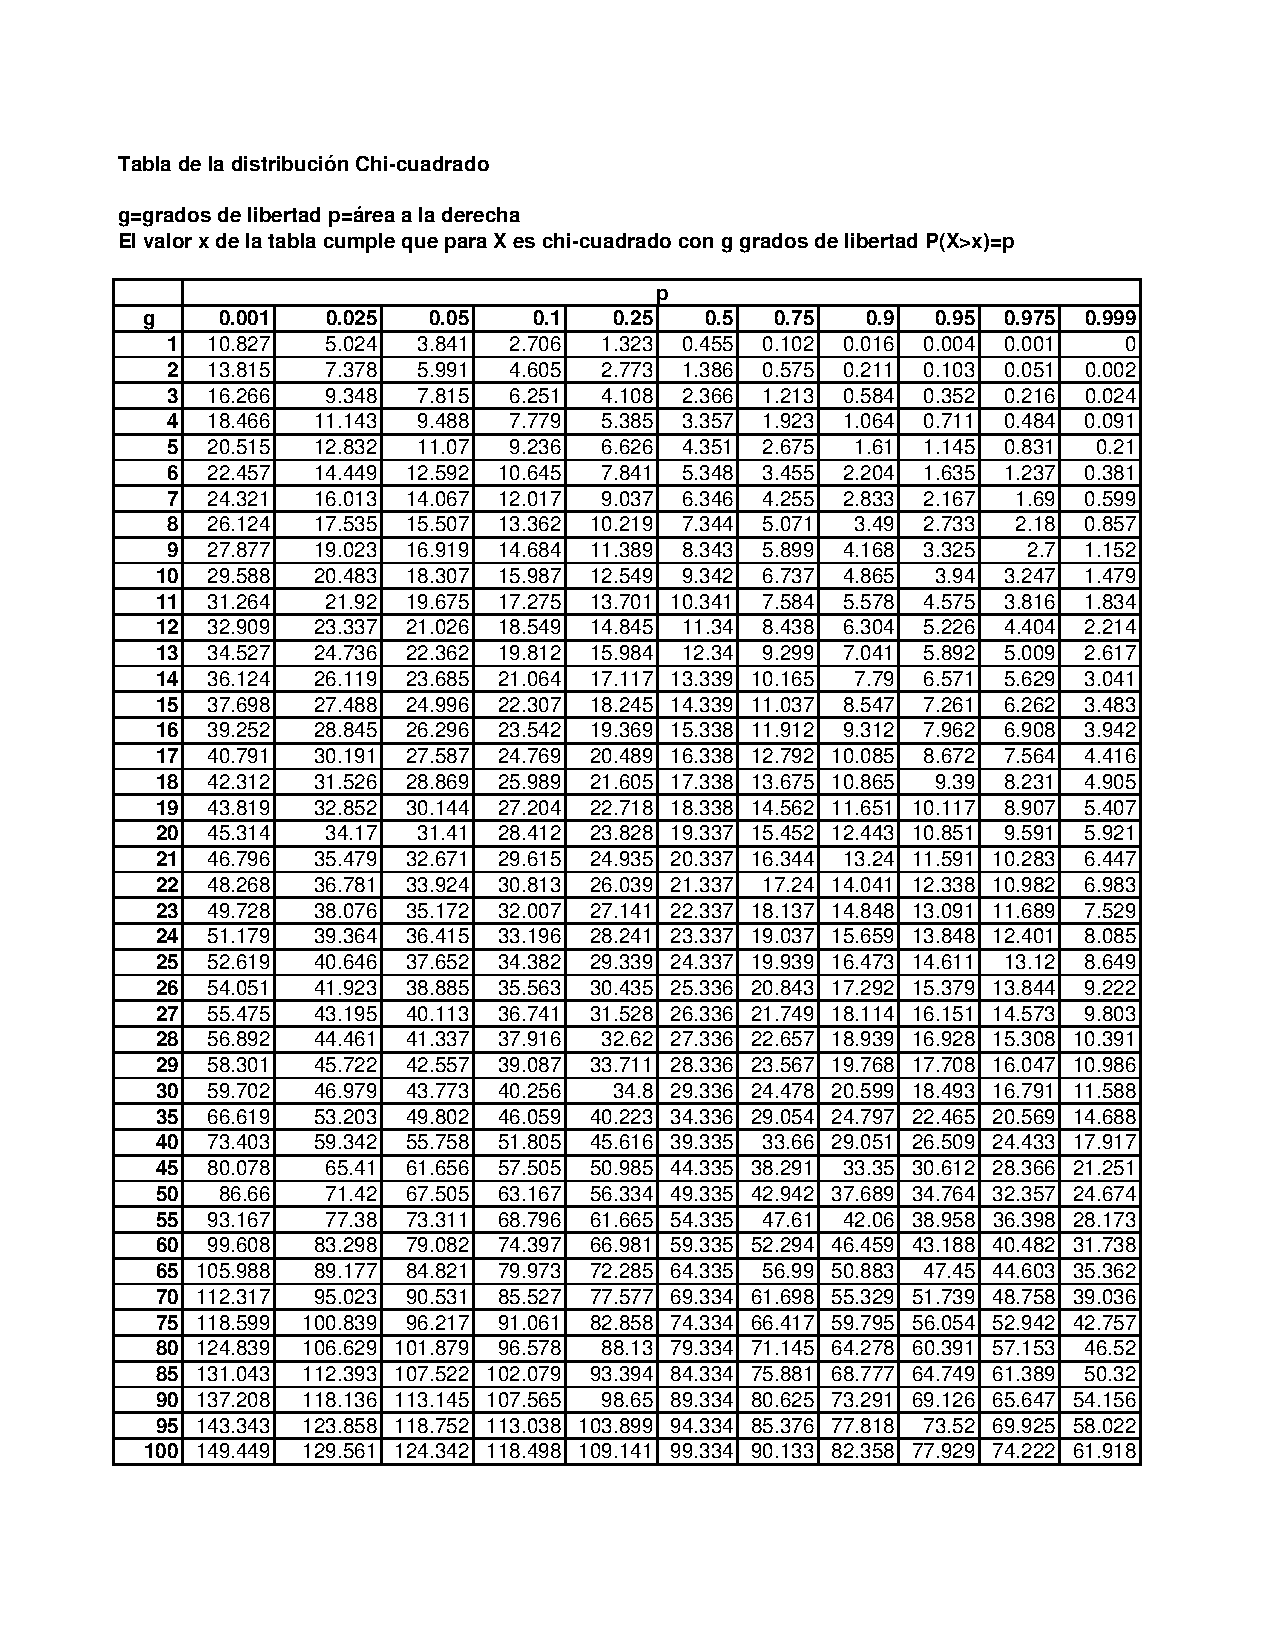
\includepdf[pages={1}]{pdf/_chicuadrado.pdf}


\chapter{Prácticas}
Se incluyen las soluciones de las prácticas:
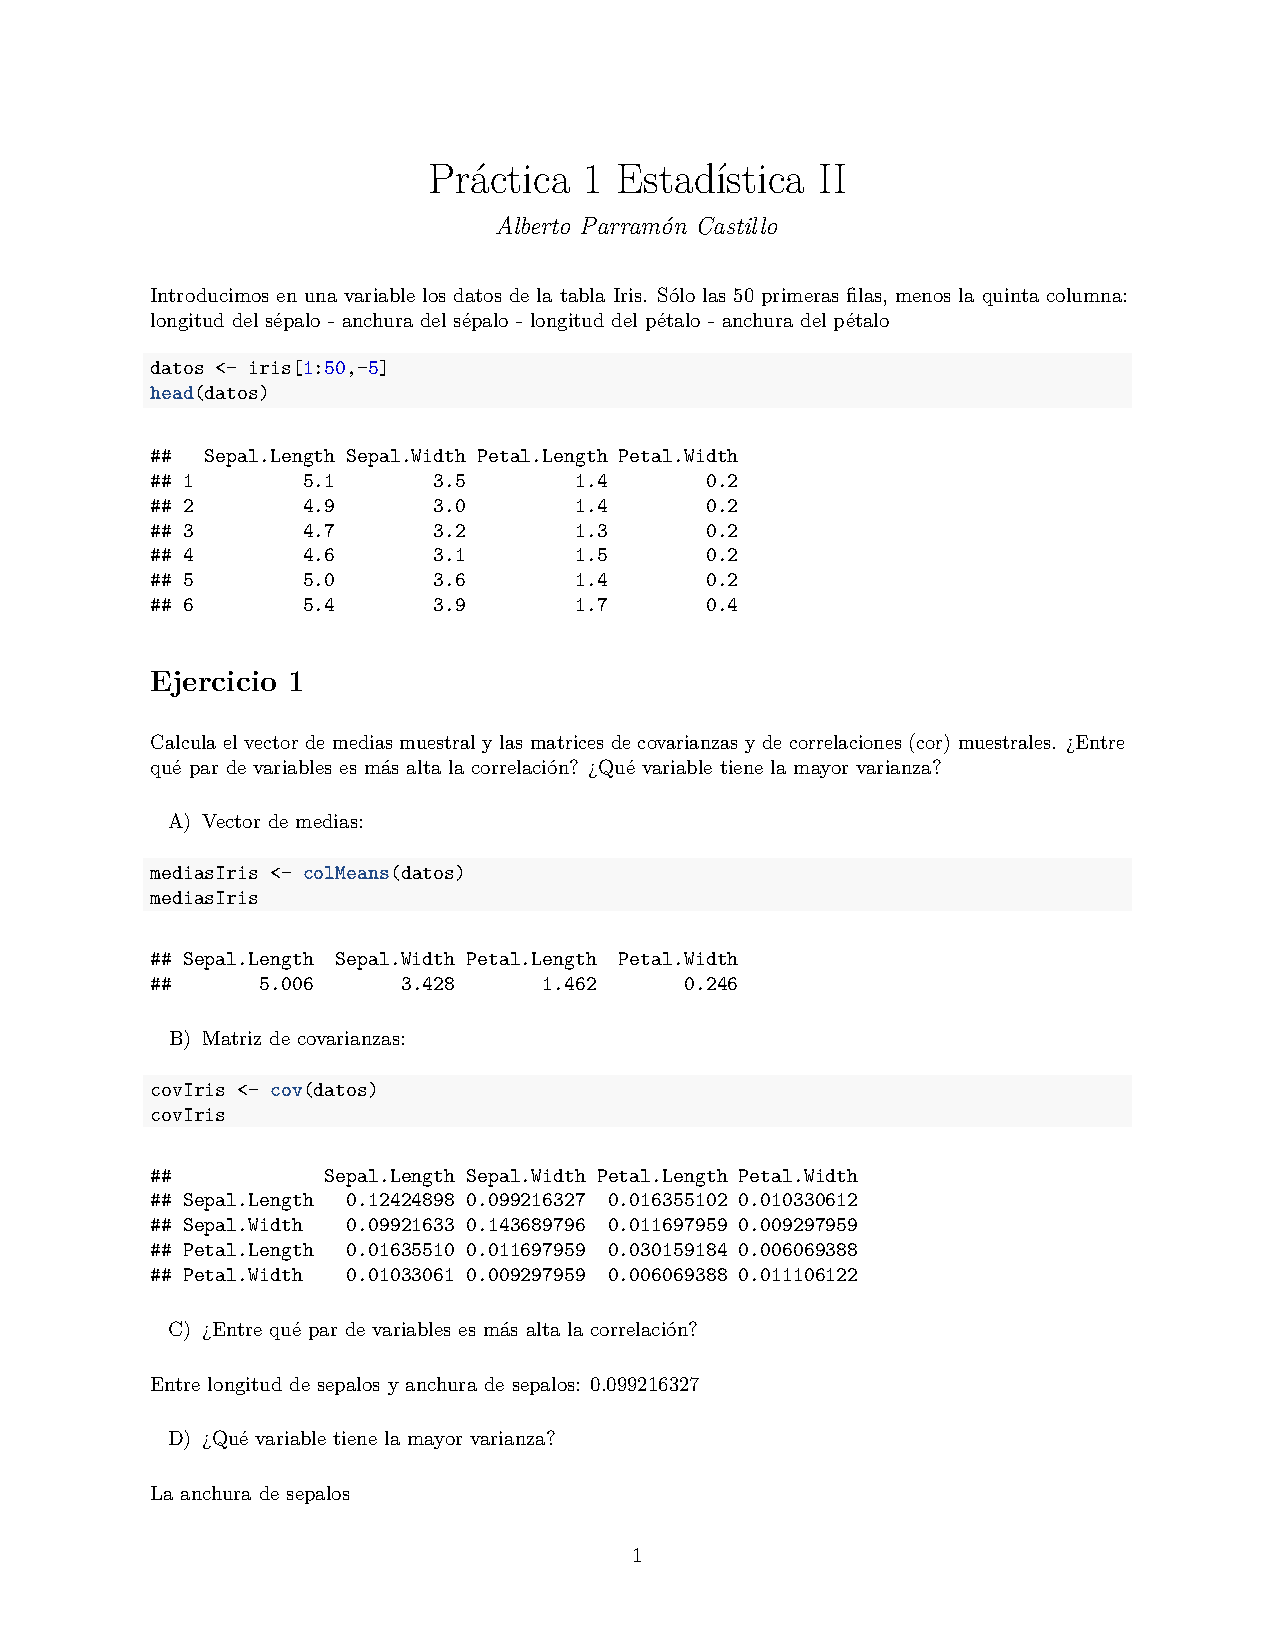
\includepdf[pages={1-6}]{pdf/_p1E2.pdf}
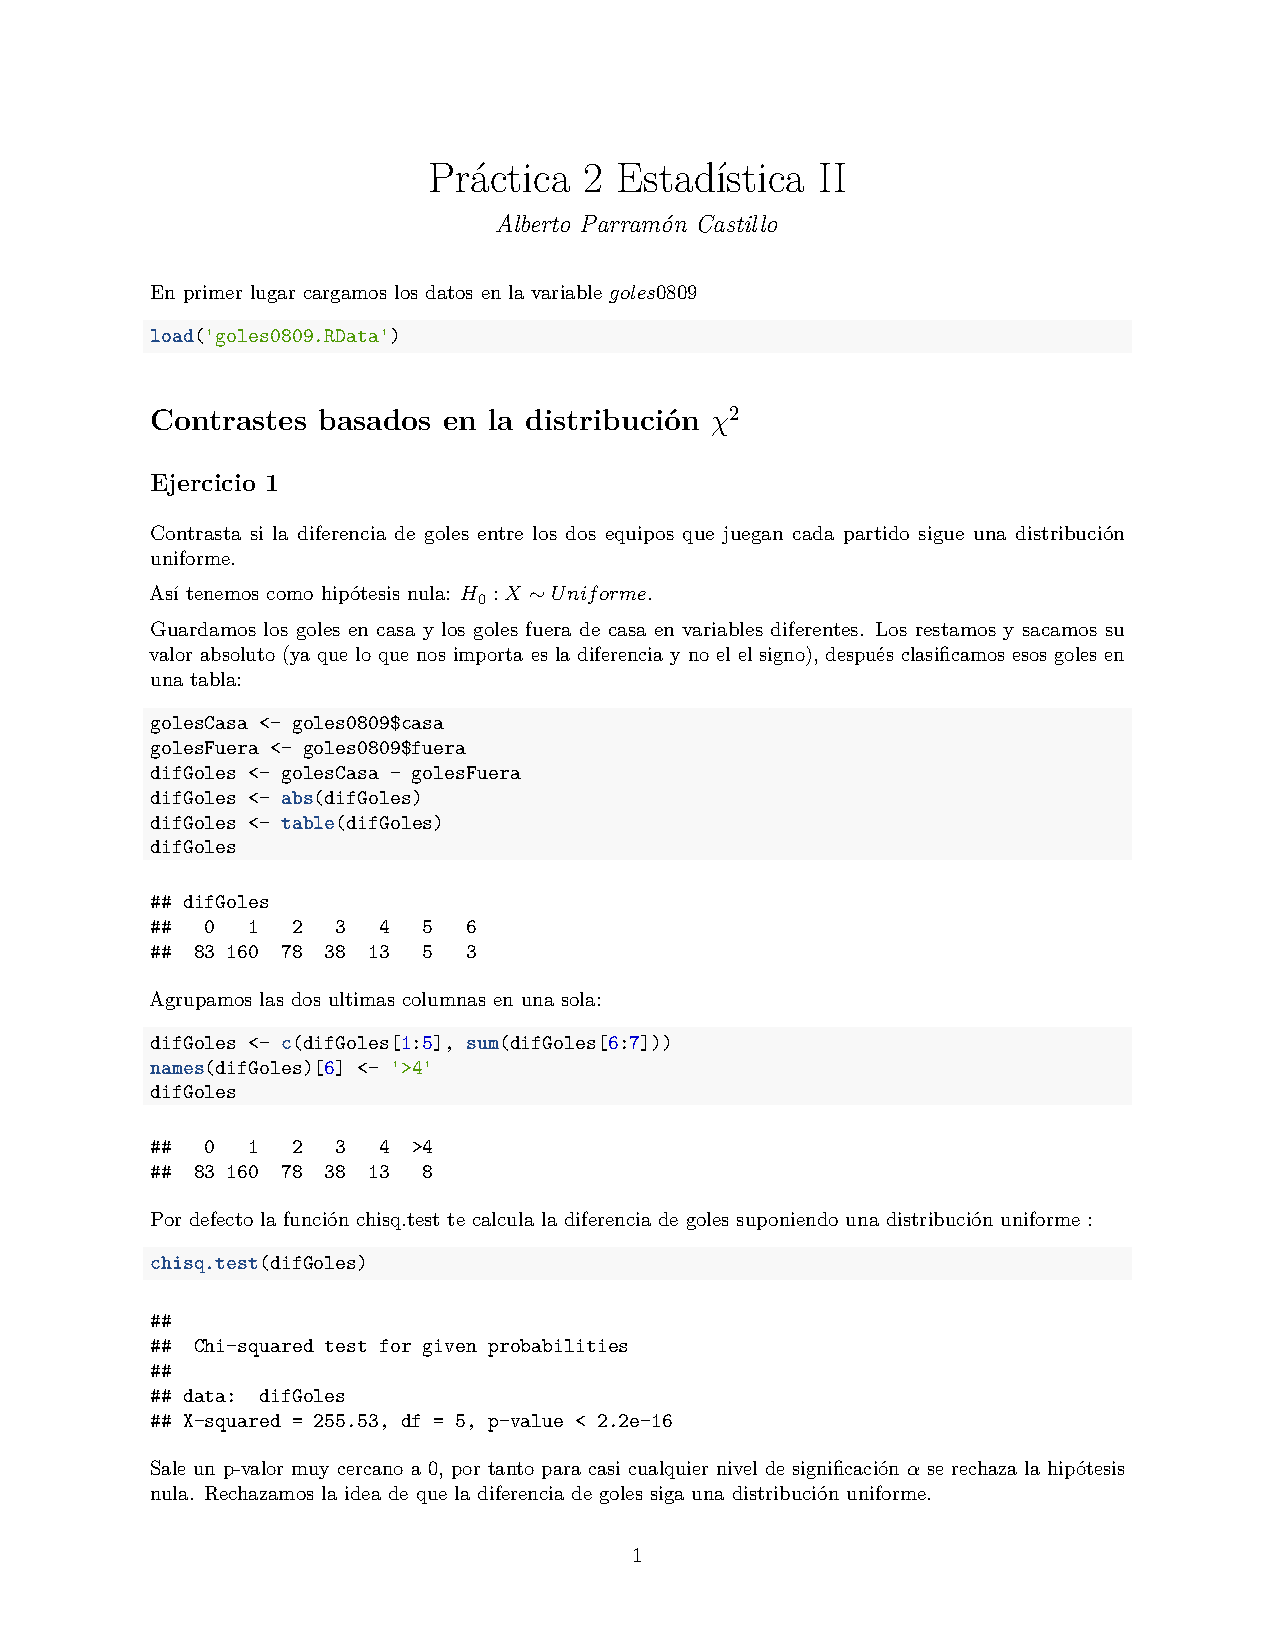
\includepdf[pages={1-8}]{pdf/_p2E2.pdf}

\bibliography{../Apuntes}{}

\printindex

\end{document}

